\documentclass{ctexart}
\usepackage{xeCJK}
\usepackage{fontspec}
% 设置全局字体为楷体
\setCJKmainfont{KaiTi}[
    BoldFont={SimHei}, % 使用黑体作为粗体
    ItalicFont={STXinwei}, % 使用楷体作为斜体
    BoldItalicFont={SimHei} % 使用黑体作为粗斜体
]
% 设置英文字体
\setmainfont{Times New Roman}

% 设置页面
\usepackage{geometry}
\usepackage{tabularx}
\usepackage{array}
\usepackage{float}
\usepackage{wrapfig}
\usepackage{lastpage}
\usepackage{titlesec}
\usepackage{indentfirst}
\usepackage{tikz}
\usepackage{everypage}
\usepackage{caption}
\captionsetup[figure]{labelformat=empty}
\usepackage{xcolor}
\usepackage{listings}
\usepackage{hyperref} % 超链接
\usepackage{tikz}
% 插图片
\usepackage{graphicx}
% 设置摘要页缩减 
\usepackage{changepage}
% 设置页眉页脚
\usepackage{fancyhdr}
\setlength{\headheight}{12.64723pt}
\addtolength{\topmargin}{-0.64723pt}
% 清空页眉页脚
\pagestyle{fancy}
% 设置列表缩进
\usepackage[shortlabels]{enumitem}
% 设置修改默认的section标题大小
\usepackage{titlesec}
\titleformat*{\section}{\LARGE}
\titleformat*{\subsection}{\Large}
\titleformat*{\subsubsection}{\Large}
% 使用数学宏包
\usepackage{amsmath}
% 设置表格的列格式
\usepackage{array}
% 三线表宏包
\usepackage{booktabs}
% 设置产考文献不输出默认名
\usepackage{etoolbox}
\patchcmd{\thebibliography}{\section*{\refname}}{}{}{}
% 引入网站作为参考文献
\usepackage{url}
% 设置等宽的代码字体
\setmonofont{Courier New}
% 颜色
\usepackage{xcolor}
% 代码高亮方案宏包
\usepackage{listings}
\definecolor{CPPLight}  {HTML} {686868}
\definecolor{CPPSteel}  {HTML} {888888}
\definecolor{CPPDark}   {HTML} {262626}
\definecolor{CPPBlue}   {HTML} {4172A3}
\definecolor{CPPGreen}  {HTML} {487818}
\definecolor{CPPBrown}  {HTML} {A07040}
\definecolor{CPPRed}    {HTML} {AD4D3A}
\definecolor{CPPViolet} {HTML} {7040A0}
\definecolor{CPPGray}  {HTML} {B8B8B8}
\lstset{
	basicstyle=\ttfamily,
	breaklines=true,
	framextopmargin=50pt,
	frame=bottomline,
	columns=fixed,       
    %numbers=left,                                       % 在左侧显示行号
	frame=none,                                          % 不显示背景边框
	backgroundcolor=\color[RGB]{255,255,255},            % 设定背景颜色
	keywordstyle=\color[RGB]{40,40,255},                 % 设定关键字颜色
	numberstyle=\footnotesize\color{darkgray},           % 设定行号格式
	commentstyle=\itshape\color[RGB]{0,96,96},                % 设置代码注释的格式
	stringstyle=\slshape\color[RGB]{128,0,0},   % 设置字符串格式
	showstringspaces=false,                              % 不显示字符串中的空格
	language=python,                                     % 设置语言
	morekeywords={alignas,continute,friend,register,true,alignof,decltype,goto,
		reinterpret_cast,try,asm,defult,if,return,typedef,auto,delete,inline,short,
		typeid,bool,do,int,signed,typename,break,double,long,sizeof,union,case,
		dynamic_cast,mutable,static,unsigned,catch,else,namespace,static_assert,using,
		char,enum,new,static_cast,virtual,char16_t,char32_t,explict,noexcept,struct,
		void,export,nullptr,switch,volatile,class,extern,operator,template,wchar_t,
		const,false,private,this,while,constexpr,float,protected,thread_local,
		const_cast,for,public,throw,std},
	emph={map,set,multimap,multiset,unordered_map,unordered_set,numpy,graph,path,append,extend,
		unordered_multiset,unordered_multimap,vector,string,list,deque,
		array,stack,forwared_list,iostream,memory,shared_ptr,unique_ptr,
		random,bitset,ostream,istream,cout,cin,endl,move,default_random_engine,
		uniform_int_distribution,iterator,algorithm,functional,bing,numeric,},
	emphstyle=\color{CPPViolet}, 
}

% 绘制页面边框
\usepackage{everypage}
\AddEverypageHook{
  \begin{tikzpicture}[remember picture, overlay]
    \draw[thick] ([xshift=0.5cm, yshift=0.5cm]current page.south west) rectangle ([xshift=-0.5cm, yshift=-0.5cm]current page.north east);
  \end{tikzpicture}
}

% 设置自定义字体
\newfontfamily\customfont{Freestyle Script}
\newfontfamily\haettenfont{Haettenschweiler}
\setCJKfamilyfont{xw}{STXinwei}
\newcommand{\xw}[1]{{\CJKfamily{xw}#1}}


\begin{document}

% 标题页
\begin{titlepage}
    \centering
    \vspace*{96pt}
    
\includegraphics[width=1\textwidth]{pics/cup.png}\par
    \fontsize{26}{31.2}\selectfont{中国石油大学(北京)吃饭指北}\par % 主标题
    \fontsize{18}{21.6}\selectfont{China University of Petroleum Dining Guide \customfont (CUPDG)}\par % 英文标题
    \vspace{39pt}
    \fontsize{22}{26.4}\selectfont{\haettenfont v5. 0. 1\normalfont }\par % 版本
    \vspace{52.8pt}
    \fontsize{18}{21.6}\selectfont{作者:刈夫和石大的同学们}\par % 作者
    \fontsize{18}{21.6}\selectfont{最后编辑时间:2024年9月17日}\par % 最后编辑时间
    \vfill
\end{titlepage}

% 目录页
\newpage
\thispagestyle{empty}
\footnotesize
\tableofcontents
\newpage
% 目录页后面是第一页
\setcounter{page}{1}

% 开始写正文
% 设置正文的页边距
\newgeometry{top=3cm, left=3.5cm, right=3.5cm}
% 设置正文的页眉页脚
\fancyhf{}
\fancyhead[C]{ }
% 此处修改右上角页码
\fancyhead[R]{Page \thepage\ of\ \NoHyper\pageref{LastPage}\endNoHyper}
\fancyhead[L]{\customfont CUPDG}
\fancyfoot[C]{\bfseries\thepage}
% 设置序言标题居中且不显示章节编号
\titleformat{\section}[block]{\normalfont\Large\bfseries\centering}{}{0pt}{}
\fontsize{26pt}{31.2pt}\selectfont
\vspace*{-50pt}
\textbf{\section{序言}}
\fontsize{14pt}{16.8pt}\selectfont
\noindent\makebox[\linewidth][c]{\textbf{第5版}}
\addcontentsline{toc}{subsection}{1.1 \ 第5版}
\setlength{\parindent}{2em} % 设置首行缩进为2字符

经过一段时间的积累,作者终于决定发布本指北的稳定版。(注:第5版和第4版的最大区别就是\textbf{目录增加了超链接},现在可以直接从目录点到对应的内容去)

作者在以往版本中对指北内容进行了多次修改,经过时间的积淀,在目前版本中,已经完成了对校内校外大部分优质店铺的介绍,希望同学们能多多宣传,帮助更多的同学。

但是我们的脚步不会就此停止,作者仍然接受任何同学分享的信息,也会亲自尝试更多店铺。希望各位同学继续保持探索的热情,在这片美食荒漠中挖掘井泉,滋润一年又一年的同学。毕竟:

\textbf{窗边何必冰凉雨,自是美食忆永年。}
\vspace{16.8pt}
\begin{flushright}
	\xw{刈夫}
	
	2024年9月10日
\end{flushright}

\vspace*{33.6pt}
喜讯,本项目已经\textbf{上传Github},欢迎大家前往查看!

\href{https://github.com/Octopus058/China-University-of-Petroleum-Dining-Guide}{Github Repository (CUPDG)}

麻烦大家\textbf{点个小小的star},如果有任何意见,请\textbf{直接发起PR},作者会不定期查看处理。
\begin{flushright}
	\xw{刈夫}
	
	2024年9月17日
\end{flushright}
\newpage

\noindent\makebox[\linewidth][c]{\textbf{第2版}}
\addcontentsline{toc}{subsection}{1.2 \ 第2版}
\setlength{\parindent}{2em} % 设置首行缩进为2字符

作者对单调的学校食堂感到厌倦,加上下课时间调整后根本抢不上食堂座位被迫去外面吃。于是痛定思痛,常常在学校周围发掘宝藏小店,经过道听途说与不断尝试,有了一定积累。本来这些信息只在同班同学和老乡间传播,2024年8月31日下午,作者突发奇想,想把所有店总结一下,因此决定撰写本指北。

本攻略暂时将分为两部分,第一部分是校内窗口,第二部分是校外店铺,未来可能加入其他内容,尚未下定论。需要特别注意的是,本指北将不包含外卖内容(因为作者从不点外卖),我想,只有在正确的地方才能吃出正确的味道,让我们走出宿舍,多跑两步,体验一下学习之余美好的大学生活吧。

另外,欢迎大家向作者分享更多宝藏店铺,让这份指北更加充实。作者QQ:2379401911,VX:Octopus058,不胜感激!
\vspace{16.8pt}
\begin{flushright}
	\xw{刈夫}
	
	2024年8月31日
\end{flushright}

\newpage
\titleformat{\section}[block]{\normalfont\Large\bfseries\centering}{}{0pt}{}
\fontsize{26pt}{31.2pt}\selectfont
\vspace*{-50pt}
\textbf{\section{校内}}
\vspace*{-20pt}
\textbf{\subsection*{一、基本伙}}
\addcontentsline{toc}{subsection}{2.1 \ 基本伙}
\fontsize{14pt}{16.8pt}\selectfont
\setlength{\parindent}{2em} % 设置首行缩进为2字符
既然叫基本伙了,自然不要求他色香味俱全,你油的一餐一楼,二餐一楼,三餐一楼,一餐三楼的一部分都是基本伙,价格一般情况下在0-11元不等,一碗菜2-4元,一碗肉4-6元,有些特殊菜可能6-10元,米饭大中小分别八毛五毛三毛,如果按两菜一肉的话8-10块差不多了。

另外,不同食堂的口味也不太一样,一餐三餐重口味,二餐经常过于清淡。不过这件事就见仁见智了,仅供各位参考。

\textbf{\subsection*{二、风味窗口}}
\addcontentsline{toc}{subsection}{2.2 \ 风味窗口}
\fontsize{14pt}{16.8pt}\selectfont
\setlength{\parindent}{2em} % 设置首行缩进为2字符
润杰的风味档口,小面和米线还行,其他没吃过,蹲一个吃过的同学提供意见。感觉价格有点小贵,主要是图个方便,比外卖更快。

一餐二三四楼的风味窗口,经过种种变迁,消失了很多,留下的之中自然有精品,作者总结下来是这样的:

二楼17块钱炒鸡,尤其是柠檬炒鸡和香辣炒鸡,整个一餐唯一能让人吃四碗饭的窗口(就是为了这个汤要的这碗饭),不必多说。

二楼米高林铁板烧,每次看到这个名字都会想它和米其林什么关系。个人感觉意面不好吃,米饭的还可以。量可能略微有点少,食量大的同学可以考虑回宿舍吃个面包。

二楼夹馍,菜的4块肉的8块,想吃点清淡的时候可以考虑。

三楼和四楼麻辣香锅,放在一起讲。三楼通常更咸,四楼偶尔可能不太卫生。\textbf{(提供者:GF)}昌平最便宜的麻辣香锅没有之一。不能吃辣的同学建议微辣,能吃辣的同学建议特辣(也不是特别辣)。作者的吃法是方便面加一碗米饭,直接放一起吃,同学们可以参考一下。

\begin{figure}[ht]
	\centering
	\includegraphics[width=0.63\textwidth]{pics/校内/炒鸡.jpg}
	\caption{香辣炒鸡yyds} 
\end{figure}
四楼烤鱼,多人食堂聚餐首选,作者的建议是3人吃2条鱼比较合适,2人1条可能有点少,另外就是除了烤鱼也可以烤鸡腿之类的,体验都还不错。

\begin{figure}[ht]
	\centering
	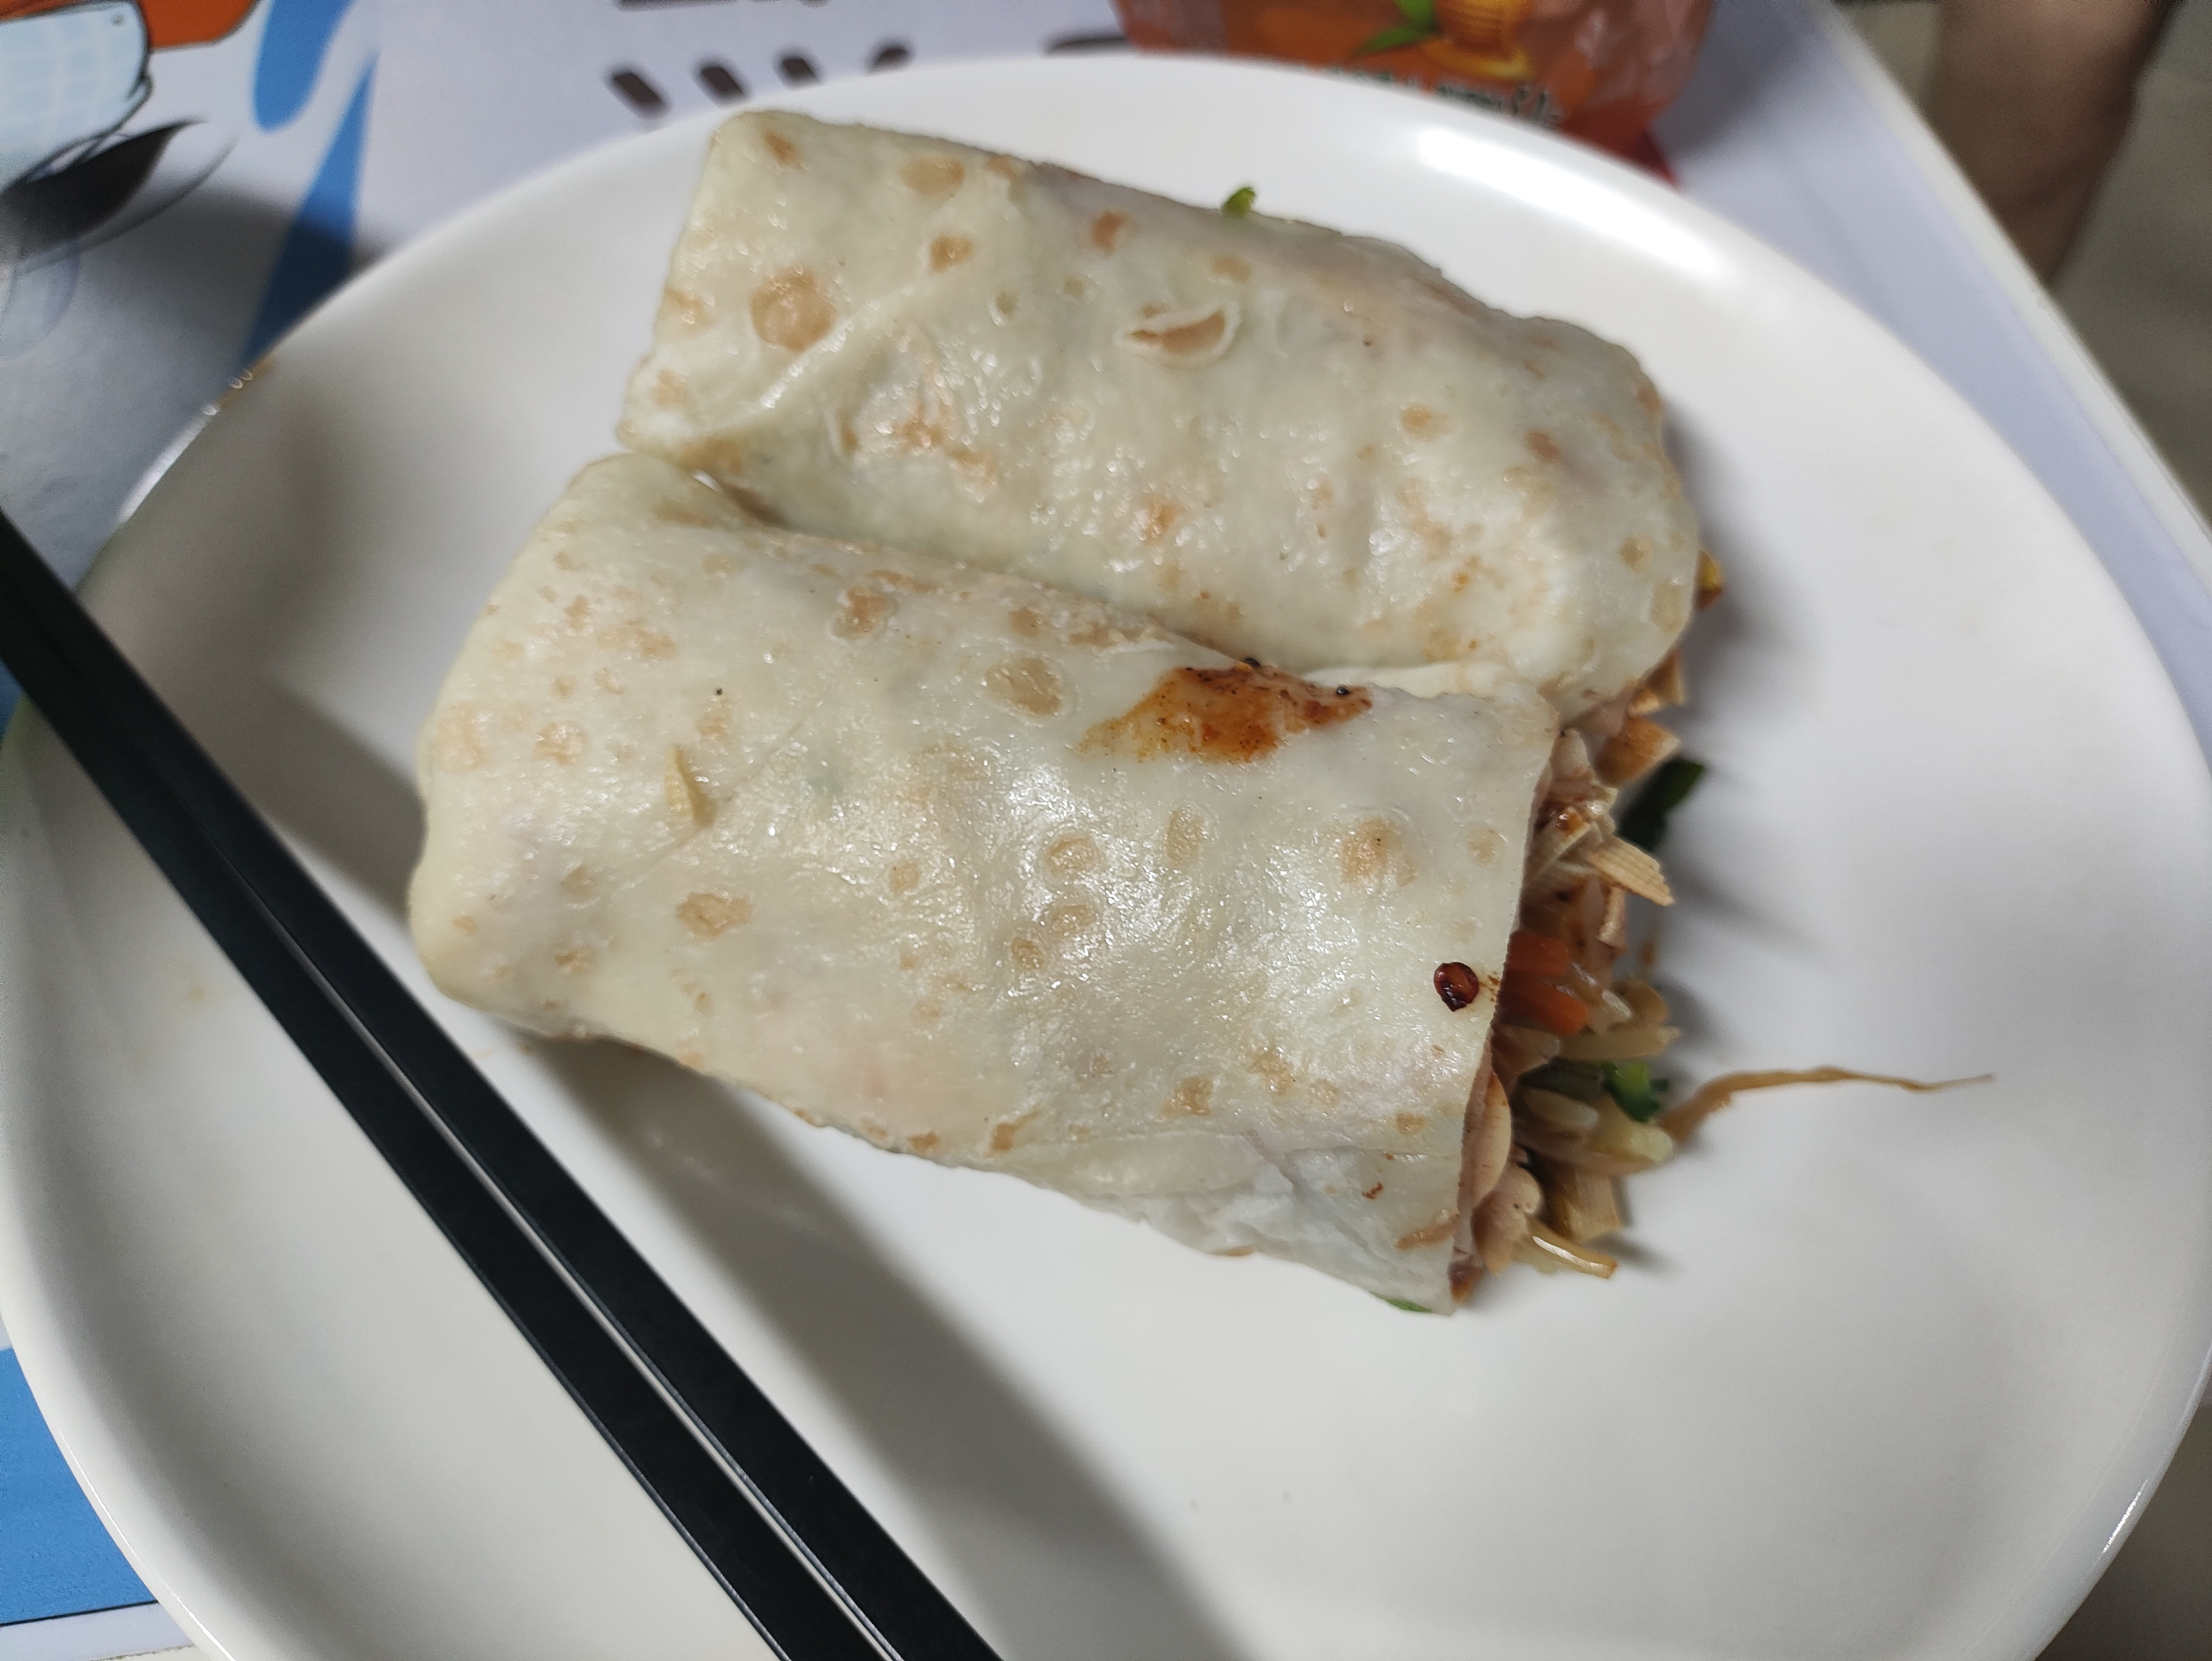
\includegraphics[width=0.63\textwidth]{pics/校内/卷饼.jpg}
	\caption{这是一个,不是两个} 
\end{figure}
四楼9/7块卷饼,体验和二楼夹馍差不多,但是够大,性价比挺高,有时候吃一个就饱了。

四楼米线,作为禾苑后时代的遗留产物,价格有点高,米线就和当年的面一样煮的大劲,一模一样的风格,看个人习惯。但无论如何,禾苑永远活在我们心中。
\begin{figure}[ht]
	\centering
	\includegraphics[width=0.63\textwidth]{pics/校内/米线.jpg}
	\caption{欢迎旧王}
\end{figure}

\textbf{\subsection*{三、智选}}
\addcontentsline{toc}{subsection}{2.3 \ 智选}
\fontsize{14pt}{16.8pt}\selectfont
\setlength{\parindent}{2em} % 设置首行缩进为2字符
二餐二楼和三餐二楼,你问好吃吗?当然好吃,你问价格怎么样,只能说贵的实在离谱,拿点肉就好几十,吓得作者再也不敢去了。富哥和放纵餐首选。

\textbf{\subsection*{四、禾苑}}
\addcontentsline{toc}{subsection}{2.4 \ 禾苑}
\fontsize{14pt}{16.8pt}\selectfont
\setlength{\parindent}{2em} % 设置首行缩进为2字符
禾苑在经过一次脱胎换骨后成功损失了它的灵魂也就是面,作者对此感到万分悲痛。但是生活还是要继续,经过实地调查,作者重新挖掘出了禾苑的意义。对于一个人吃饭来说,现在大致可分为两种吃法,一种是盖饭,一种是小炒加一碗米饭,但是不少同学会觉得盖饭量少,六七分饱总差点意思。作者研究的结果是,盖饭可以加菜,有加3块和加5块两种,3块完全足矣,5块就太多了,然后过会再要一小碗饭即可(注意是小碗)。这样就可以从六分饱变成正好。

另外,千万避雷黑椒牛柳的小炒(大概叫这个),青椒洋葱远多于牛肉并且总量也很少。

最后的最后,如果有找到禾苑小面的同学请及时联系作者。米线目前已经发现,在一餐四楼。

\textbf{\subsection*{五、KFC}}
\addcontentsline{toc}{subsection}{2.5 \ KFC}
\fontsize{14pt}{16.8pt}\selectfont
\setlength{\parindent}{2em} % 设置首行缩进为2字符
有一说一非必要不去。大部分人只有疯狂星期四才去KFC,但是校内经常比润杰路口的东西还少,而且也没优惠。对于校内同学来说本来天堂般的享受丧失殆尽,直接去润杰路口的即可。

\textbf{\subsection*{六、新疆餐厅(提供者:润杰梁朝伟 \ GF)}}
\addcontentsline{toc}{subsection}{2.6 \ 新疆餐厅}
\fontsize{14pt}{16.8pt}\selectfont
\setlength{\parindent}{2em} % 设置首行缩进为2字符
一个字,跑;两个字,快跑!(手抓饭可以偶尔吃一次)

\textbf{\subsection*{七、翠宫}}
\addcontentsline{toc}{subsection}{2.7 \ 翠宫}
\fontsize{14pt}{16.8pt}\selectfont
\setlength{\parindent}{2em} % 设置首行缩进为2字符
\begin{figure}[ht]
	\centering
	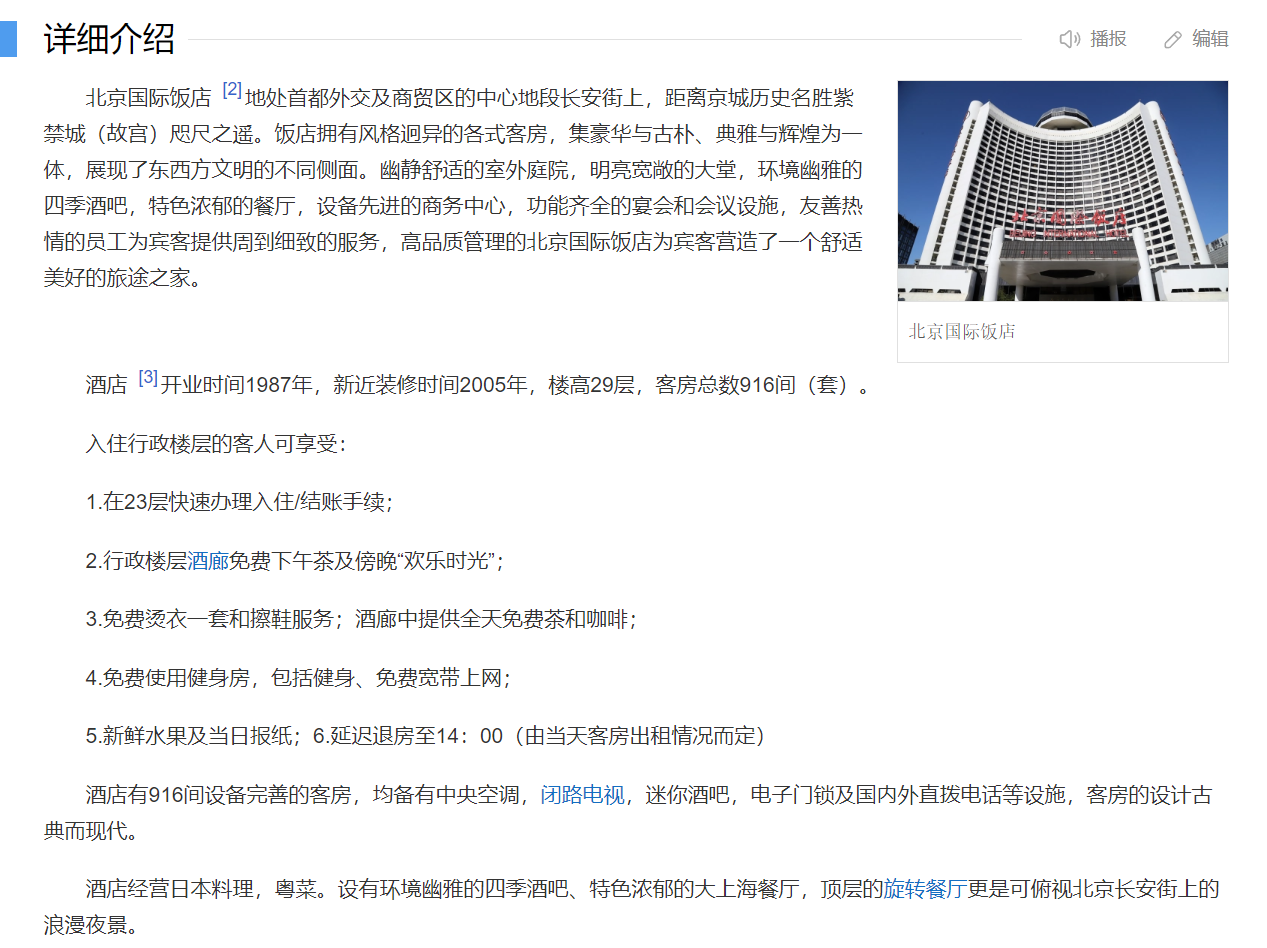
\includegraphics[width=0.73\textwidth]{pics/校内/国际饭店.jpg}
\end{figure}

\textbf{\subsection*{八、石大夜市(提供者:橘皮)}}
\addcontentsline{toc}{subsection}{2.8 \ 石大夜市}
\fontsize{14pt}{16.8pt}\selectfont
\setlength{\parindent}{2em} % 设置首行缩进为2字符
别问,问就是据说禾苑的小面去夜市了。我来夜市只办三件事,小面,小面,还是TMD小面!其他的?不熟!

\textbf{\subsection*{九、润杰食堂}}
\addcontentsline{toc}{subsection}{2.9 \ 润杰食堂}
\fontsize{14pt}{16.8pt}\selectfont
\setlength{\parindent}{2em} % 设置首行缩进为2字符
我吃的明明是炒饭,为什么却像坐在针毡上一样。我的手在抖,我的汗在流,舌头都咬出血了。此时此刻我真的破防了,破大防了,你滴的每一滴油都与我的心脏针锋相对。几乎都快羡慕得疯了,倒在床上蒙住被子就开始抱着枕头尖叫流泪,嘴里一边喊着救命救命,一边又忍着,我边发边哭,打字的手都是抖的,后来我的手抖得越来越厉害,从心头涌起的思想、情怀和梦想,这份歆羡和悔恨交织在一起,我的笑还挂在脸上,可是眼泪一下子就掉下来了。求你了别吃了,我生活再苦再难我都不会觉得难过,只有你们吃这盘炒饭的时候我的心里像被刀割一样的痛,打着字泪水就忍不住的往下流。我打开了手机,我看到你吃的炒饭,我感到了深深的差距,我卸载删除了一切社交软件,我拔了手机卡,我把自己蒙在被窝里一动不动,我耳边还是不停环绕你发的那些幸福生活,我直接跳进了家门口的井里。

\newpage
\titleformat{\section}[block]{\normalfont\Large\bfseries\centering}{}{0pt}{}
\fontsize{26pt}{31.2pt}\selectfont
\textbf{\section{校外}}
\textbf{\subsection*{一、南校园闸机口一条街}}
\addcontentsline{toc}{subsection}{3.1 \ 南校园闸机口一条街}
\fontsize{14pt}{16.8pt}\selectfont
\setlength{\parindent}{2em} % 设置首行缩进为2字符
这条街作为润杰的同学们上学的必经之路,人流量极大,而且离学校和宿舍都近,非常适合不想去食堂的同学们,我选了其中几个尤其好的店做详细的介绍。

\textbf{\subsubsection*{1. 高原拉面王}}
\addcontentsline{toc}{subsubsection}{3.1.1 \ 高原拉面王}
\begin{figure}[ht]
	\centering
	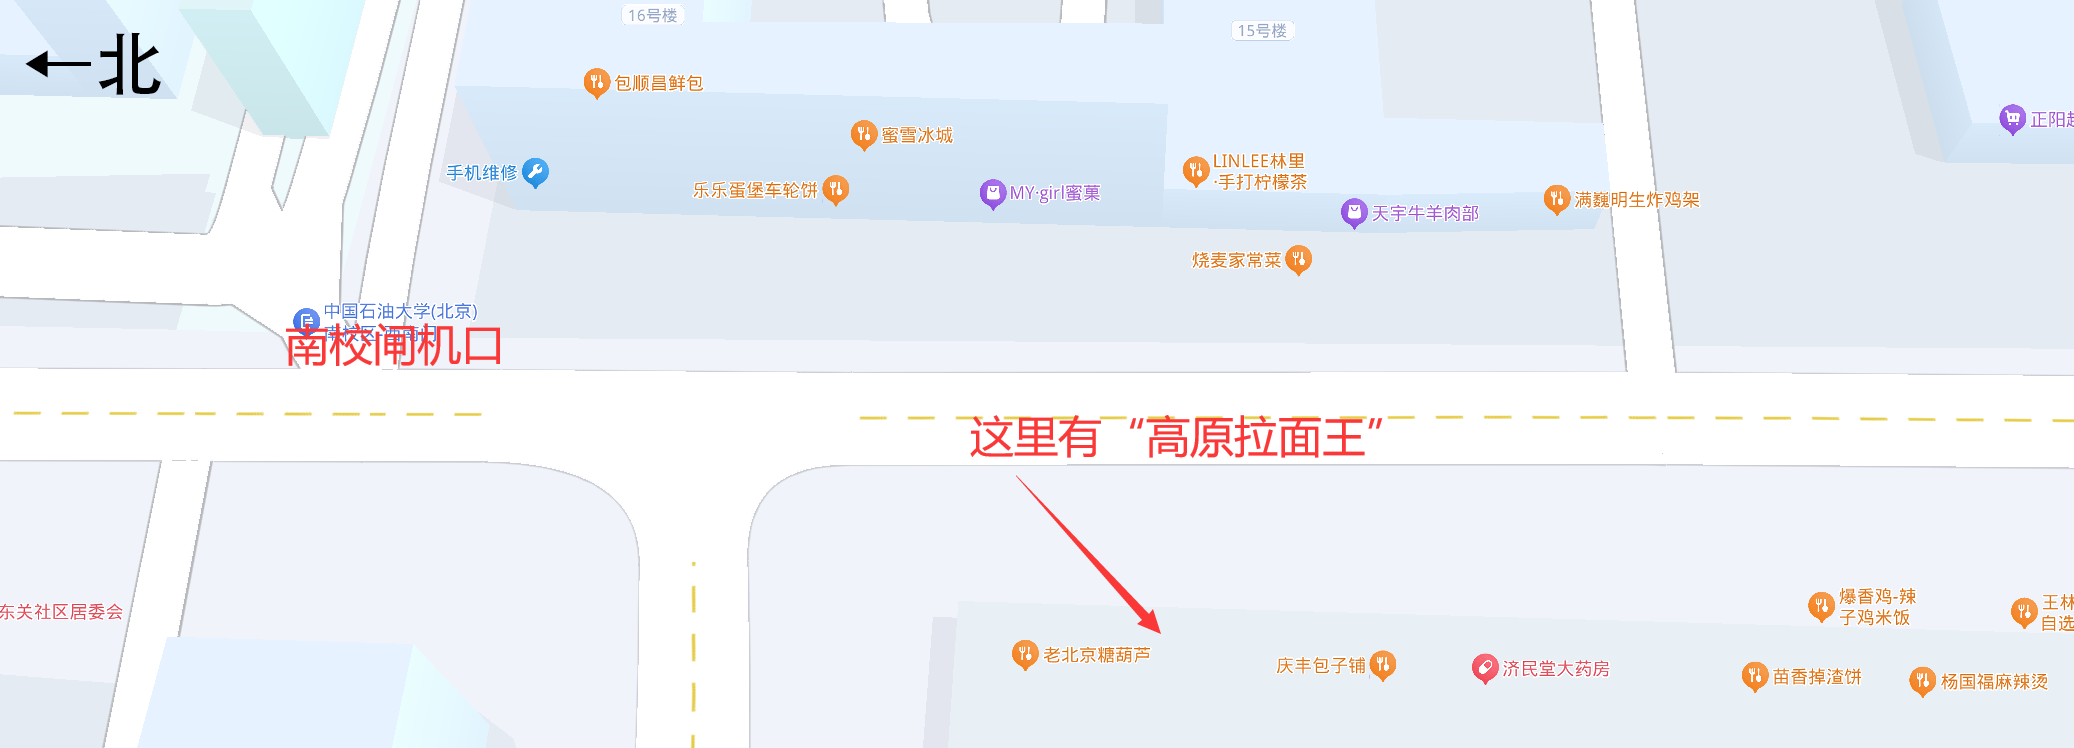
\includegraphics[width=0.9\textwidth]{pics/校外/南校/高原.png}
\end{figure}
把高原作为校外的第一个店,我觉得是非常合理的。高原的拉面拌面炒饭都很好,作者个人喜欢13块的拉面,13块的蛋炒饭,19块的大盘鸡拌面。我觉得应该让每个石大学生都吃过高原才对。

\textbf{\subsubsection*{2. 华莱士}}
\addcontentsline{toc}{subsubsection}{3.1.2 \ 华莱士}
\begin{figure}[ht]
	\centering
	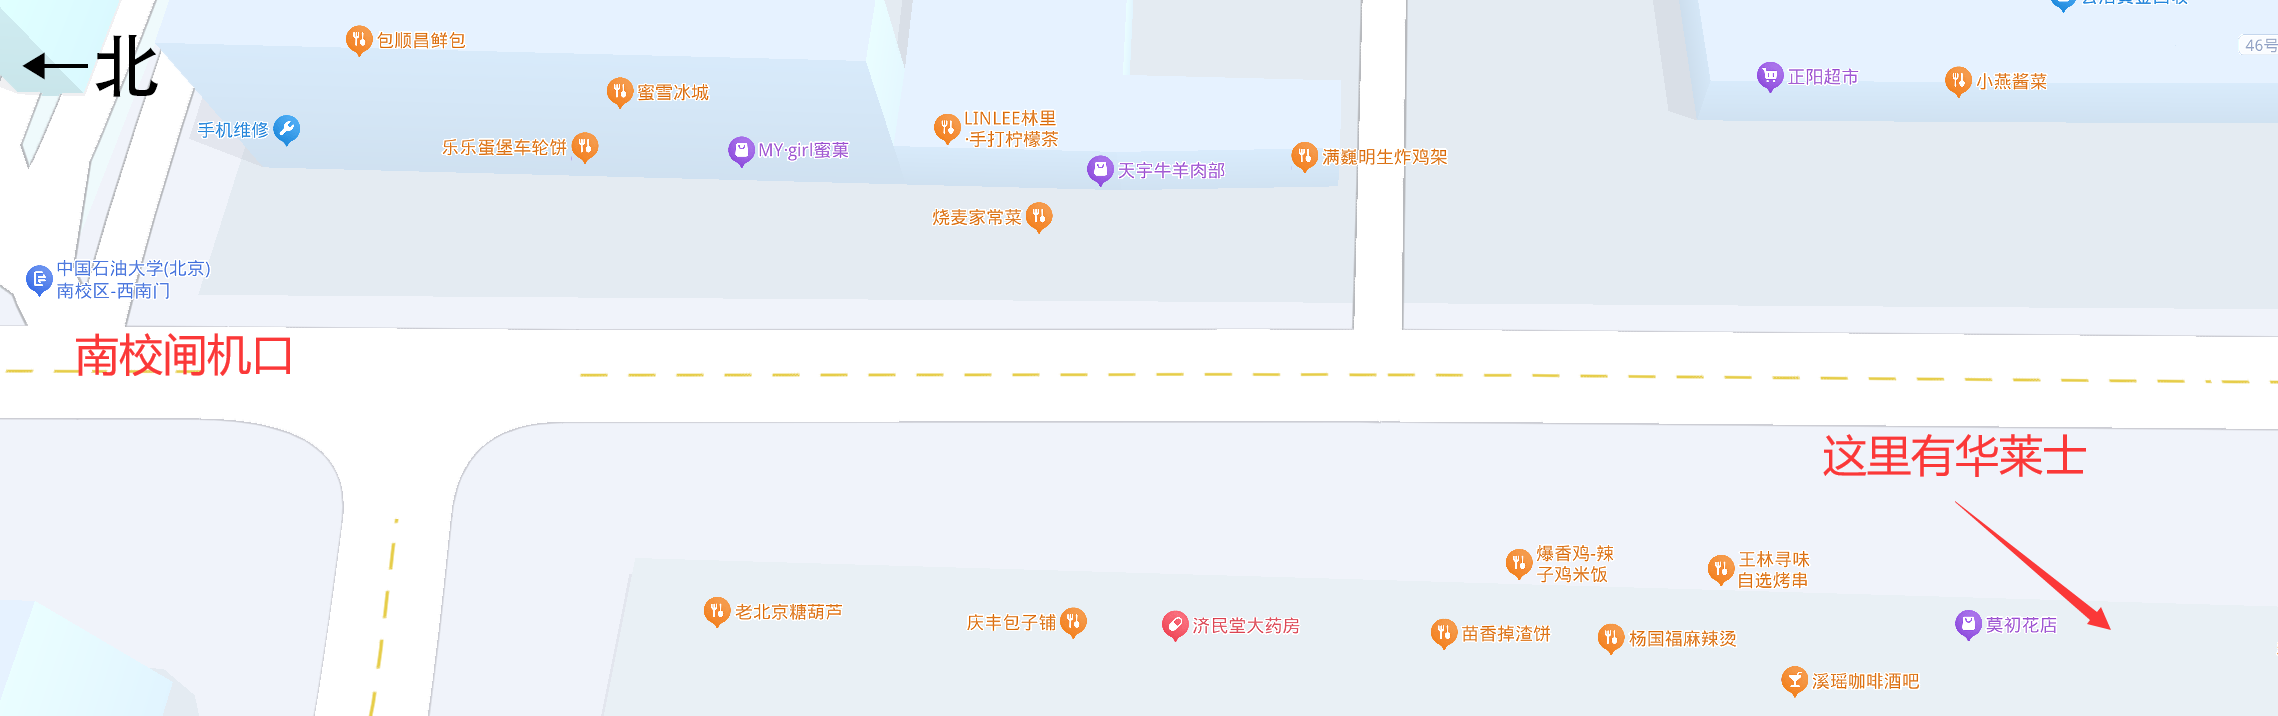
\includegraphics[width=0.85\textwidth]{pics/校外/南校/华莱士.png}
\end{figure}
华莱士常常被大家戏称“喷射战士”,但是我吃这家很多次了,没有出现过类似情况,可能是人流量大食材更新快的原因。因此,面对华莱士如此平民的价格,谁能不心动呢?

\textbf{\subsubsection*{3. 石锅鱼}}
\addcontentsline{toc}{subsubsection}{3.1.3 \ 石锅鱼}
\begin{figure}[ht]
	\centering
	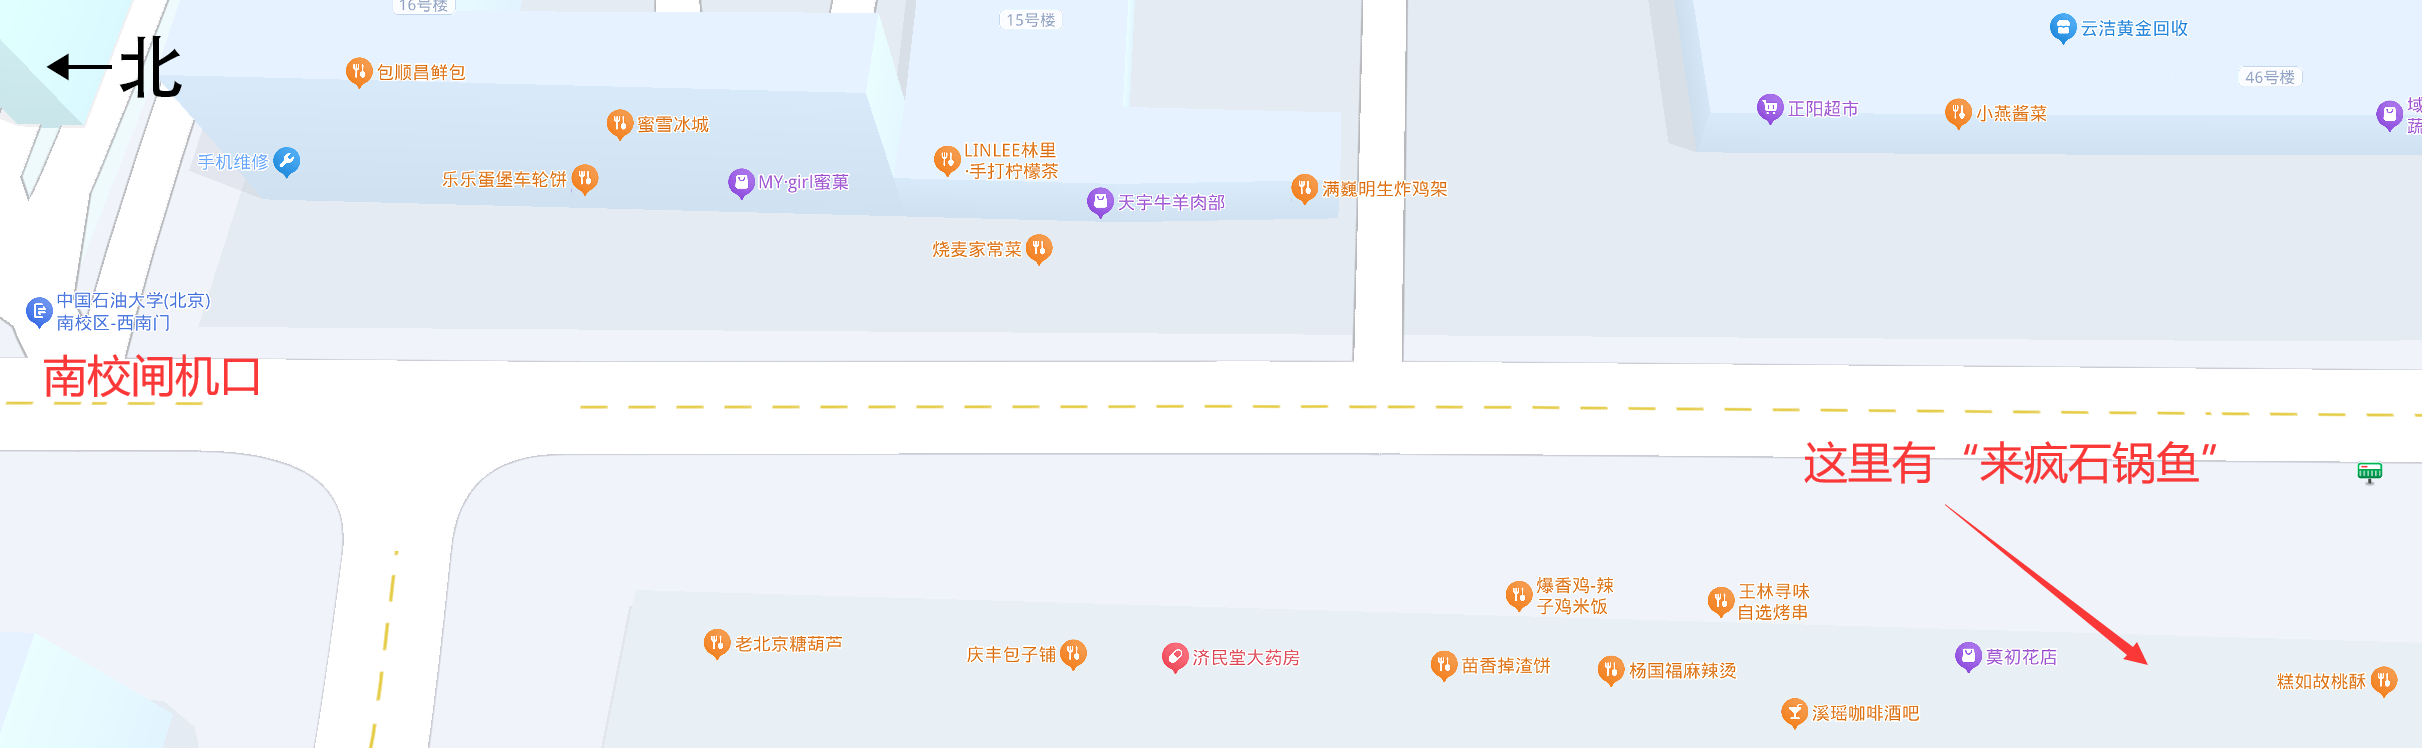
\includegraphics[width=0.85\textwidth]{pics/校外/南校/石锅鱼.png}
\end{figure}
这家店位置不错,但是知道的人不太多,就在华莱士旁边。美团上有双人套餐,55块钱左右,免费饮料米饭和小吃,体验非常不错,尤其是麻辣和青花椒口味。如果3人去,就点一个美团双人套餐和一个单人小锅,人均28-29左右。如果4人去,就点两个美团双人套餐。以此类推。

\textbf{\subsubsection*{4. 老曹家煎饼}}
\addcontentsline{toc}{subsubsection}{3.1.4 \ 老曹家煎饼}
\begin{figure}[ht]
	\centering
	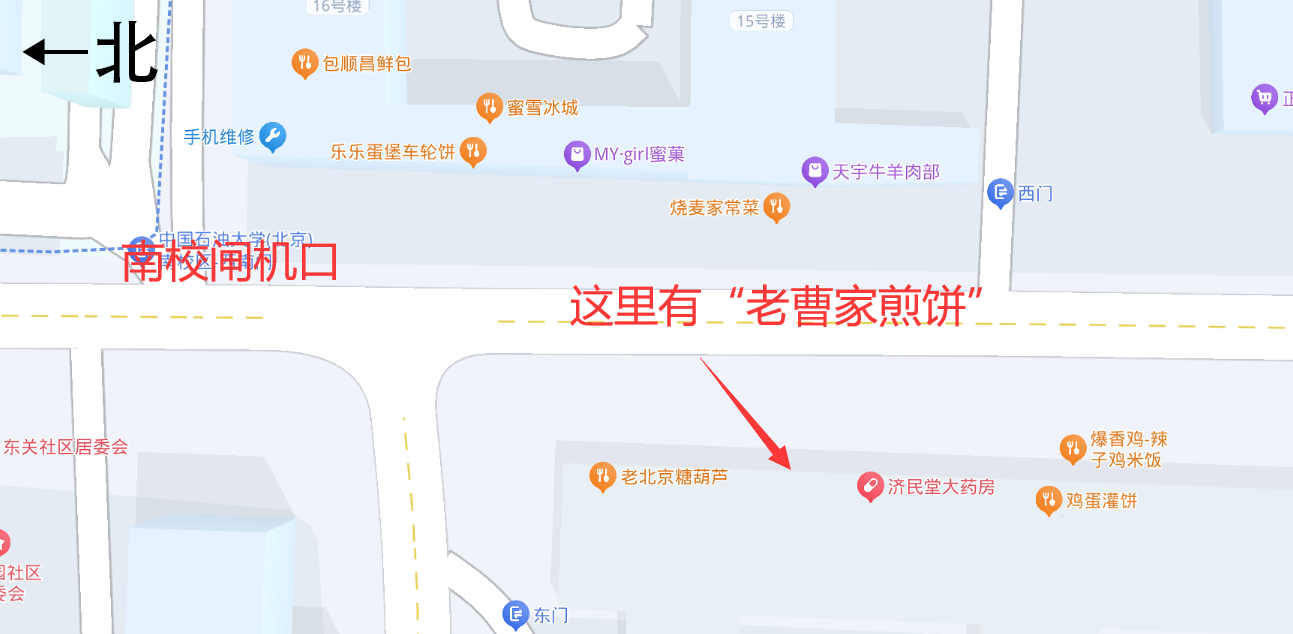
\includegraphics[width=0.7\textwidth]{pics/校外/南校/老曹家煎饼.png}
\end{figure}
这家煎饼应该是作者目前吃过的性价比最高的煎饼,量足实惠,如果你想可以试试他家38块钱的“牛B大煎饼”,还请告诉作者是什么感觉。

\textbf{\subsubsection*{5. 水萝卜}}
\addcontentsline{toc}{subsubsection}{3.1.5 \ 水萝卜}
不得不说,虽然有点小贵,仍然不影响水萝卜作为多人聚餐的圣地之一,即使不想吃饺子,也可以点普通菜,就像每次聚会的那样,普普通通才是真。
\begin{figure}[ht]
	\centering
	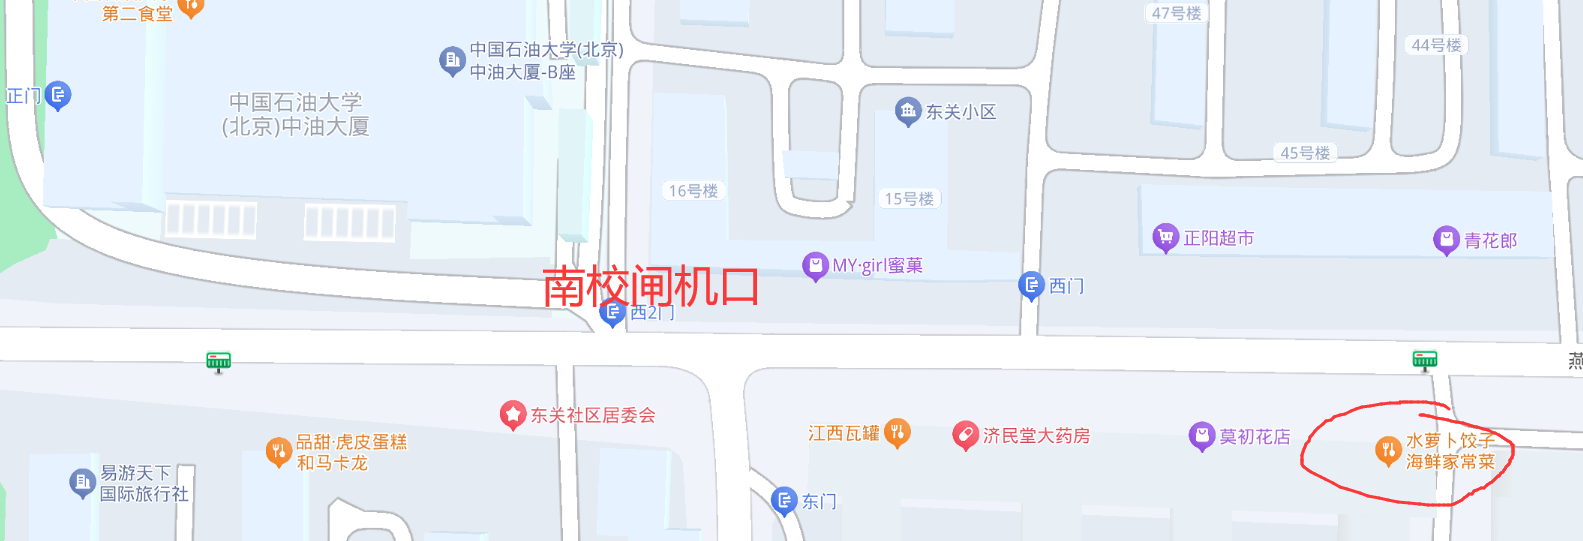
\includegraphics[width=0.9\textwidth]{pics/校外/南校/水萝卜.png}
\end{figure}

\newpage
\textbf{\subsection*{二、清秀园小区内}}
\addcontentsline{toc}{subsection}{3.2 \ 清秀园小区内}
\fontsize{14pt}{16.8pt}\selectfont
\setlength{\parindent}{2em} % 设置首行缩进为2字符
清秀园小区相对来说是一个偏僻的位置(知道的人不多),这里面藏着几个非常不错的店,完全值得吃四年那种。

\textbf{\subsubsection*{1. 川菜馆}}
\addcontentsline{toc}{subsubsection}{3.2.1 \ 川菜馆}
\begin{figure}[ht]
	\centering
	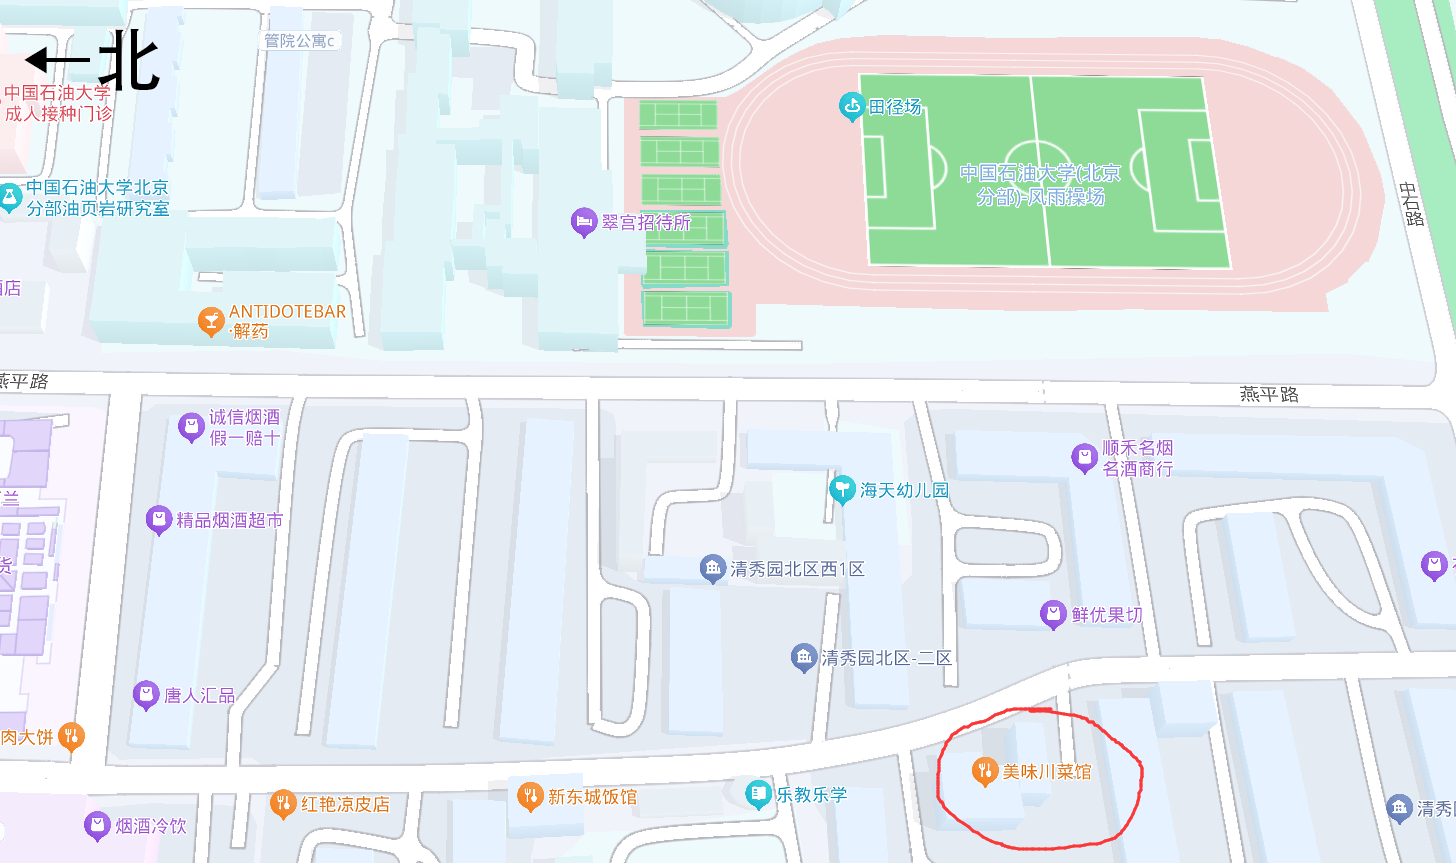
\includegraphics[width=0.8\textwidth]{pics/校外/清秀园/川菜馆.png}
\end{figure}
“求你让我再去一次川菜馆吧,我什么都会做的!”作者如是说道。在去川菜馆之前,要对自己的饭量有一个清楚的认识,不然很容易出现吃不完的情况。如果你是和同学去,我的建议是几个人就点几个菜。如果你是一个人去,建议点盖饭(量也很大)。建议做好剩菜的心理准备。另外,一定定定要点外婆菜炒鸡蛋,我觉得这道菜是完全可以看作镇店之宝的含金量。

\textbf{\subsubsection*{2. 烧饼店}}
\addcontentsline{toc}{subsubsection}{3.2.2 \ 烧饼店}
这家烧饼店老板娘一般看心情做啥种类的,价格比较便宜,很适合当懒得下馆子的时候随便吃两口的垫背。如果你运气好碰到有葱花烧饼的日子,无脑买就完事了。
\begin{figure}[ht]
	\centering
	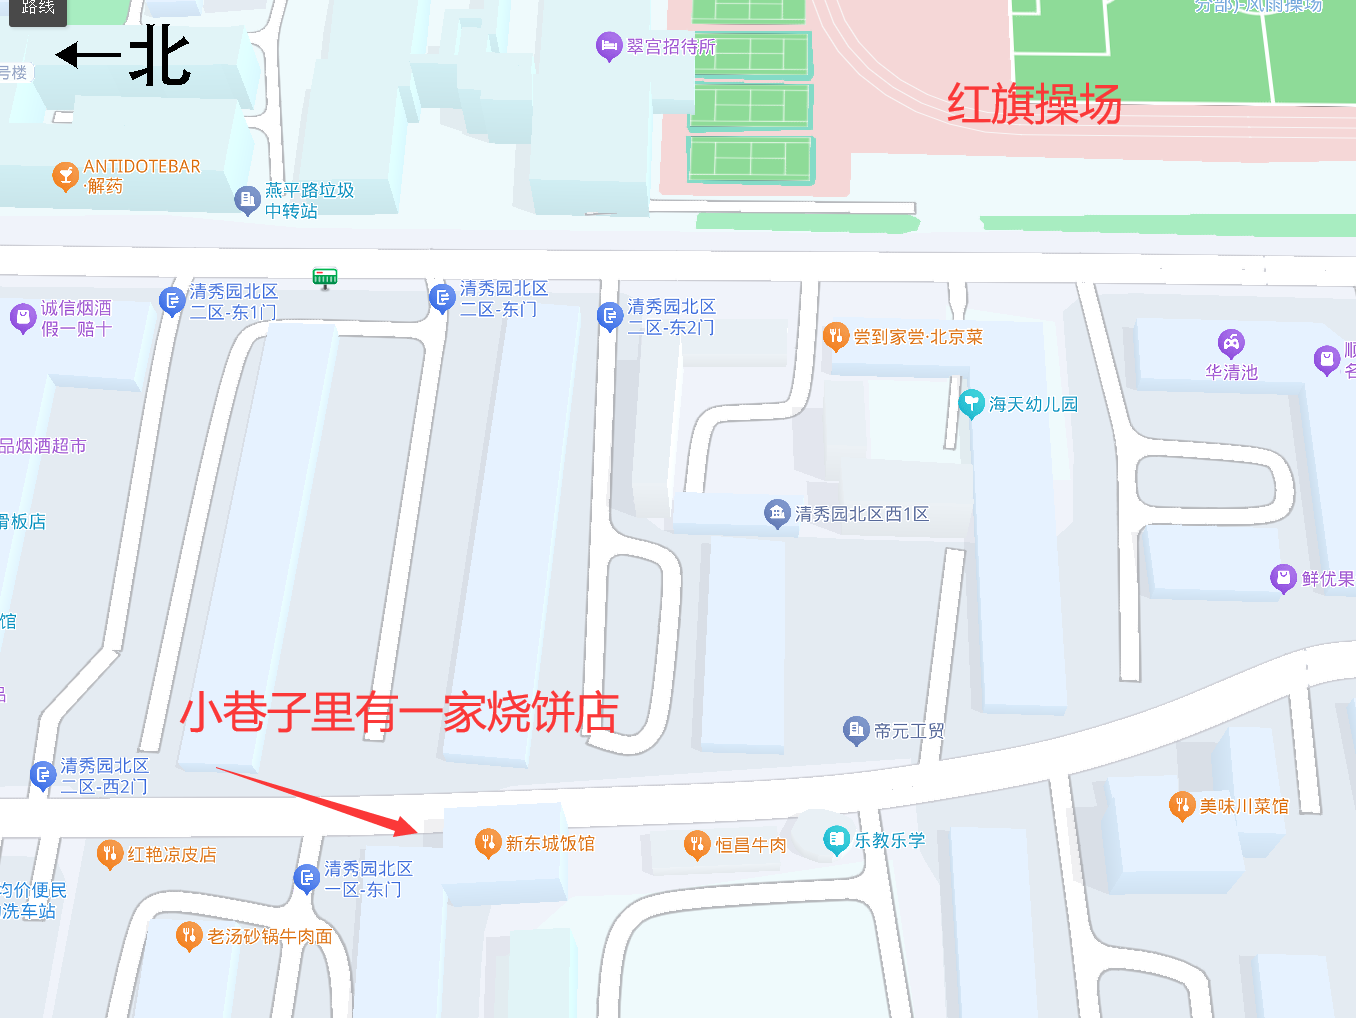
\includegraphics[width=0.8\textwidth]{pics/校外/清秀园/烧饼.png}
\end{figure}

\textbf{\subsubsection*{3. 啤酒超市}}
\addcontentsline{toc}{subsubsection}{3.2.3 \ 啤酒超市}
\begin{figure}[ht]
	\centering
	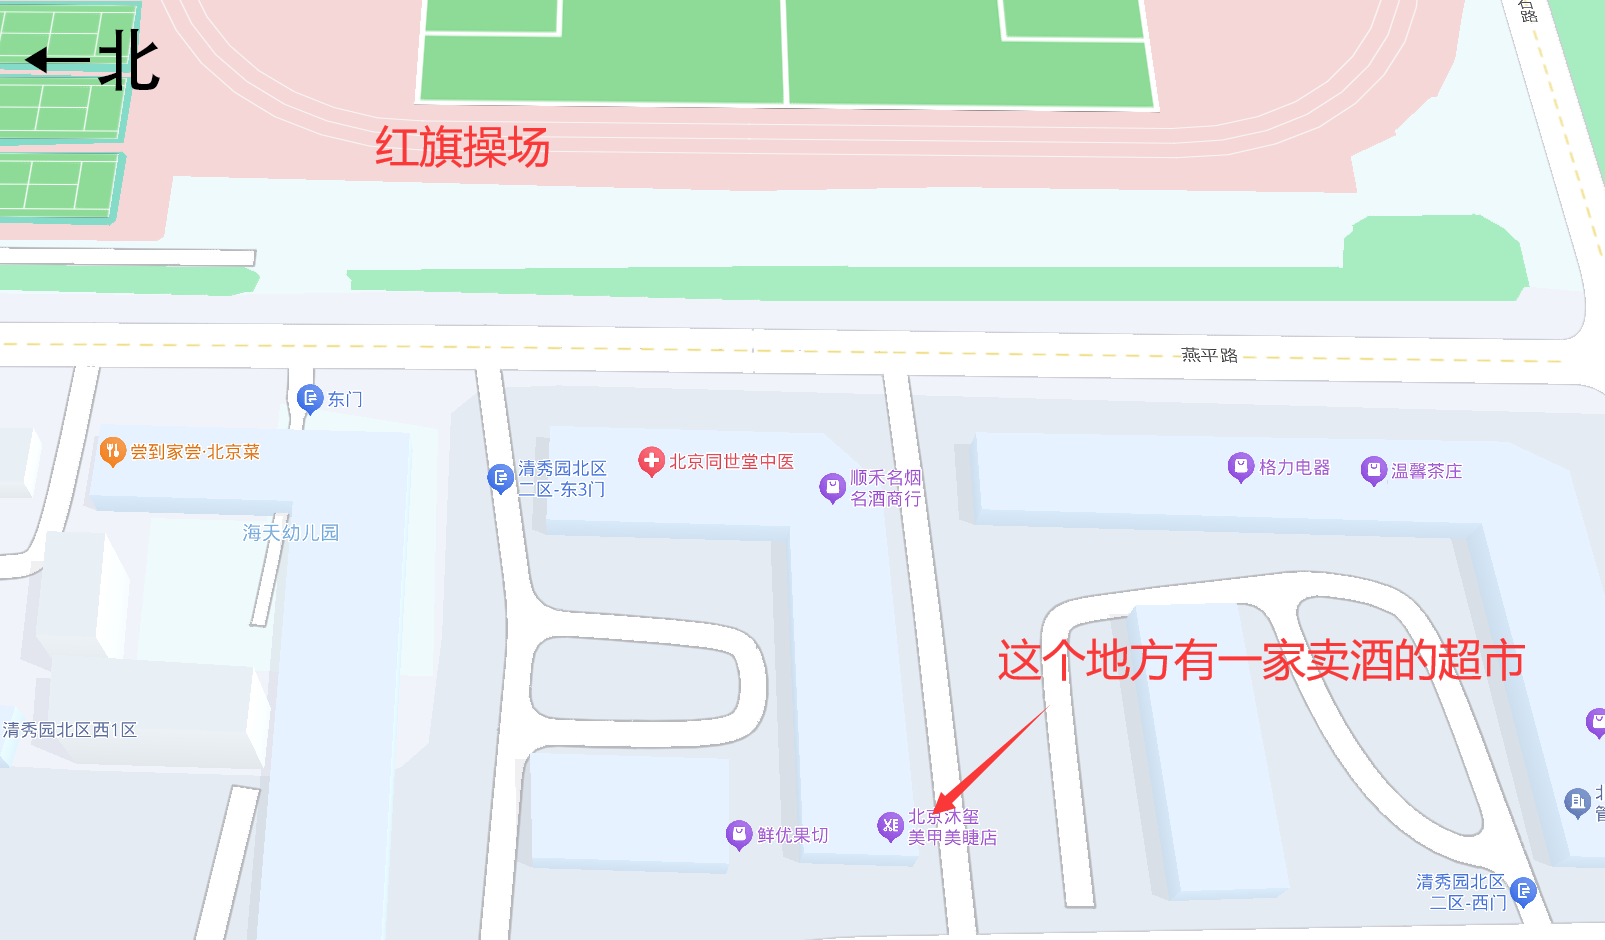
\includegraphics[width=0.8\textwidth]{pics/校外/清秀园/酒店.png}
\end{figure}
这家为什么要单独强调,因为卖的酒实在是太高级了,从4块到50块,可谓应有尽有,满足你对啤酒的99\%需求,无论是中国的,欧洲的,美国的,甚至印度的,俄罗斯的,没有你找不到,只有你想不到。我强推的有诱惑7(Tempt 7),像气泡甜水,很有意思;百威白啤,非常实惠又好喝的平价酒,还有上百种等待着同学们去探索。

\textbf{注:买完酒去川菜馆吃饭的时候喝100\%会感觉很撑,别问我为什么,问就是每次我都是这样,很奇怪。}

\textbf{\subsubsection*{4. 砂锅牛肉面}}
\addcontentsline{toc}{subsubsection}{3.2.4 \ 砂锅牛肉面}
\begin{figure}[ht]
	\centering
	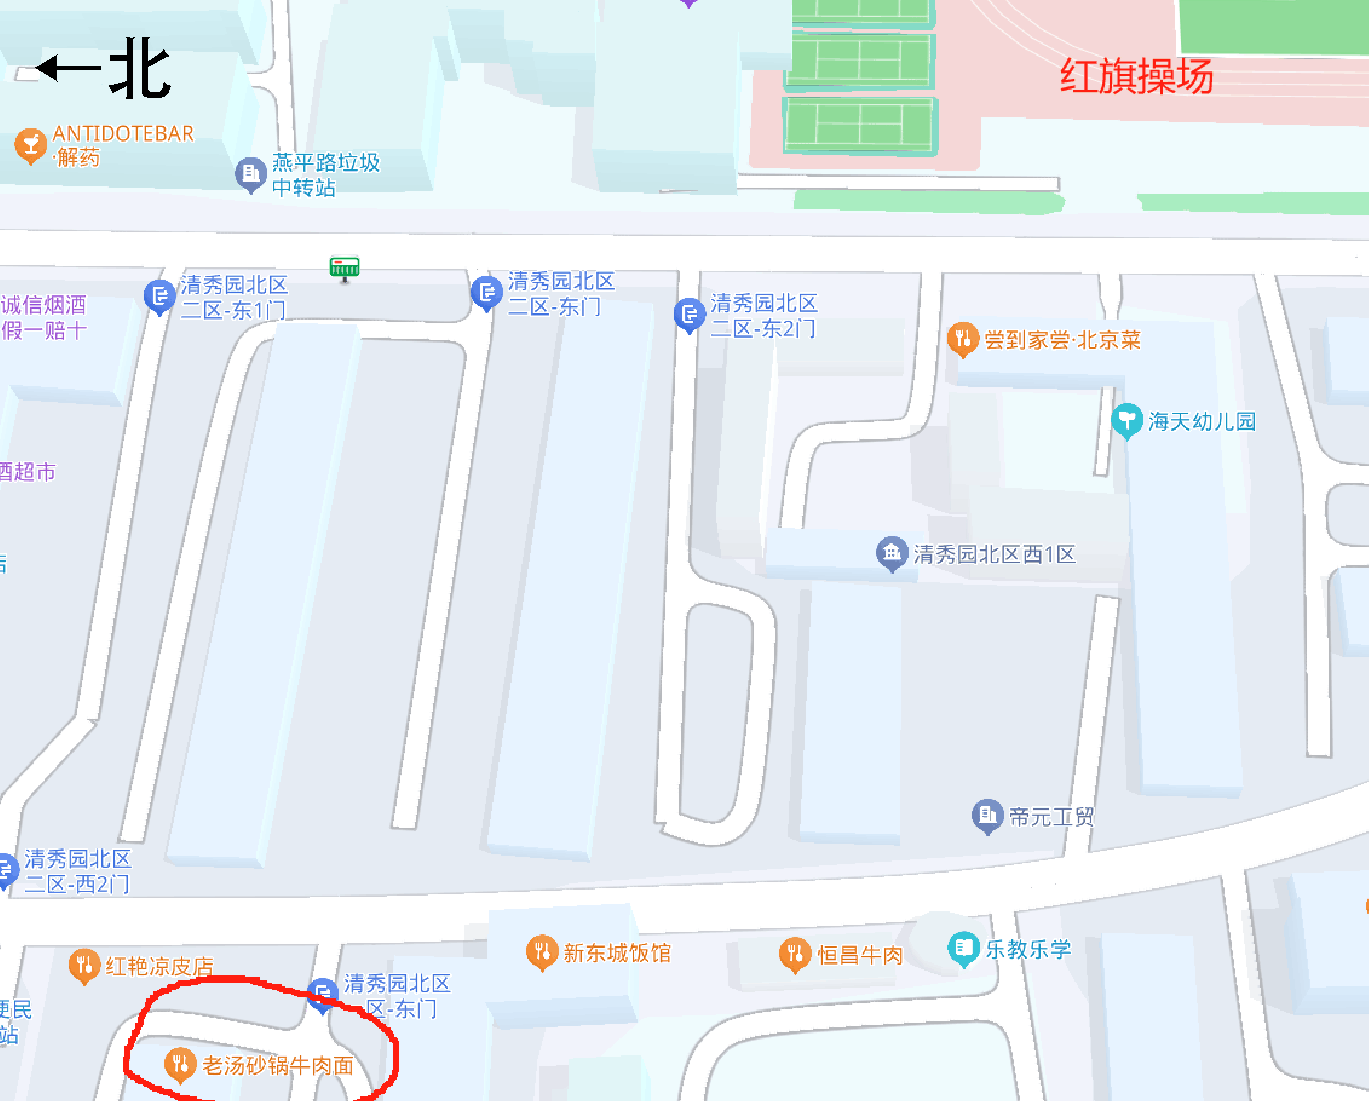
\includegraphics[width=0.8\textwidth]{pics/校外/清秀园/砂锅面.png}
\end{figure}
这家可能是作者在学校附近找到的唯一一家砂锅牛肉面,确实好吃,店面一直开到晚上十点。要注意的是,砂锅刚上来的时候特别烫,建议先放10分钟再吃,不然嘴被烫伤问题就大了。

\textbf{\subsubsection*{5. 尝到家尝(提供者:Silenchatter)}}
\addcontentsline{toc}{subsubsection}{3.2.5 \ 尝到家尝}
北平人家旗下北京菜系,经典菜鱼头泡饼可食(最好多几个人)。他们家也是附近为数不多可以点豆汁的店,请挑战自己。
\begin{figure}[ht]
	\centering
	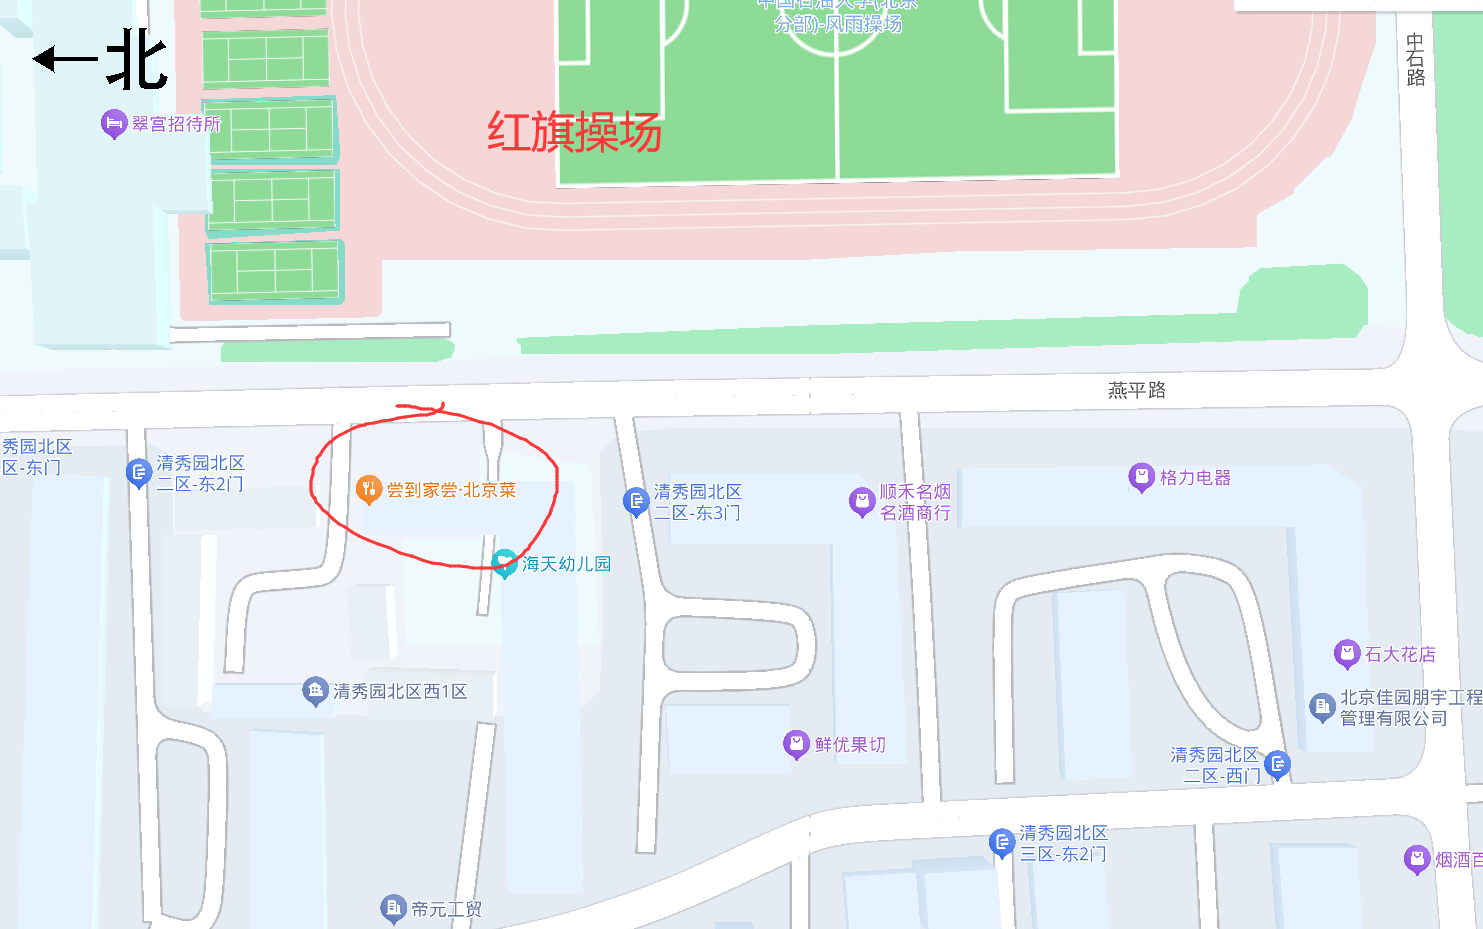
\includegraphics[width=0.8\textwidth]{pics/校外/清秀园/尝到家尝.png}
\end{figure}

\newpage
\textbf{\subsection*{三、润杰门口一条街}}
\addcontentsline{toc}{subsection}{3.3 \ 润杰门口一条街}
\fontsize{14pt}{16.8pt}\selectfont
\setlength{\parindent}{2em} % 设置首行缩进为2字符
炒饼,煎饼,夹馍等暂且不做评价,更新换代太快不便记录,而且口碑大家有目共睹。

\textbf{\subsubsection*{1. 川渝小厨(提供者:Ash)}}
\addcontentsline{toc}{subsubsection}{3.3.1 \ 川渝小厨}
\begin{figure}[ht]
	\centering
	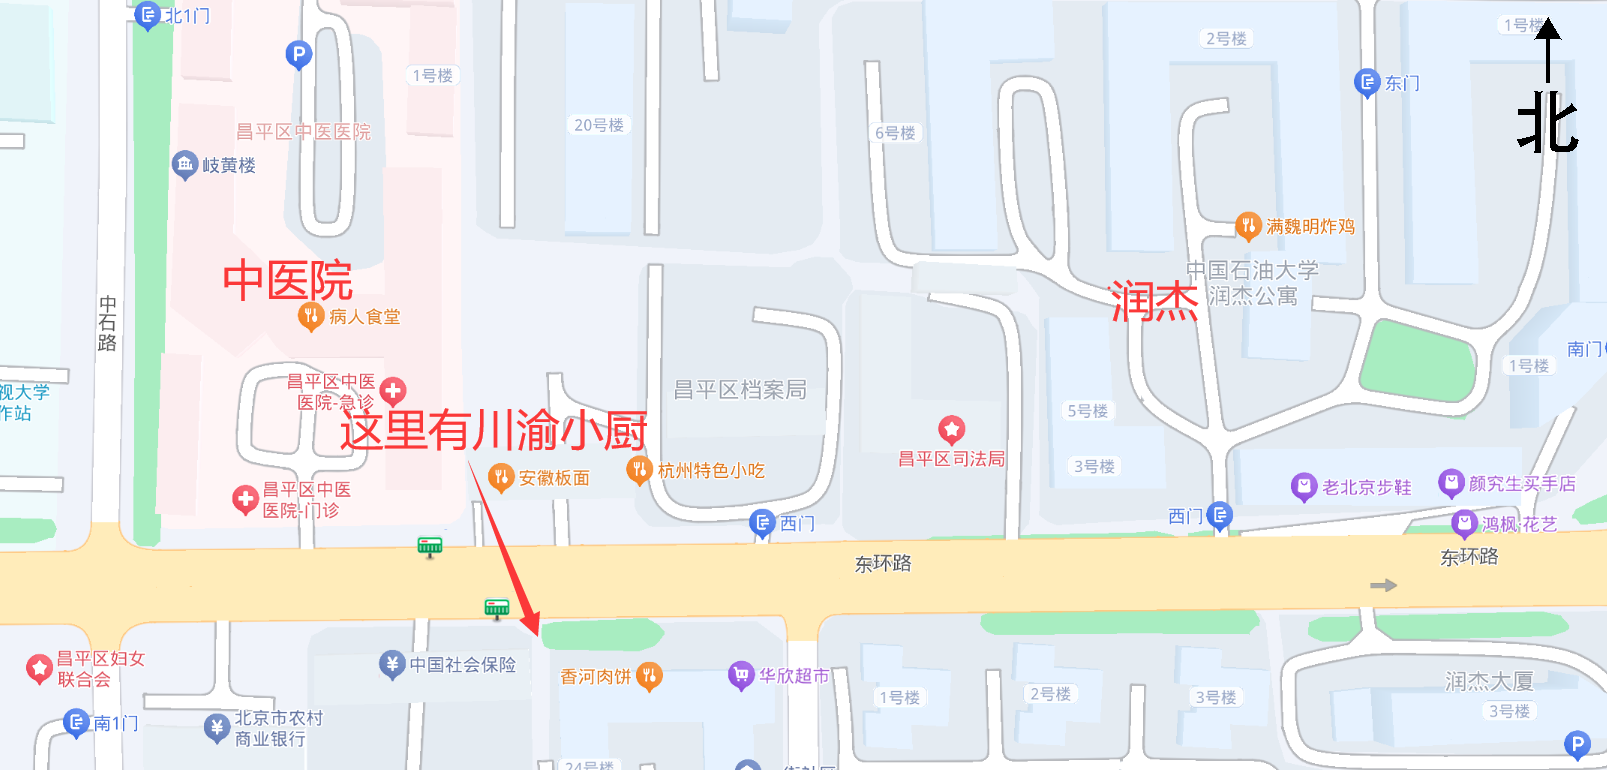
\includegraphics[width=0.7\textwidth]{pics/校外/润杰/川渝小厨.png}
\end{figure}
川渝小厨作为传说中的你校校外食堂广受好评,单人前往的时候有可以不限量添饭的各式盖饭,三两好友相聚的时候也可以点上几个炒菜。价格相当的亲民,一般情况下平均每顿饭20-30,这个价位就能吃饱了。说是川菜但是实际上并没有很辣,口味改良过,受众还是比较广的。推荐菜:水煮肉片,铁板日本豆腐,干锅土豆片。

\textbf{\subsubsection*{2. 哈尔滨麻辣烫}}
\addcontentsline{toc}{subsubsection}{3.3.2 \ 哈尔滨麻辣烫}
除一餐麻辣香锅外昌平第二便宜麻辣烫,除味道有些淡以外无任何缺点,老板娘人特别好,无脑冲就完事了!
\begin{figure}[ht]
	\centering
	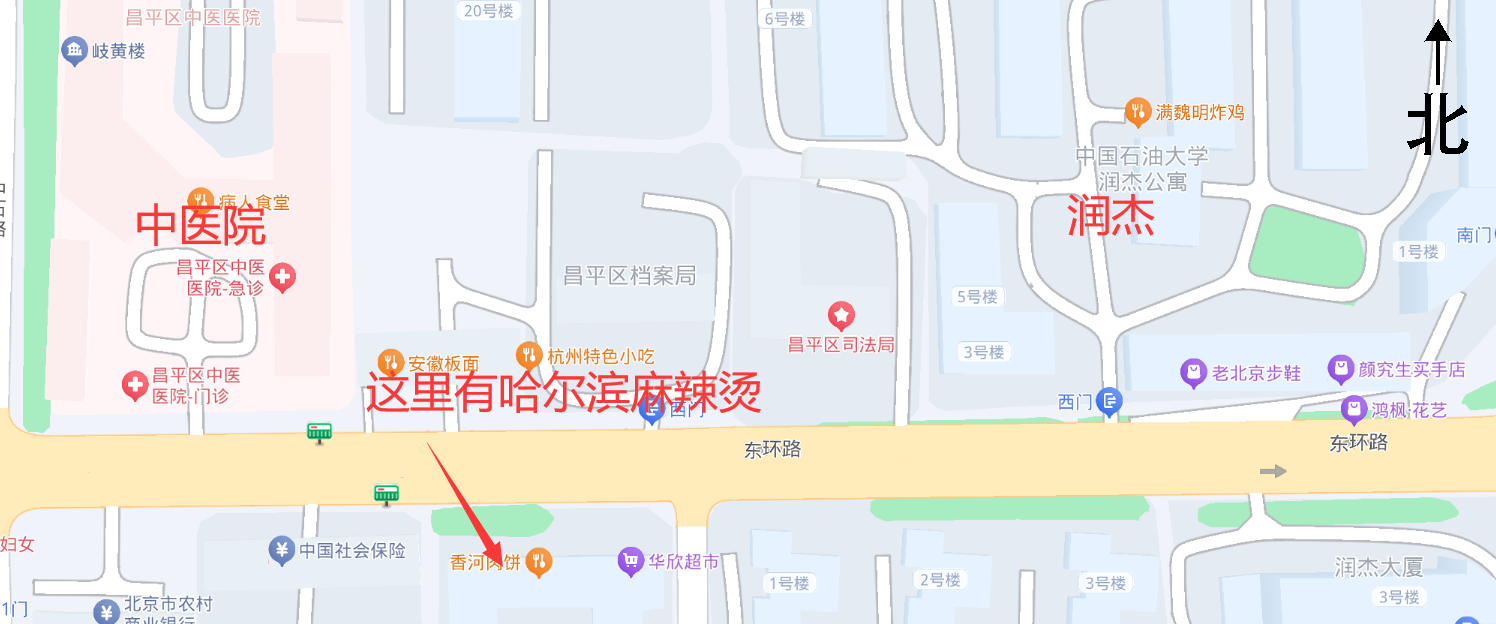
\includegraphics[width=0.7\textwidth]{pics/校外/润杰/哈尔滨麻辣烫.png}
\end{figure}


\newpage
\textbf{\subsection*{四、阳光商厦一条街}}
\addcontentsline{toc}{subsection}{3.4 \ 阳光商厦一条街}
\fontsize{14pt}{16.8pt}\selectfont
\setlength{\parindent}{2em} % 设置首行缩进为2字符
政法旁边,国泰对面,清秀园后面,就是著名的阳光商厦,周围东西不少,主要推荐以下。

\textbf{\subsubsection*{1. 好伦哥}}
\addcontentsline{toc}{subsubsection}{3.4.1 \ 好伦哥}
\begin{figure}[ht]
	\centering
	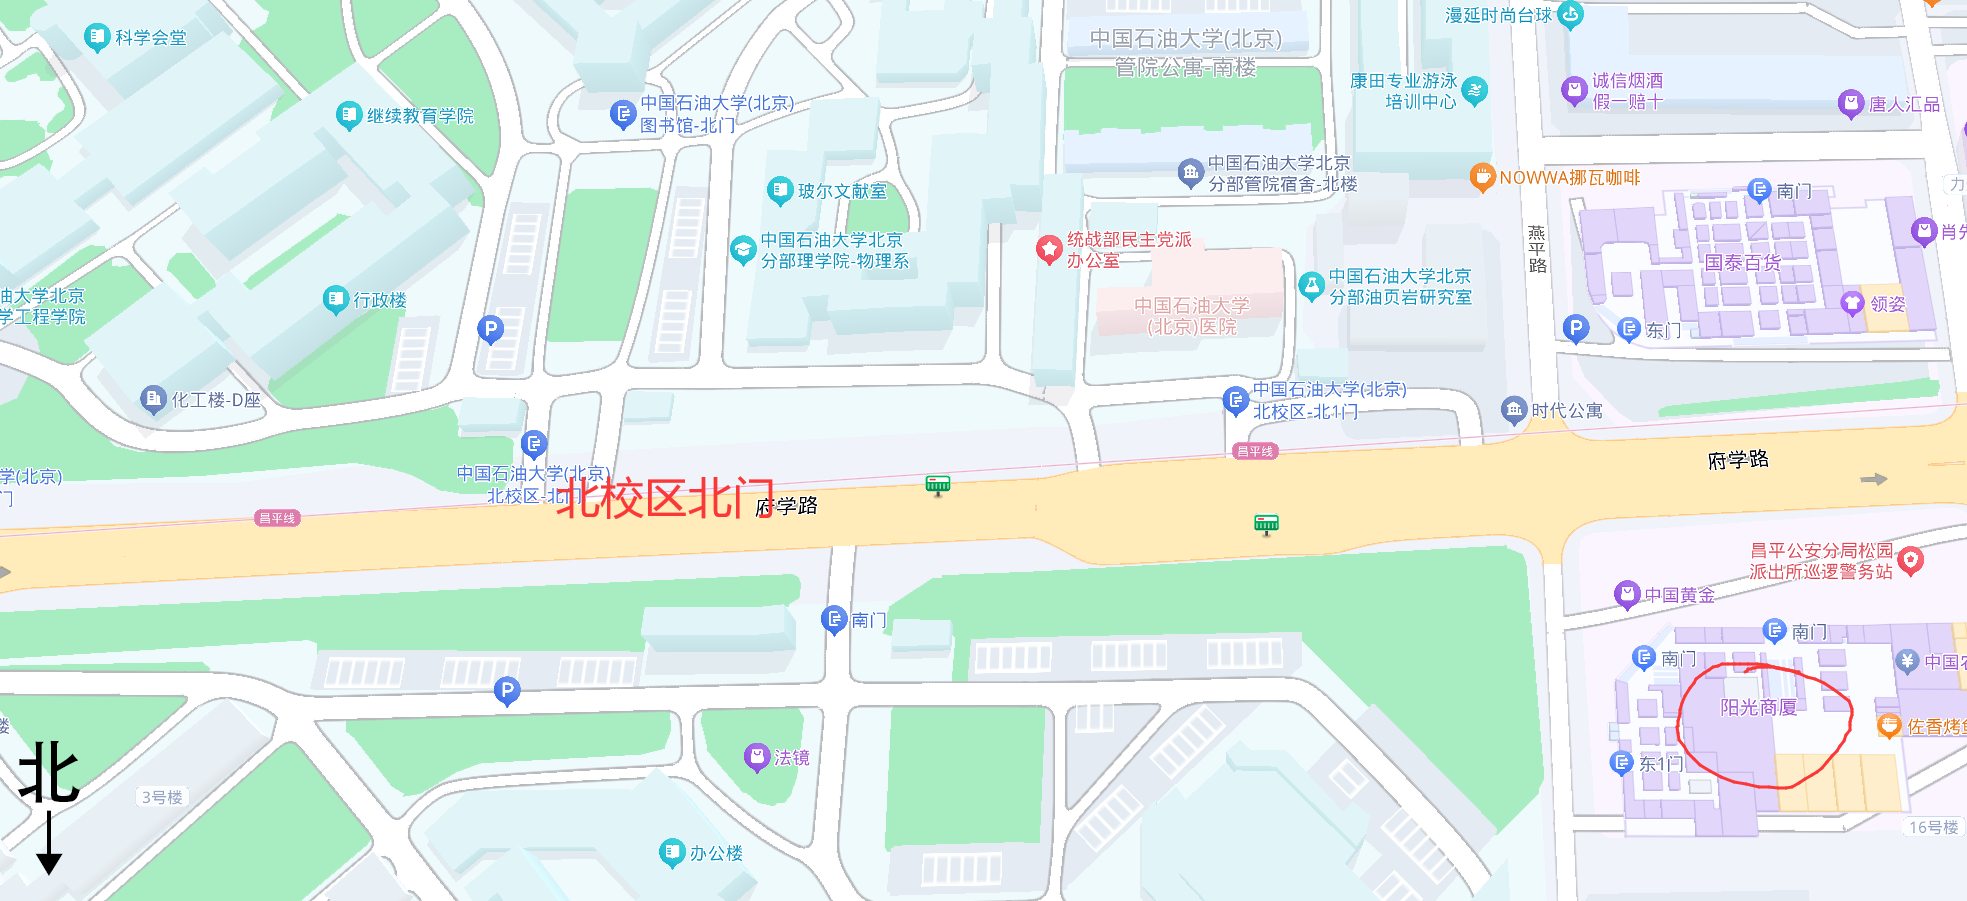
\includegraphics[width=0.75\textwidth]{pics/校外/阳光商厦/好伦哥.png}
\end{figure}
好伦哥在阳光商厦顶楼,个人感觉好像阳光商厦除了好伦哥别的店都跑路了,这也证实了好伦哥的强大。美团学生券80-90不等,工作日稍便宜点。中午11点晚上5点开餐,如果你来晚了,有可能排上百号人的队,这个时候就退了走人吧,作者亲身经历是一小时排了60号,排到结束都排不到,火爆的难以想象。进去建议先拿牛排烤鸭,一次拿一块,可以排两次队,等下一波(20分钟左右)可以继续排。
\textbf{\subsubsection*{2. 地下超市}}
\addcontentsline{toc}{subsubsection}{3.4.2 \ 地下超市}
\begin{figure}[ht]
	\centering
	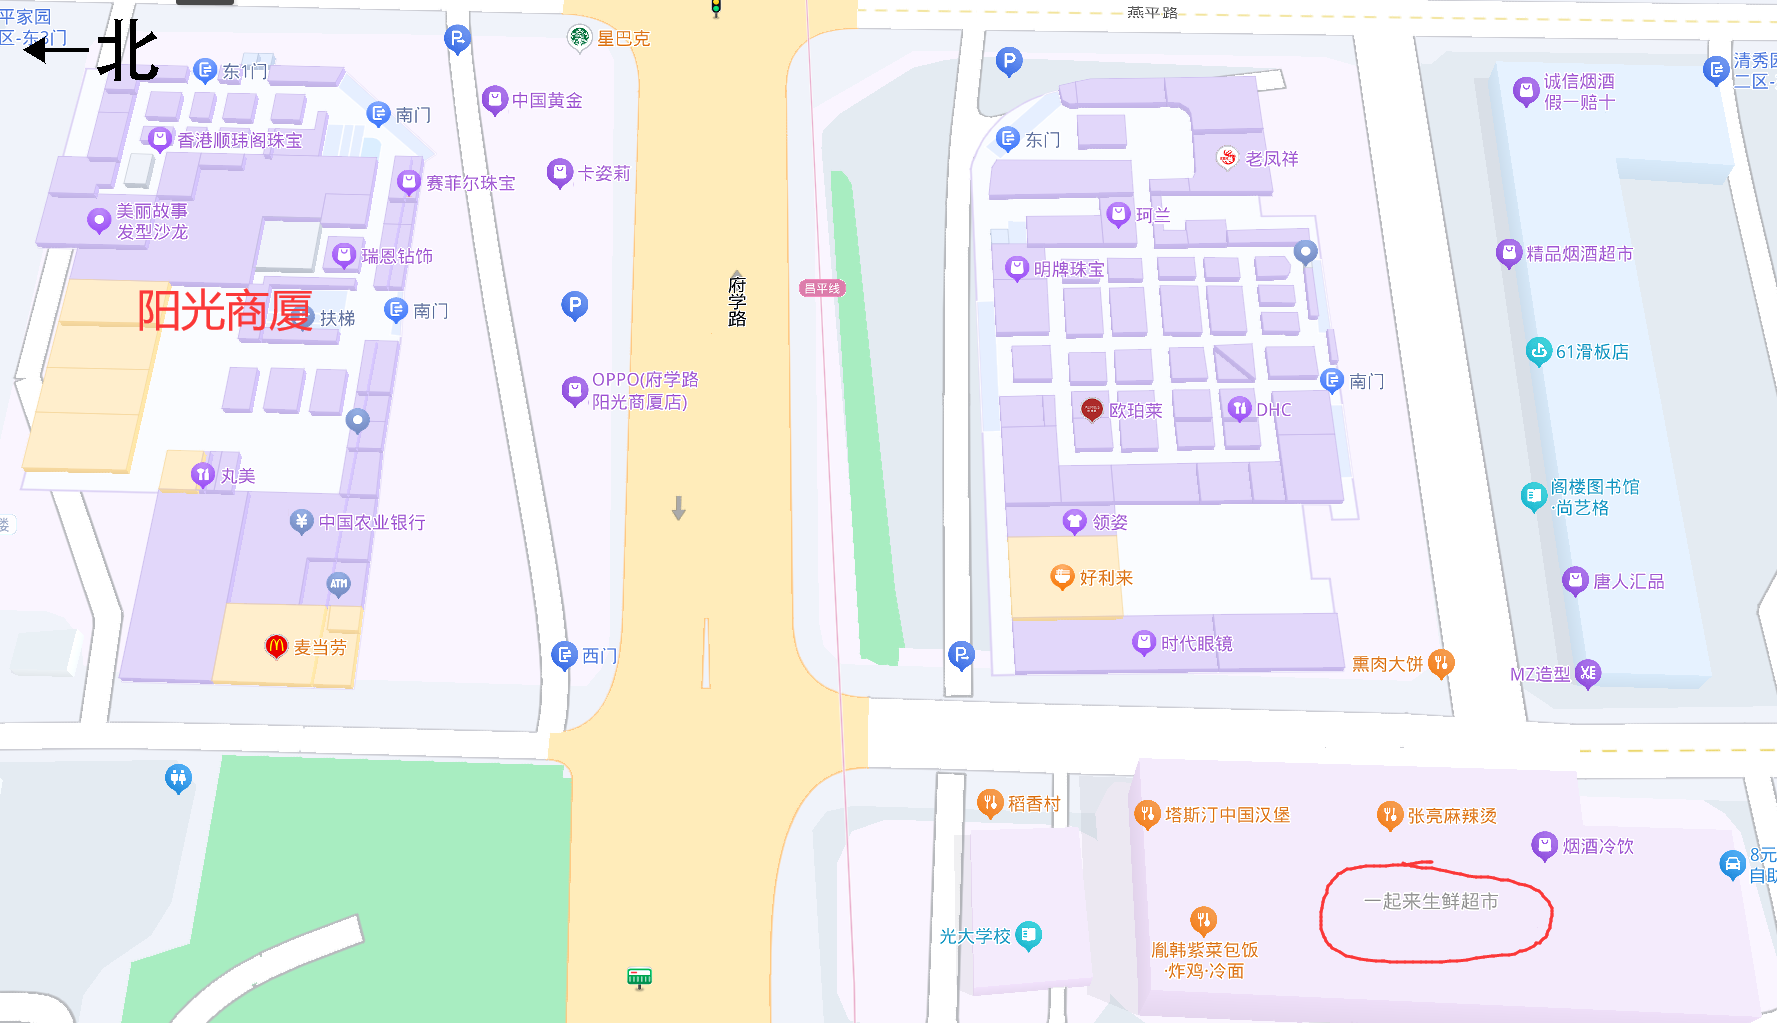
\includegraphics[width=0.6\textwidth]{pics/校外/阳光商厦/生鲜超市.png}
\end{figure}这个地下超市卖的东西往往比南校园闸机口一条街的各种店更便宜,尤其是水果。举个例子来说,今年夏天的无子麒麟瓜2.5一斤,半个8块左右。超市入口在图中稻香村的位置。缺点是地下稍微有点热,排队有时候比较长。另外,如果你买瓜的话,结完账有一个帮你切完装盒的窗口,还是非常方便的。

\textbf{\subsubsection*{3. 达美乐}}
\addcontentsline{toc}{subsubsection}{3.4.3 \ 达美乐}
\begin{figure}[ht]
	\centering
	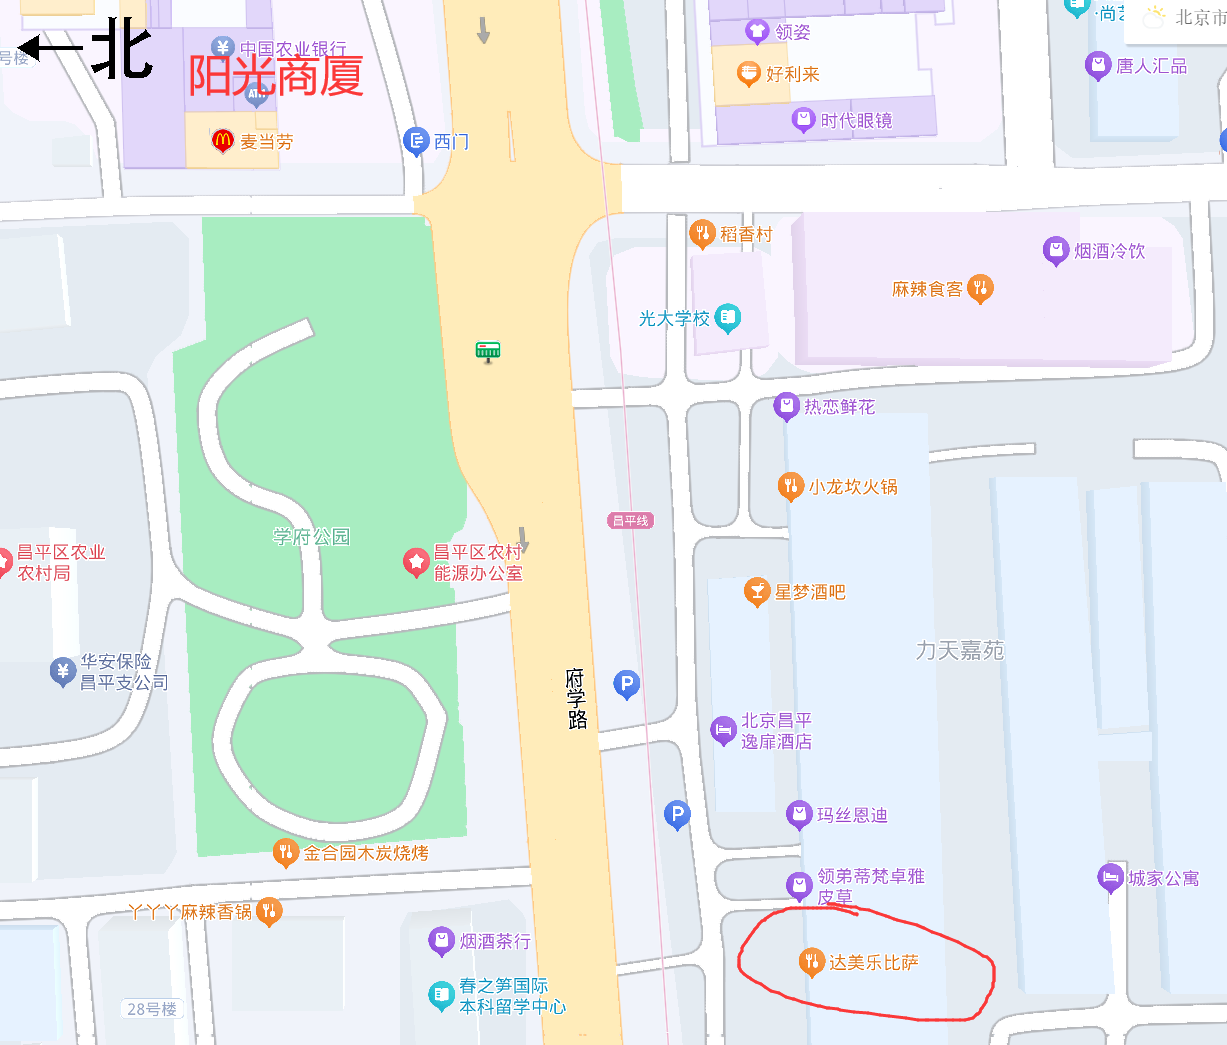
\includegraphics[width=0.6\textwidth]{pics/校外/阳光商厦/达美乐.png}
\end{figure}
收录达美乐的原因是它不定期有披萨买一送一活动,否则性价比不太高,建议等活动的时候来,相当于一张披萨才20左右,还是很爽的。

\textbf{\subsubsection*{4. 麦当劳(提供者:Ash)}}
\addcontentsline{toc}{subsubsection}{3.4.4 \ 麦当劳}
\begin{figure}[ht]
	\centering
	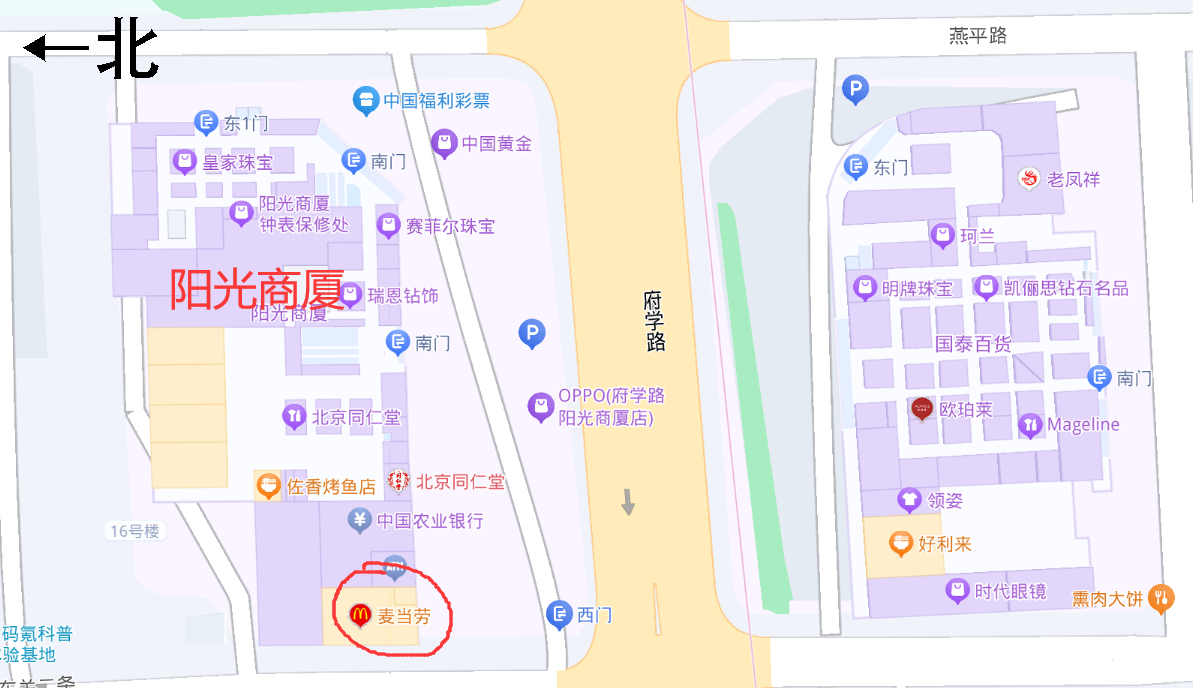
\includegraphics[width=0.7\textwidth]{pics/校外/阳光商厦/麦当劳.png}
\end{figure}
麦当劳作为十里八乡出名的老北京特色美食,优越性体现在全年都有的穷鬼套餐1+1以及作为一代人心目中的经典巨无霸和薯条。值得一提的是麦当劳的甜品也十分值得称道,在平级的快餐店中甜筒质量遥遥领先。

另外,支付宝学生认证可以领劵(白嫖),麦当劳App学生认证可以获得优惠价麦金会员。


\textbf{\subsubsection*{5. 汉堡王(提供者:Ash)}}
\addcontentsline{toc}{subsubsection}{3.4.5 \ 汉堡王}
常言道:英国唯一的国王就是汉堡王。皇堡拥有连锁快餐店中难以寻得的新鲜洋葱圈和西红柿片,极大程度丰富了口感。不过平时较贵,仅推荐周三的国王日活动特价套餐。
\begin{figure}[ht]
	\centering
	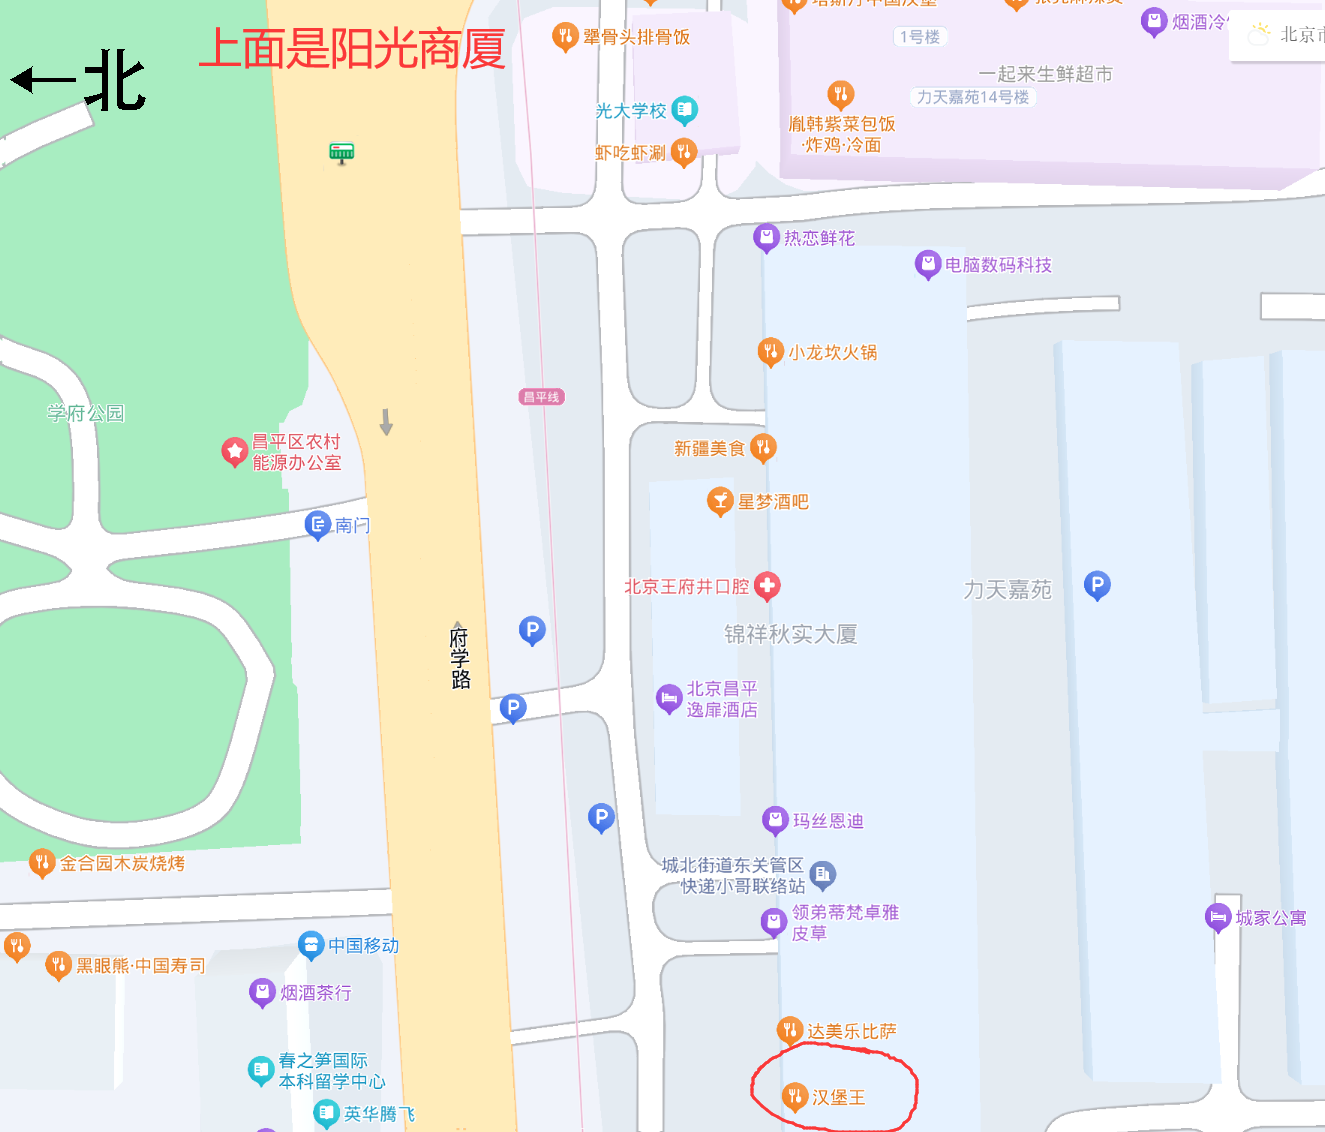
\includegraphics[width=0.5\textwidth]{pics/校外/阳光商厦/汉堡王.png}
\end{figure}

\textbf{\subsubsection*{6. 千叶寿司(提供者:Silenchatter)}}
\addcontentsline{toc}{subsubsection}{3.4.6 \ 千叶寿司}
价格实惠性价比高,手艺还不错。推荐天妇罗虾以及招牌系列寿司。
\begin{figure}[ht]
	\centering
	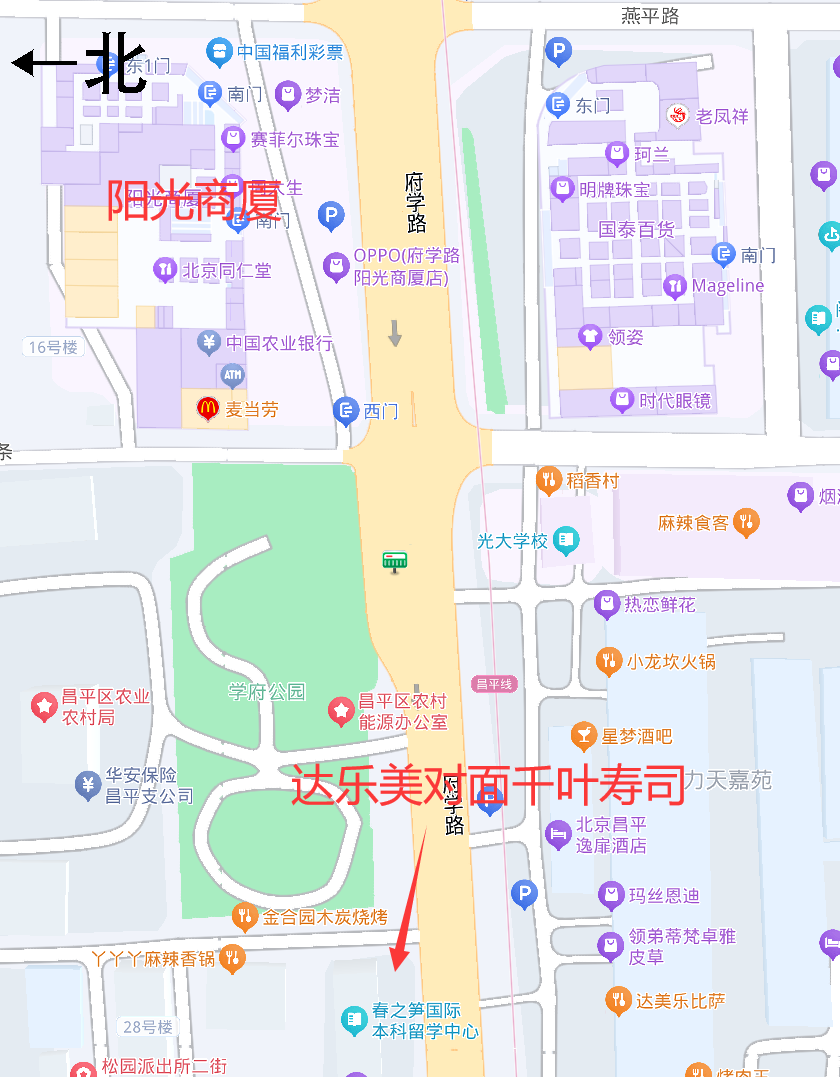
\includegraphics[width=0.45\textwidth]{pics/校外/阳光商厦/千叶寿司.png}
\end{figure}
\textbf{\subsubsection*{7. 云三哚(提供者:Silenchatter)}}
\addcontentsline{toc}{subsubsection}{3.4.7 \ 云三哚}
位置有点偏,主打云南风味米线。价格稍微有点点高,但是米线确实正宗。
\begin{figure}[ht]
	\centering
	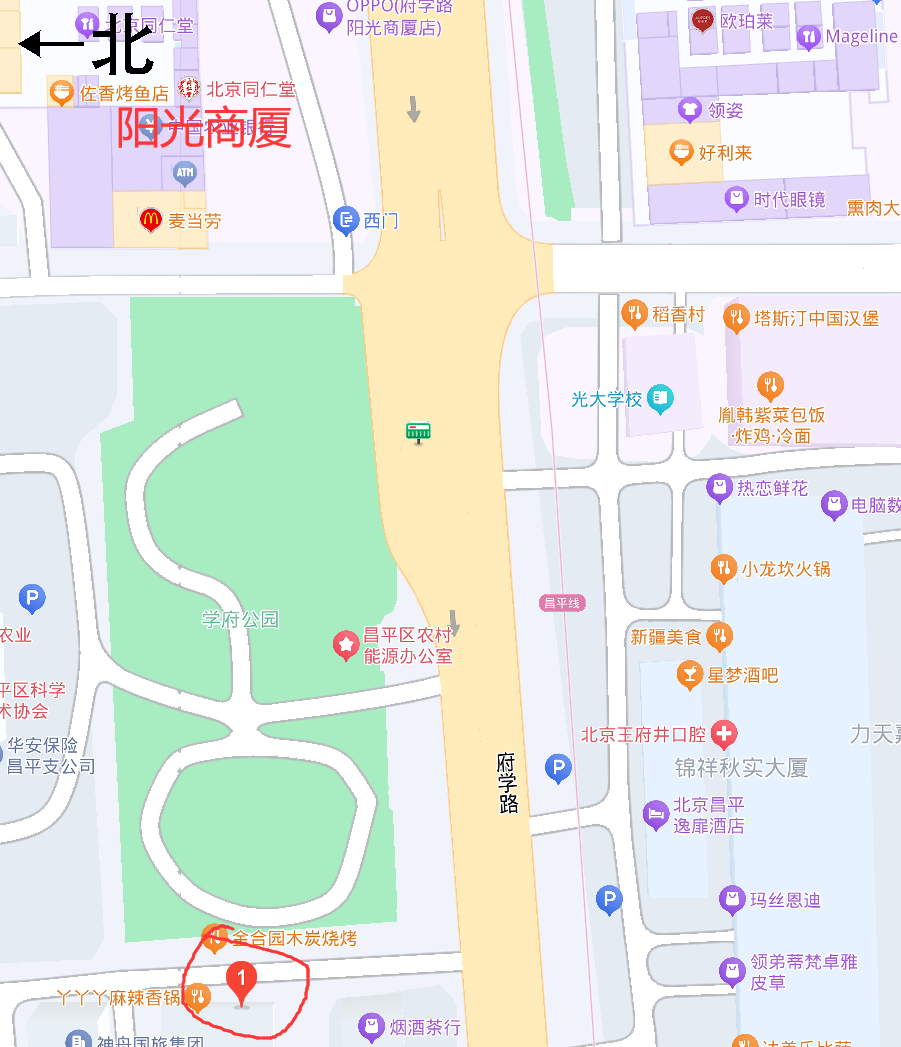
\includegraphics[width=0.45\textwidth]{pics/校外/阳光商厦/云三哚.png}
\end{figure}

\textbf{\subsubsection*{8. 虾吃虾涮/王婆大虾(提供者:Silenchatter)}}
\addcontentsline{toc}{subsubsection}{3.4.8 \ 虾吃虾涮/王婆大虾}
\begin{figure}[ht]
	\centering
	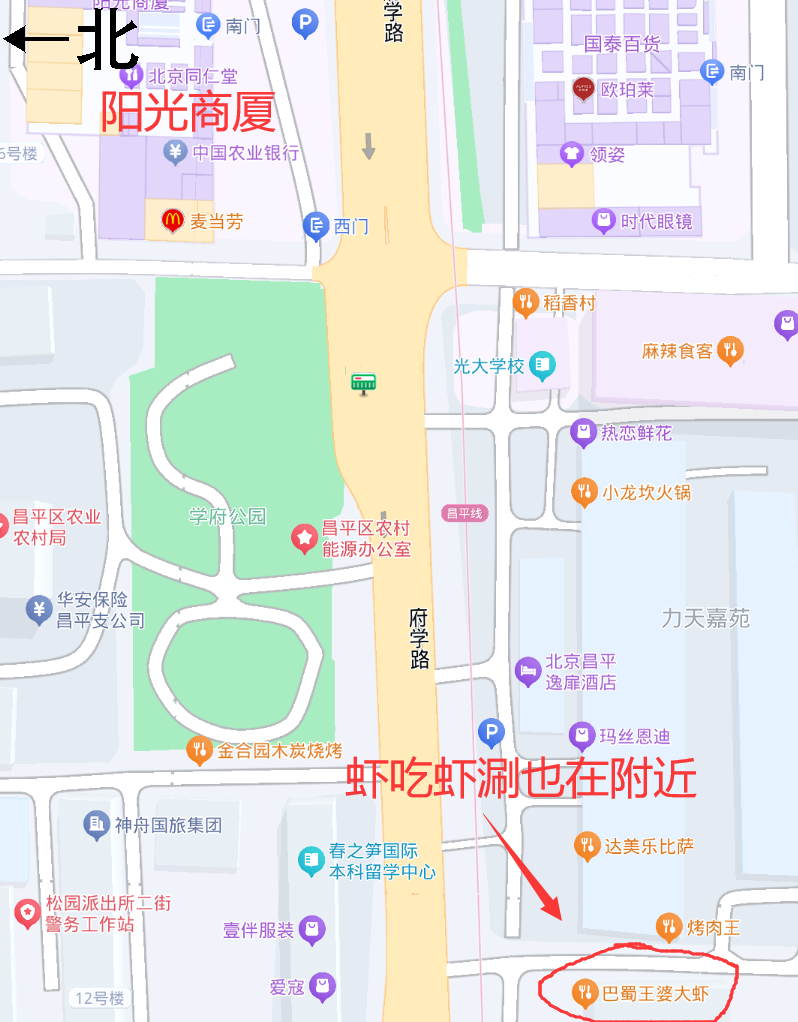
\includegraphics[width=0.45\textwidth]{pics/校外/阳光商厦/王婆大虾.png}
\end{figure}
虾火锅。两家差不多,王婆人均高10,套餐适合团建。本人口味偏重,喜欢一口气把虾剥完后放回锅内吸汤,可以根据个人喜好吃。 

\newpage
\textbf{\subsection*{五、东校区一条街}}
\addcontentsline{toc}{subsection}{3.5 \ 东校区一条街}
\fontsize{14pt}{16.8pt}\selectfont
\setlength{\parindent}{2em} % 设置首行缩进为2字符
对于本科同学来说,东校区去的很少,对那一条街自然也就不甚了解。作者也尝试了一些,以下是一些比较好的店。

\textbf{\subsubsection*{1. 螺狮粉}}
\addcontentsline{toc}{subsubsection}{3.5.1 \ 螺狮粉}
\begin{figure}[ht]
	\centering
	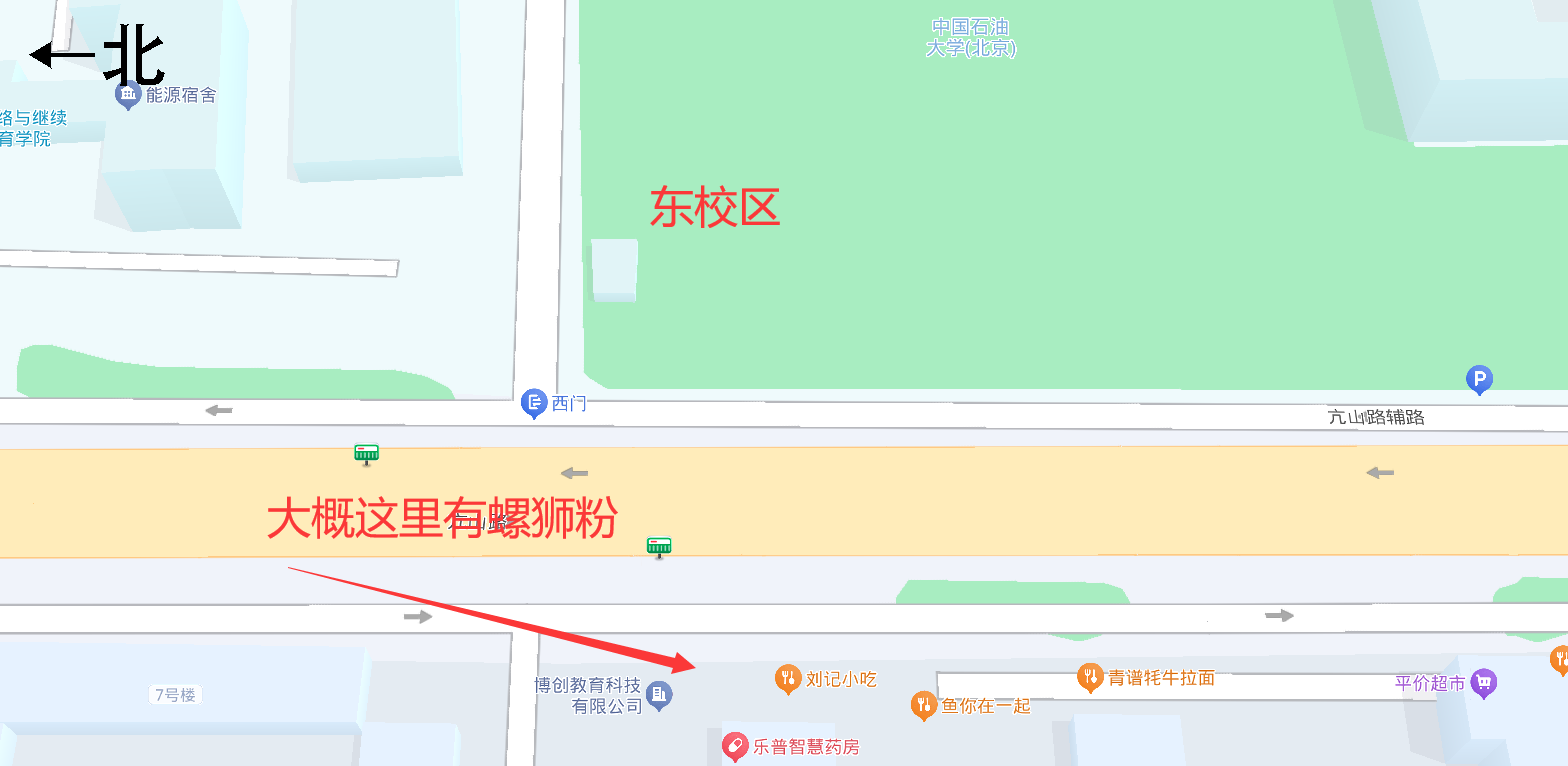
\includegraphics[width=0.73\textwidth]{pics/校外/东校/螺狮粉.png}
\end{figure}
不知道是不是我吃的少的缘故,我觉得螺狮粉很辣,一般情况下我点中辣就是极限了,大约等于一餐四楼的麻辣香锅特辣。螺狮粉好吃就不用多说了,17块钱左右,政法对面也有一家,有点远,价格差不多,因此我就只写了这一家。

\textbf{\subsubsection*{2. 板面}}
\addcontentsline{toc}{subsubsection}{3.5.2 \ 板面}

板面,近来可好?是否寝食安定?故乡的花一如往日般灿烂。不知你何时归来再于城下踏青赏花。此刻夜寝未久,楼外寒随雨起,雷藏云中,花随风落。山川异域,不知你身边是怎样的风景,是否双燕齐飞,春江水暖?有没有好好留意呢?风月同天,不知你身边是怎样的气象,是否像故乡般云烟缭绕,春雨润物?一种相思两处闲愁,幸好,夜不能寐孤寂落寞之时能看到你发的视频,得以慰藉。大抵你也是想我的,深感宠幸,唯望锻炼吉祥如意,武运昌隆,待来年春回,能共你一同赏花看海,诉说衷情。

咳咳,原谅我的发癫。众所周知正宗安徽板面在河北,作为一个河北人,看到板面就走不动路也是正常的。我的吃法是大碗宽板面加面,16块(老板肯定认识我了)。
\begin{figure}[ht]
	\centering
	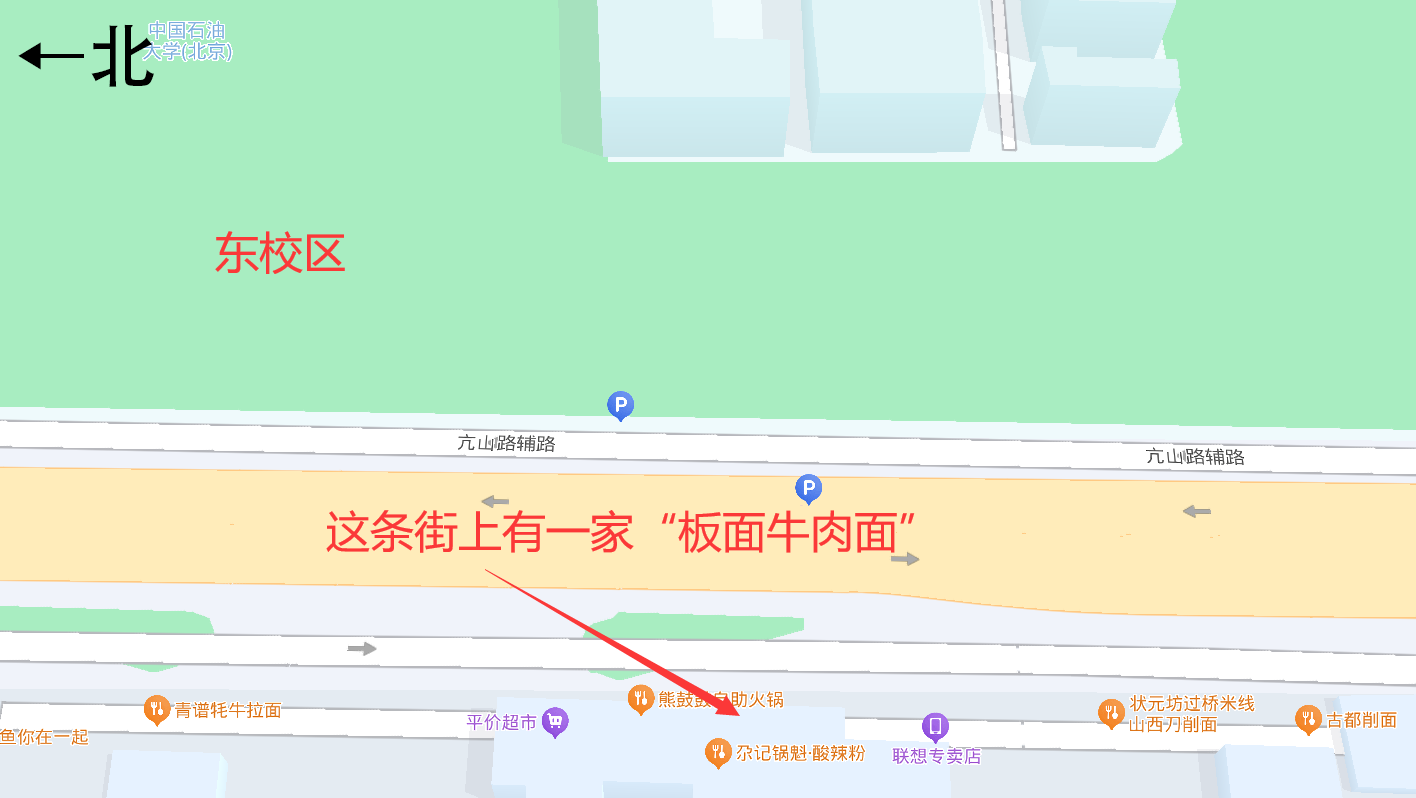
\includegraphics[width=0.75\textwidth]{pics/校外/东校/板面.png}
\end{figure}

\textbf{\subsubsection*{3. 晋大碗/人之初拉面(提供者:Silenchatter)}}
\addcontentsline{toc}{subsubsection}{3.5.3 \ 晋大碗/人之初拉面}
\begin{figure}[ht]
	\centering
	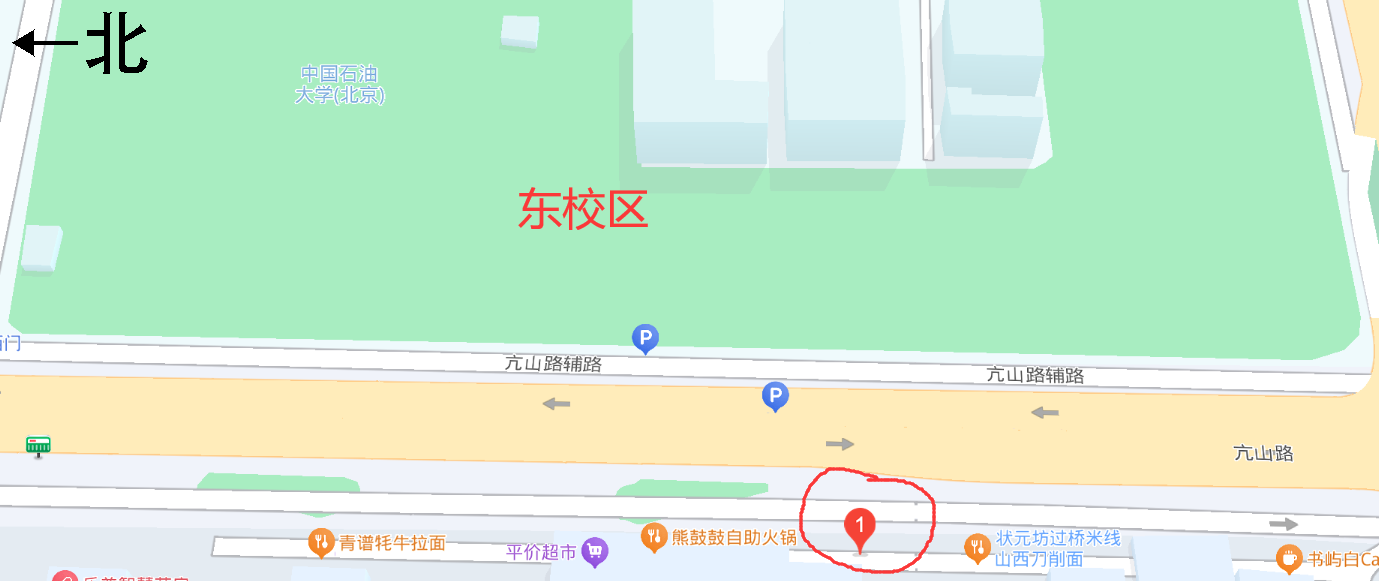
\includegraphics[width=0.73\textwidth]{pics/校外/东校/人之初.png}
\end{figure}
和板面并列为三家活了很久的面馆。作为爱吃面的北方人,学校食堂的面又比较一言难尽,这三家面确实能满足大部分人的需求 。

\textbf{\subsubsection*{4. 京东肉饼(提供者:Silenchatter)}}
\addcontentsline{toc}{subsubsection}{3.5.4 \ 京东肉饼}
\begin{figure}[ht]
	\centering
	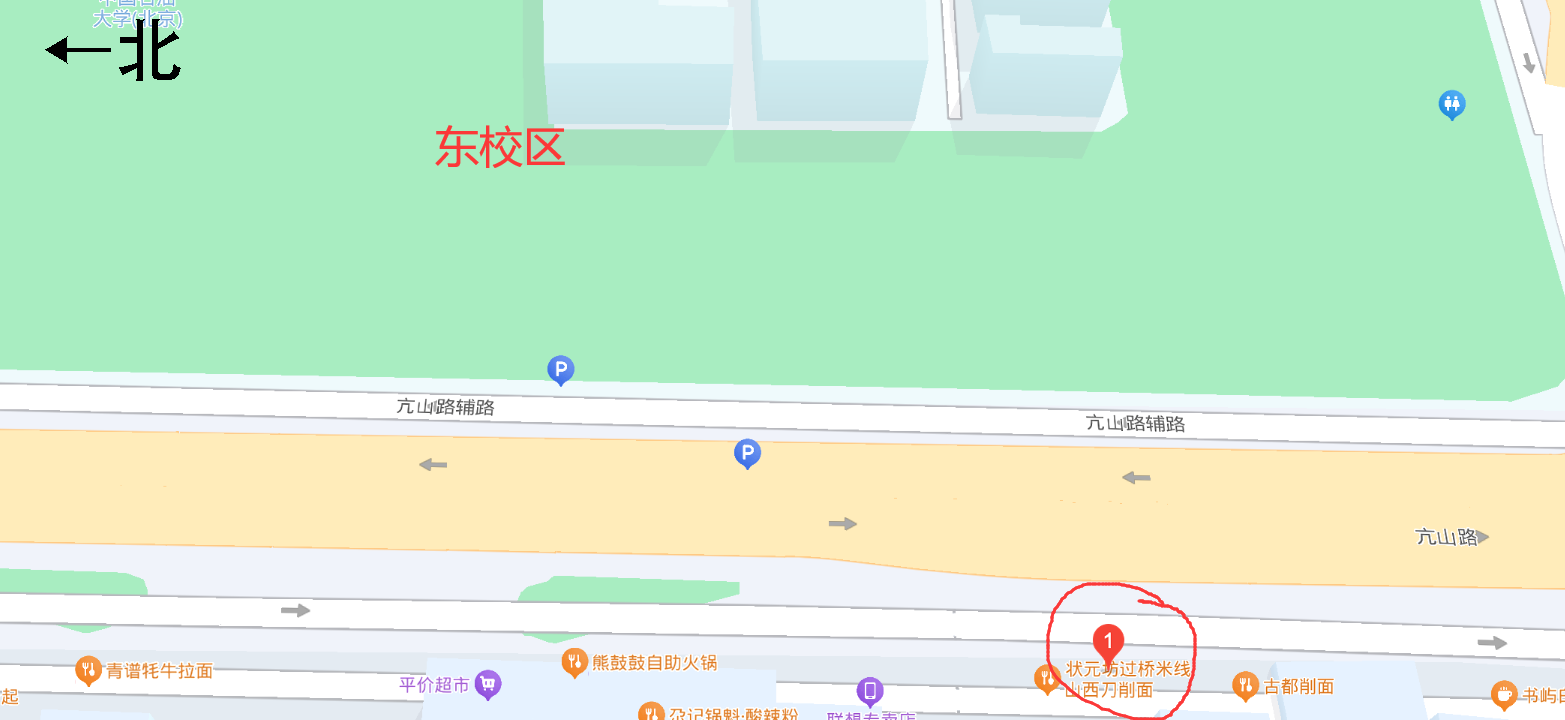
\includegraphics[width=0.73\textwidth]{pics/校外/东校/京东肉饼.png}
\end{figure}
适合三五好友小聚的店。人均四五十,可以点几个菜就着他们家的肉饼吃(每次都会误判食量以至于最后几块肉饼需要用石头剪刀布决定到底哪个撑的不行的人吃)。

\textbf{\subsubsection*{5. 段记肉夹馍(提供者:Silenchatter)}}
\addcontentsline{toc}{subsubsection}{3.5.5 \ 段记肉夹馍}
\begin{figure}[ht]
	\centering
	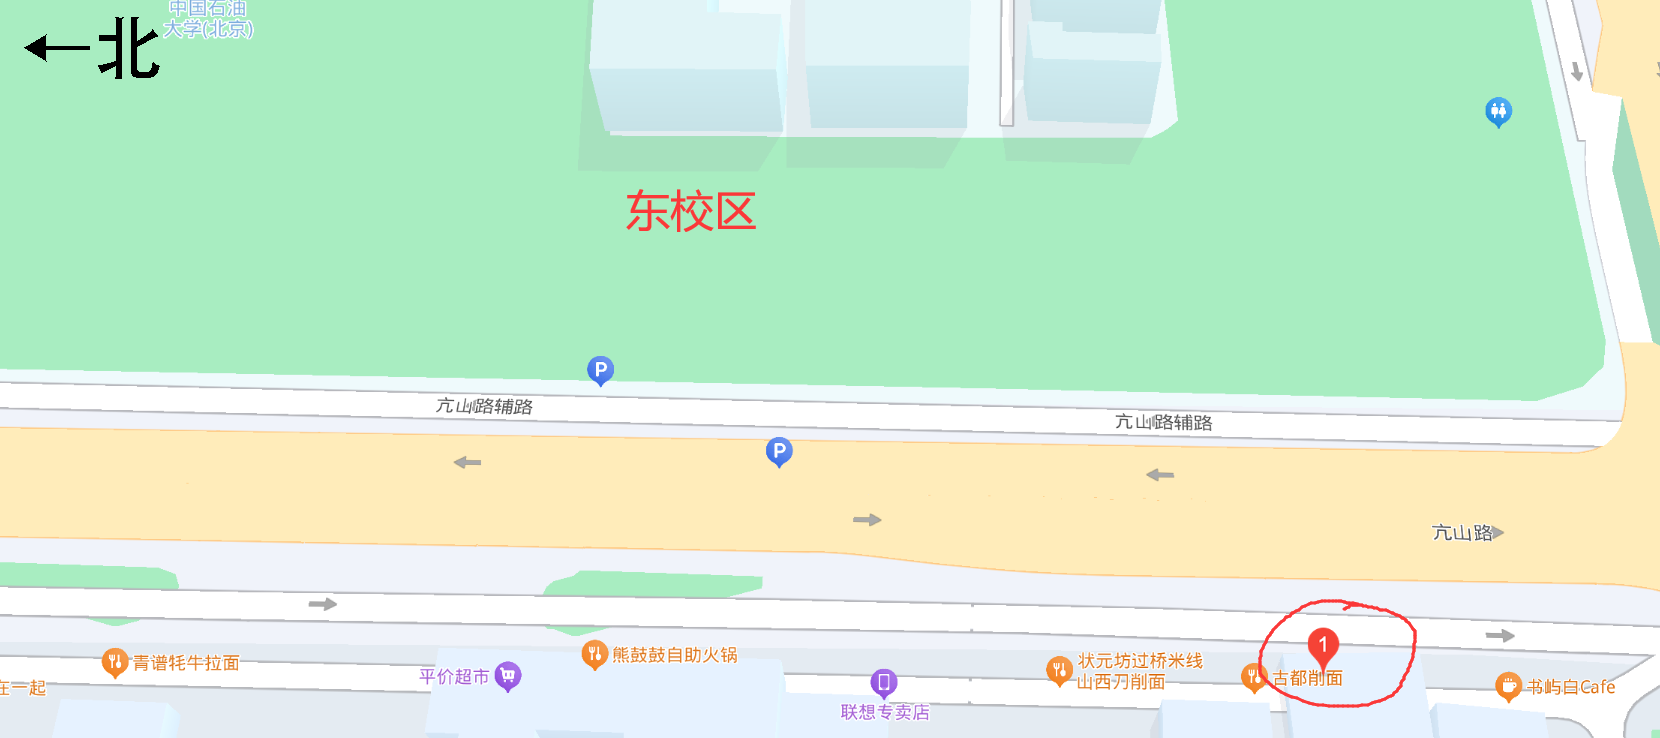
\includegraphics[width=0.73\textwidth]{pics/校外/东校/肉夹馍.png}
\end{figure}
一样适合三五好友小聚。肉夹馍算是做的比较好吃(陕西室友认同) 。

\textbf{\subsubsection*{6. 驴肉火烧(提供者:Silenchatter)}}
\addcontentsline{toc}{subsubsection}{3.5.6 \ 驴肉火烧}
\newpage
\begin{figure}[ht]
	\centering
	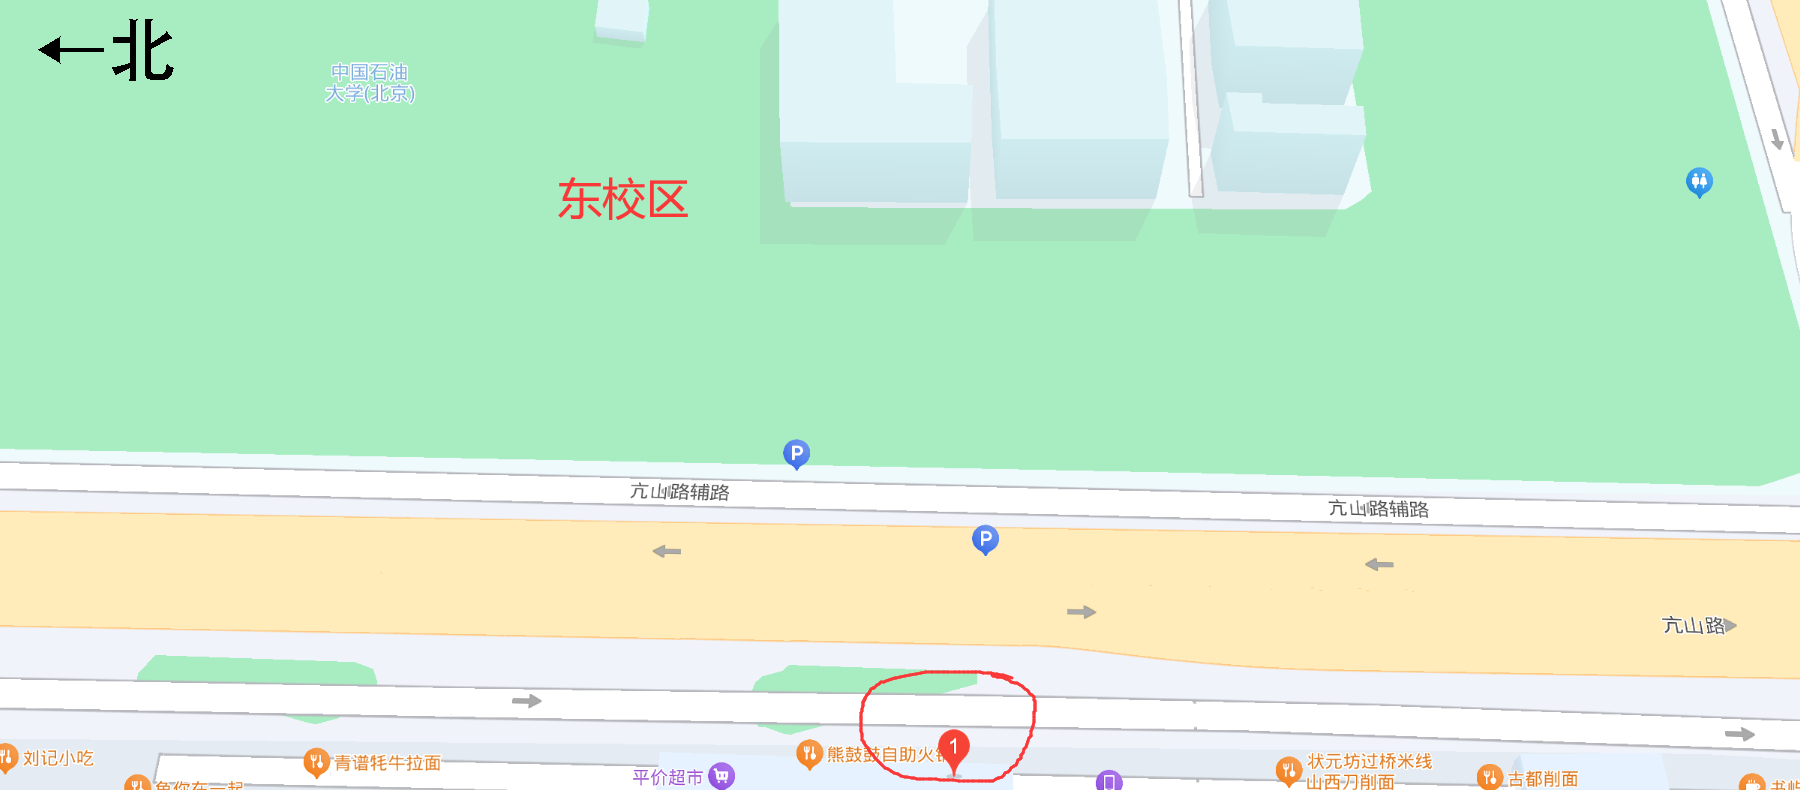
\includegraphics[width=0.73\textwidth]{pics/校外/东校/驴肉火烧.png}
\end{figure}
天上龙肉地上驴肉。不管你是不是河间/保定人,都要试一试驴肉火烧(学校附近的基本上都是河间驴肉火烧,本人也是河间派,吃驴肉加焖子火烧真的无敌),再来一碗驴杂汤,美滋滋。

\newpage
\textbf{\subsection*{六、悦荟}}
\addcontentsline{toc}{subsection}{3.6 \ 悦荟}
\fontsize{14pt}{16.8pt}\selectfont
\setlength{\parindent}{2em} % 设置首行缩进为2字符
\begin{figure}[ht]
	\centering
	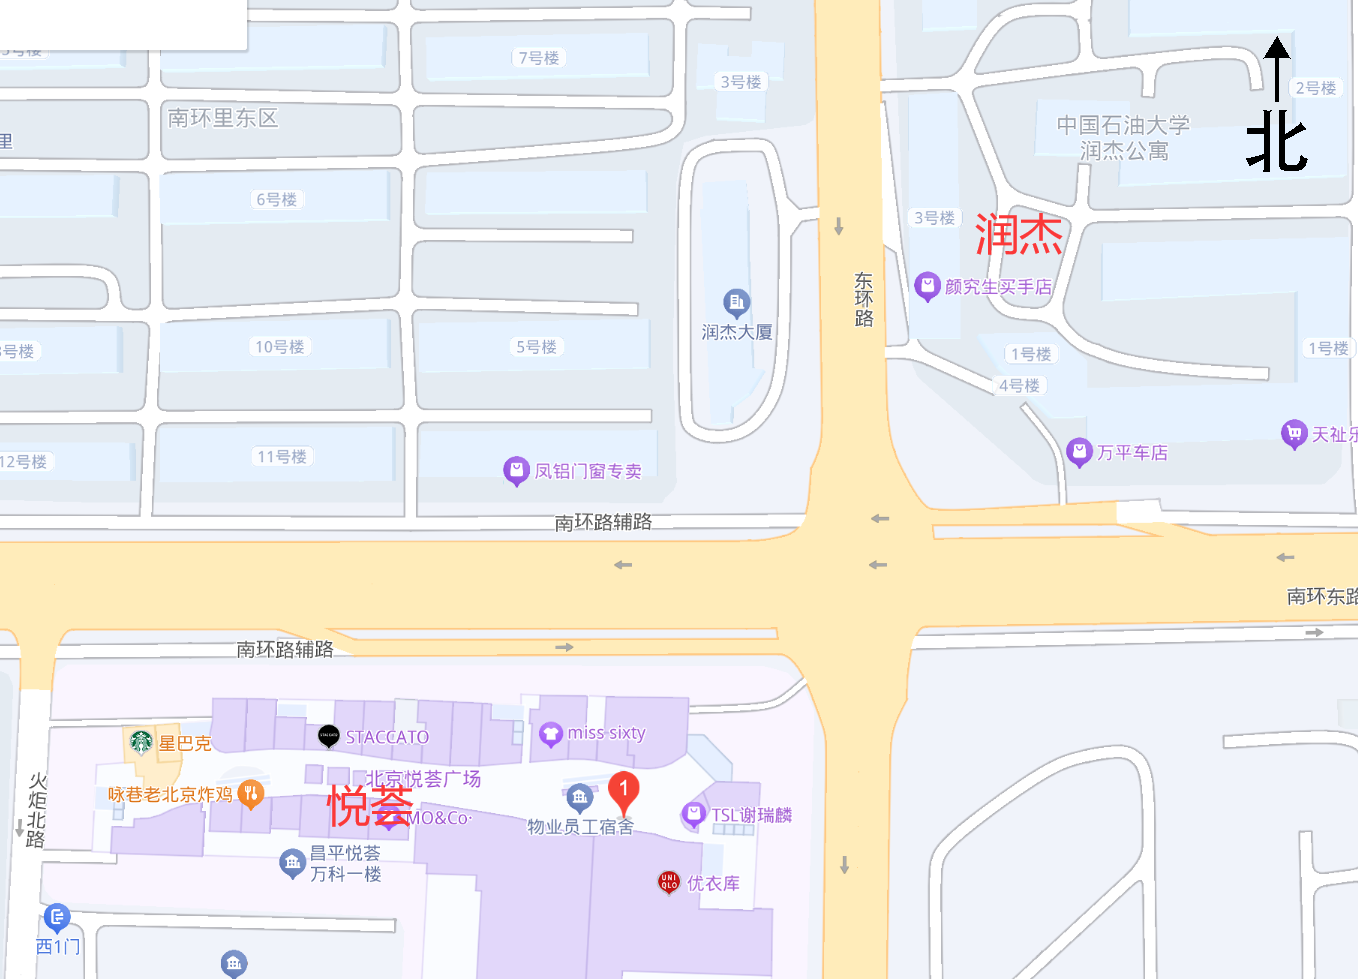
\includegraphics[width=0.6\textwidth]{pics/校外/悦荟/悦荟.png}
\end{figure}
悦荟坐落于润杰旁边,简直石大学生的第二天堂,必去的店也是多如云。大部分店都集中在五楼。

\textbf{\subsubsection*{1. 萨莉亚(提供者:Ash)}}
\addcontentsline{toc}{subsubsection}{3.6.1 \ 萨莉亚}
主要推荐:肉酱意面,烤鸡排,烤鸡腿。

我个人认为萨莉亚是在意餐的价格和品质中取了一个黄金比例的餐厅。意面和烩饭或者肉排这种主菜的话,如果你对自己的胃口比较有自信,可以多尝试一种。诚然,并不一定是每一种菜品都足够合口味,但是能用一碗兰州牛肉面的价格体验一盘肉酱意大利面,也是不错的一种选择。

顺便一提,如果你是肥宅快乐水爱好者,萨莉亚有畅饮的饮料吧,可以自行取饮。


\textbf{\subsubsection*{2. 熊喵来了(提供者:Ash)}}
\addcontentsline{toc}{subsubsection}{3.6.2 \ 熊喵来了}
熊喵来了作为在性价比市场上占据优势的火锅连锁店,近年来有与海底捞成分庭抗礼之势。

这家店的火锅底料属经典口味,肉类和涮品也属中庸。但之所以出现在这里,是因为这家店可以在美团上团购获取最优价格,并且作为招牌的一部分,鸭血和卤豆腐是免费且不限量的。

自助甜品也值得一提,甜品是免费且不限量的,你可以把吃空的甜品碟子堆起来创造奇观并且收获服务员惊愕的目光。

写在最后,据笔者个人了解,火锅底料并非清真牛油,回民同学谨慎食用。

\textbf{\subsubsection*{3. 胖哥俩肉蟹煲(提供者:Silenchatter)}}
\addcontentsline{toc}{subsubsection}{3.6.3 \ 胖哥俩肉蟹煲}
这倒没啥好说的连锁店,价格和质量都说的过去。

\textbf{\subsubsection*{4. 仙隐小鹿(提供者:Silenchatter)}}
\addcontentsline{toc}{subsubsection}{3.6.4 \ 仙隐小鹿}
日式餐厅,可以一试。有比较贵的和比较实惠的吃法,建议自行探索。

\textbf{\subsubsection*{5. 绿茶(提供者:Silenchatter)}}
\addcontentsline{toc}{subsubsection}{3.6.5 \ 绿茶}
适合3-6人聚餐。口味偏清,价格凑合,周末也是真的要排队。

\textbf{\subsubsection*{6. 文通冰室(提供者:Silenchatter)}}
\addcontentsline{toc}{subsubsection}{3.6.6 \ 文通冰室}
港式茶餐厅。这个领域内相对性价比高的一家店,多看看团购也许会有惊喜。

\textbf{\subsubsection*{7. 文立新麻辣烫(提供者:外语学院李雷锋)}}
\addcontentsline{toc}{subsubsection}{3.6.7 \ 文立新麻辣烫}
你以为东北大婶和颜悦色都是实诚人?不!精致小碟麻辣烫,宰你不留情面!

\newpage
\textbf{\subsection*{七、政法东侧一条街}}
\addcontentsline{toc}{subsection}{3.7 \ 政法东侧一条街}
\fontsize{14pt}{16.8pt}\selectfont
吃的非常之多,能在这条街上活下来的都是有点手艺的强手。

\textbf{\subsubsection*{1. 山葵村(提供者:Silenchatter)}}
\addcontentsline{toc}{subsubsection}{3.7.1 \ 山葵村}
\begin{figure}[ht]
	\centering
	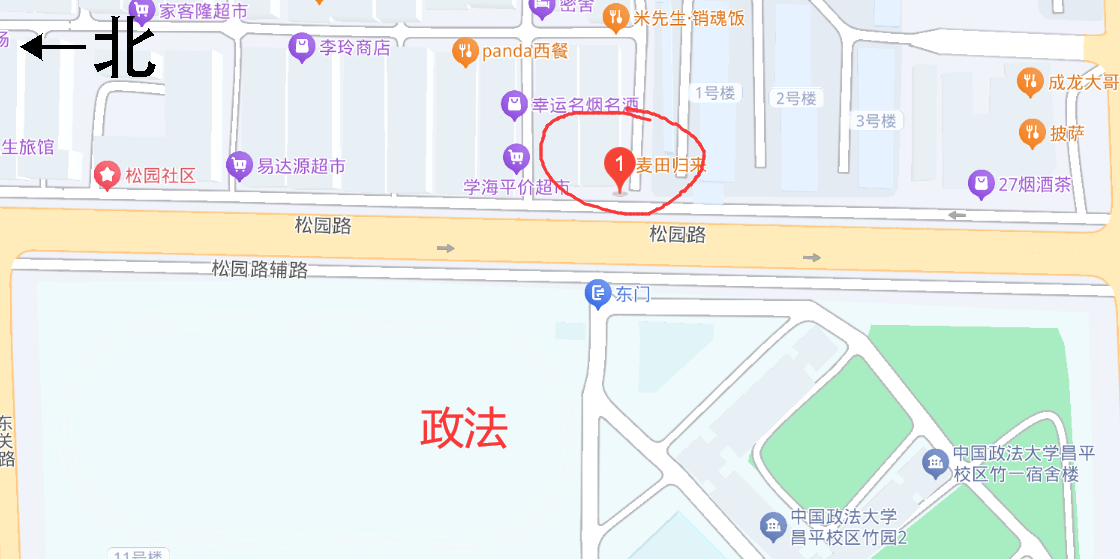
\includegraphics[width=0.73\textwidth]{pics/校外/政法/山葵村.png}
\end{figure}
新开的韩式烤肉店。经常排队,价格略高一点点。开业的时候主打一个95\%都是男店员,现在也开始招一些女店员(诚实的说他们的烤肉水平达到了普通人水准 )。

\textbf{\subsubsection*{2. 韩国肉先生(提供者:Silenchatter)}}
\addcontentsline{toc}{subsubsection}{3.7.2 \ 韩国肉先生}
\begin{figure}[ht]
	\centering
	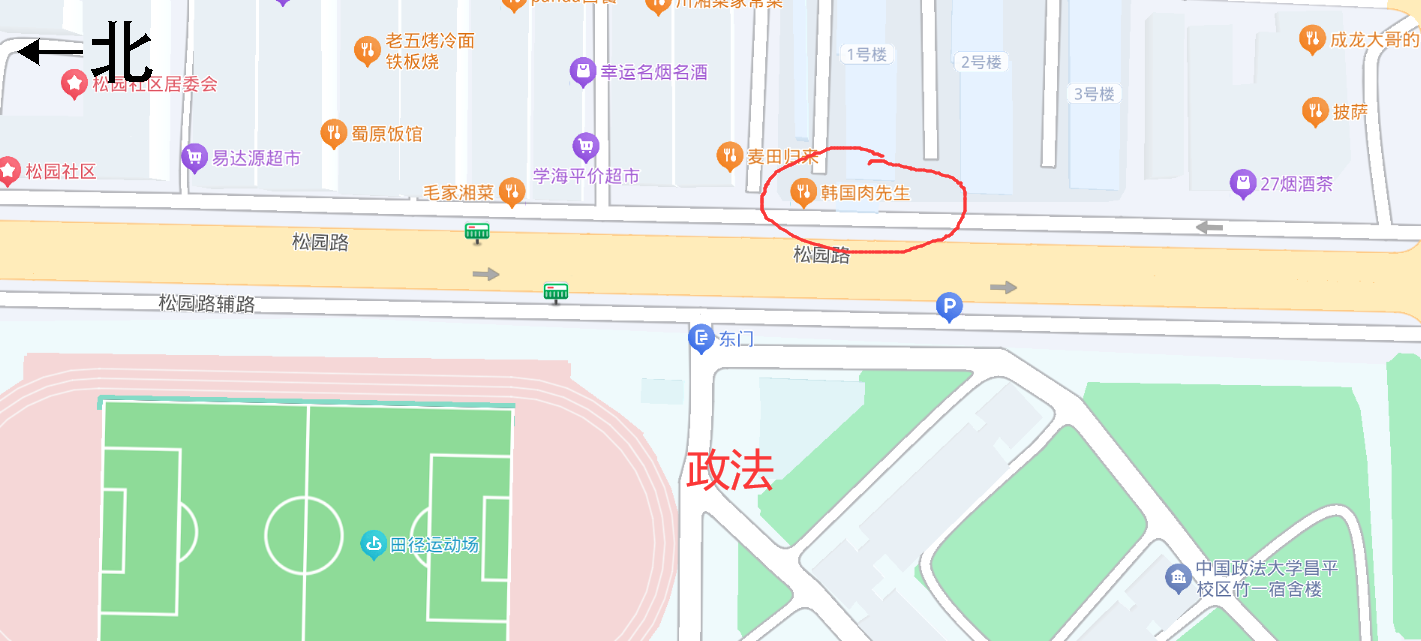
\includegraphics[width=0.73\textwidth]{pics/校外/政法/肉先生.png}
\end{figure}
是已经营业了很久的韩国烤肉店。主打一个性价比超高,环境稍微差一点。

\textbf{\subsubsection*{3. 螺老大螺蛳粉(提供者:Silenchatter)}}
\addcontentsline{toc}{subsubsection}{3.7.3 \ 螺老大螺蛳粉}
\begin{figure}[ht]
	\centering
	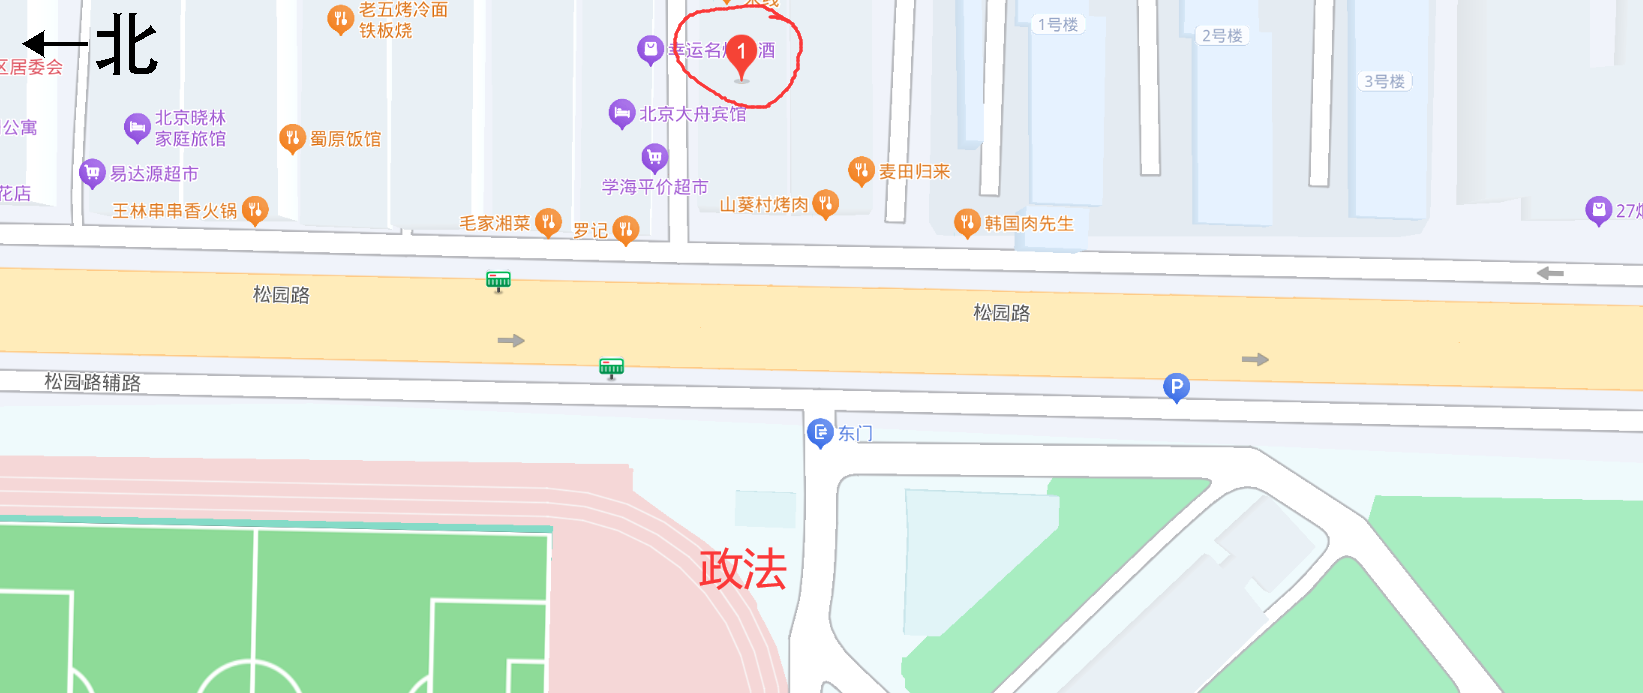
\includegraphics[width=0.73\textwidth]{pics/校外/政法/螺狮粉.png}
\end{figure}
胡同进去闻着味就找到了。之前是超超超正宗的螺蛳粉,现在也屈服了(指可以做不辣的螺蛳粉)。绿豆沙之前是买一碗可以无限量供应,现在也改成只能续一次(万恶的资本)。

\textbf{\subsubsection*{4. 蜀园(提供者:Silenchatter)}}
\addcontentsline{toc}{subsubsection}{3.7.4 \ 蜀园}
\begin{figure}[ht]
	\centering
	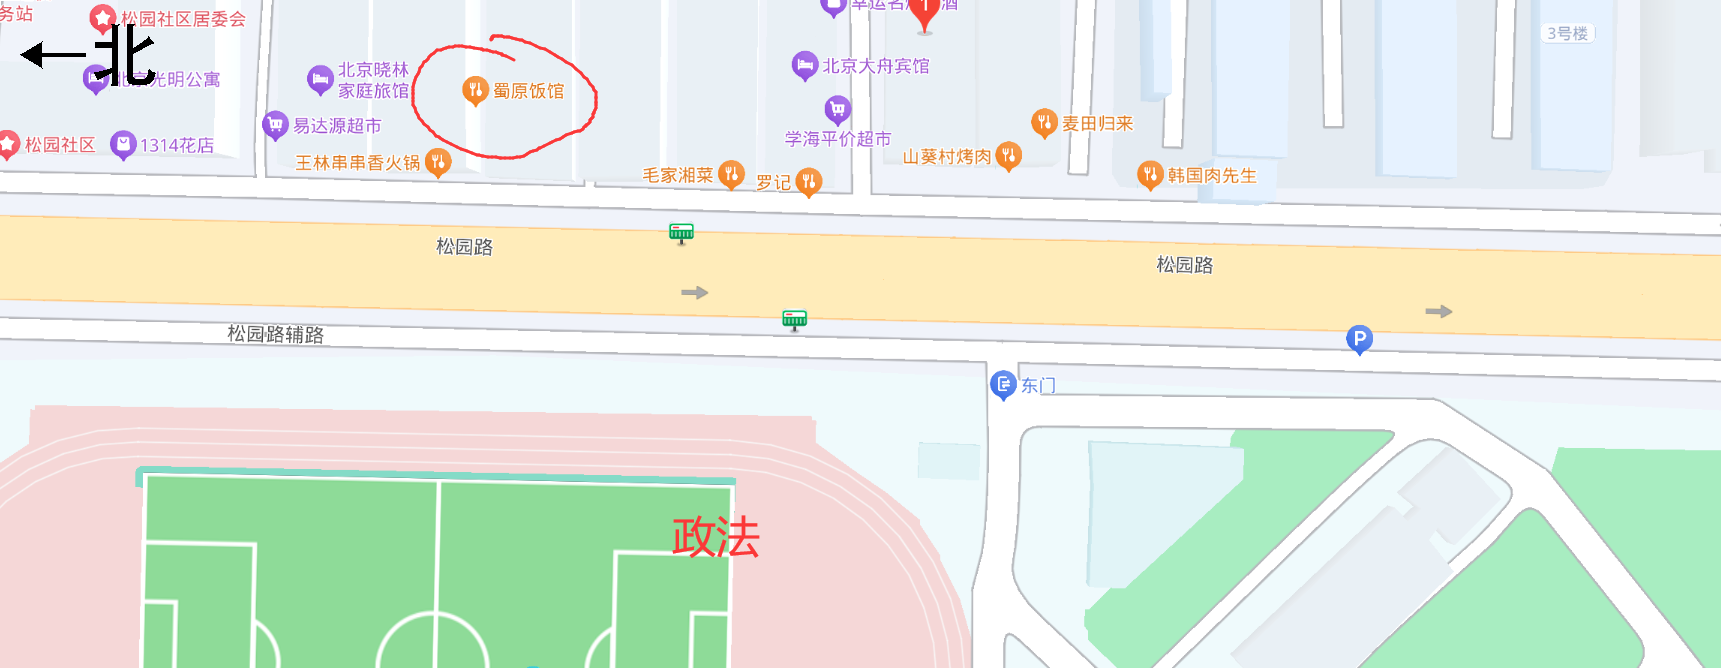
\includegraphics[width=0.73\textwidth]{pics/校外/政法/蜀园.png}
\end{figure}
川菜,多人聚餐的神(能吃一点点辣的也有能吃的菜)。价格可以接受,环境也不错。

\textbf{\subsubsection*{5. 喵lady(提供者:Silenchatter)}}
\addcontentsline{toc}{subsubsection}{3.7.5 \ 喵lady}
\begin{figure}[ht]
	\centering
	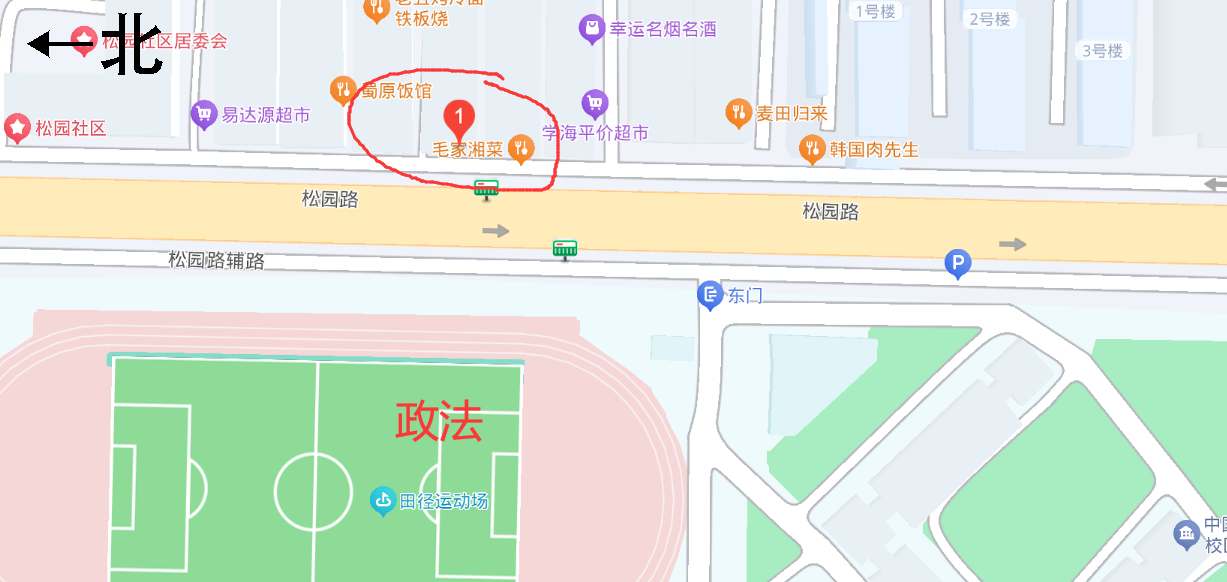
\includegraphics[width=0.73\textwidth]{pics/校外/政法/喵lady.png}
\end{figure}
猫咖,喜🐱者来。低消是一杯30左右的饮品,然后你就可以坐上一个下午(周六日人非常多,可以选一个周内的午后来玩睡觉的猫)。约会好去处。

\textbf{\subsubsection*{6. 锦州胖子烧烤/松原小刘烧烤(提供者:Silenchatter)}}
\addcontentsline{toc}{subsubsection}{3.7.6 \ 锦州胖子烧烤/松原小刘烧烤}
\begin{figure}[ht]
	\centering
	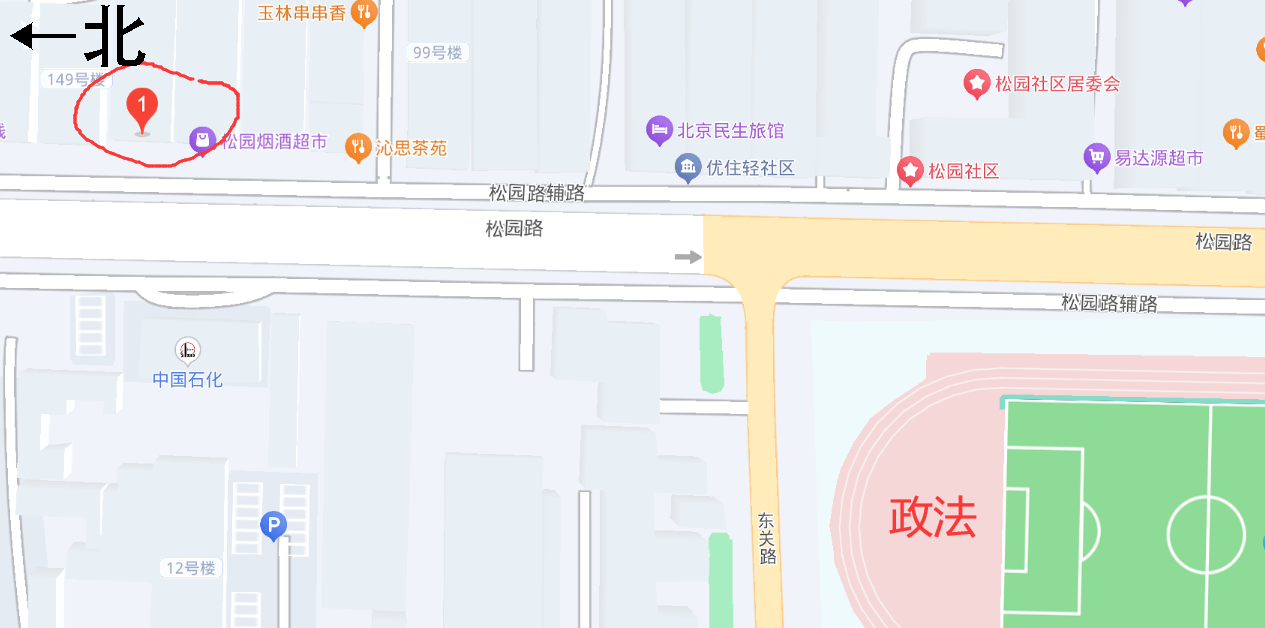
\includegraphics[width=0.73\textwidth]{pics/校外/政法/锦州.png}
\end{figure}
相对来说是能做到及格线的烧烤。在昌平城区这个地方你真的很难找到让所有人满意的烧烤,因此这里属于是可以接受的一档。

\textbf{\subsubsection*{7. 王林串串香(提供者:Silenchatter)}}
\addcontentsline{toc}{subsubsection}{3.7.7 \ 王林串串香}
性价比高,对自己肠胃的消化能力不自信的慎来。减肥的请进(不过串串嘛,哪里都是一样的拉,希望大家吃完之后有空一起拉)。
\begin{figure}[ht]
	\centering
	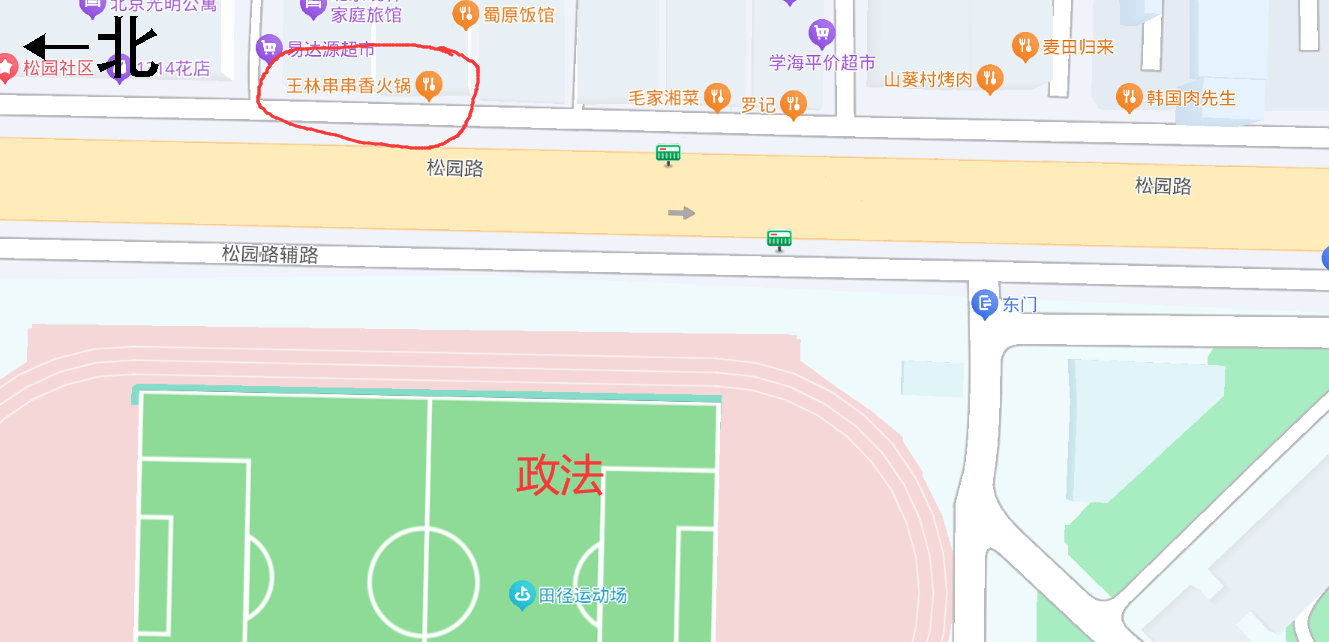
\includegraphics[width=0.73\textwidth]{pics/校外/政法/串串香.png}
\end{figure}

\newpage
\textbf{\subsection*{八、更远(待补充)}}
\addcontentsline{toc}{subsection}{3.8 \ 更远}
\fontsize{14pt}{16.8pt}\selectfont
\setlength{\parindent}{2em} % 设置首行缩进为2字符
向更远的地方拓展,包括但不限于政府街,昌平东关等。部分需要同学们提供更多资料,具体请看序言,谢谢!

\textbf{\subsubsection*{1. 晋永信刀削面(提供者:润杰梁朝伟)}}
\addcontentsline{toc}{subsubsection}{3.8.1 \ 晋永信刀削面}
\begin{figure}[ht]
	\centering
	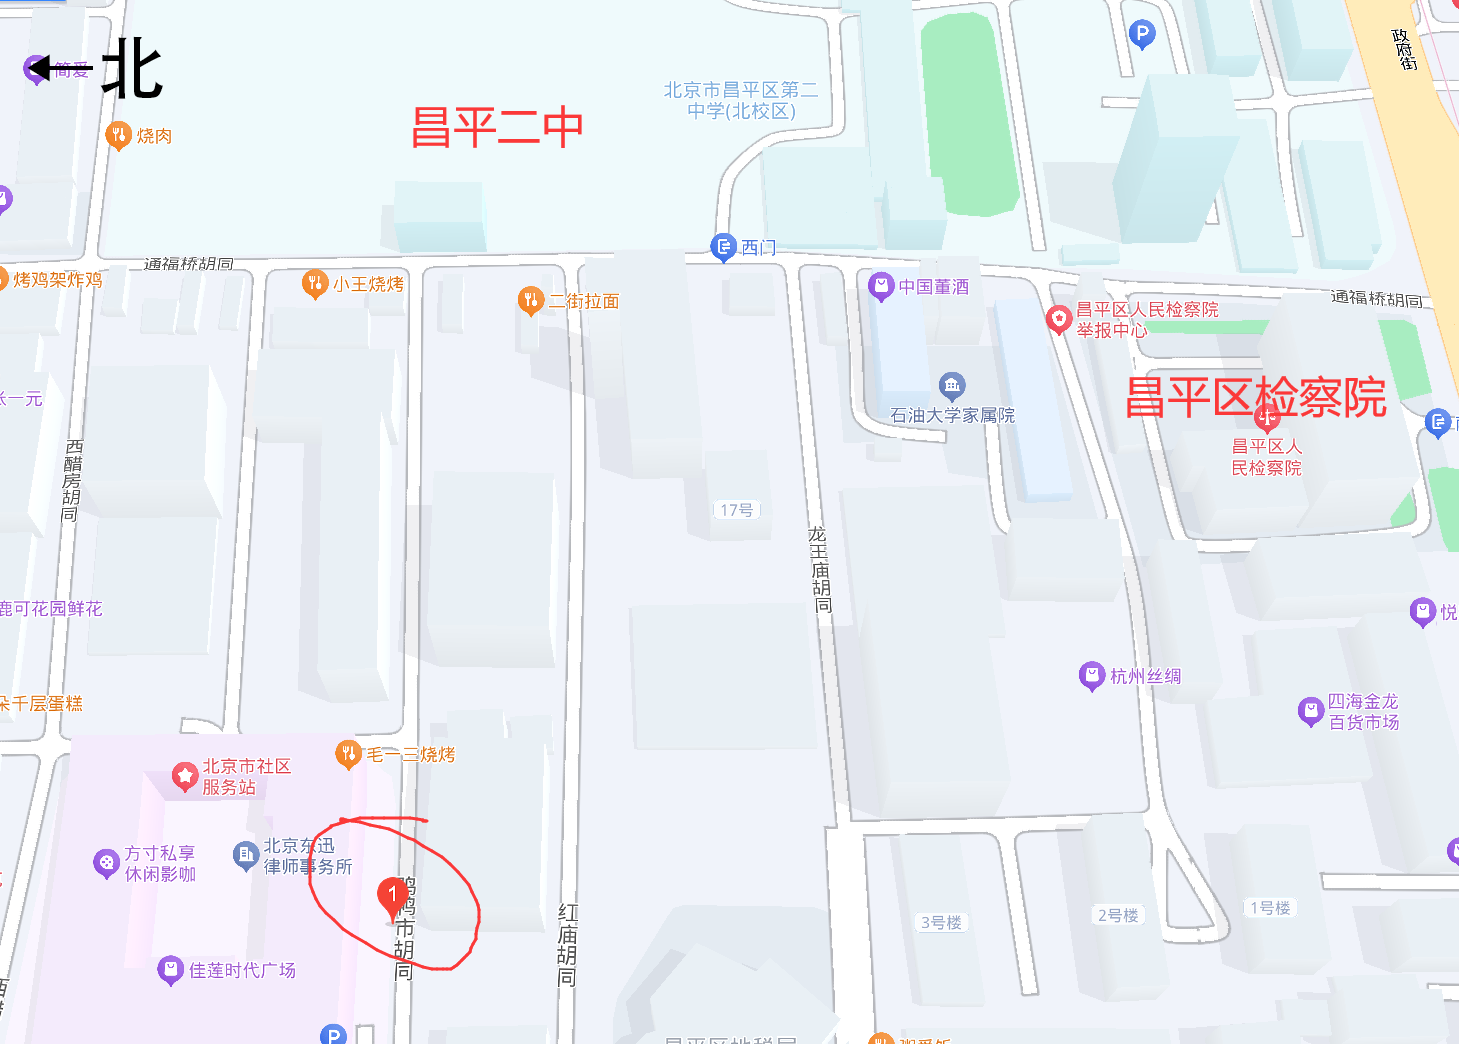
\includegraphics[width=0.73\textwidth]{pics/校外/更远/晋永信.png}
\end{figure}
个人感觉附近最好的一家刀削面,价格也在15左右,比较正常。

\textbf{\subsubsection*{2. 烤馕(提供者:润杰梁朝伟)}}
\addcontentsline{toc}{subsubsection}{3.8.2 \ 烤馕}
从晋永新刀削面吃完回宿舍发现的,这个店没有牌子,在胡同里很不显眼,从昌平二中那边来的话,一直看着胡同右边就能找到了。五块钱一个馕,谢邀,已经吃到地老天荒,好吃就完事了。
\begin{figure}[ht]
	\centering
	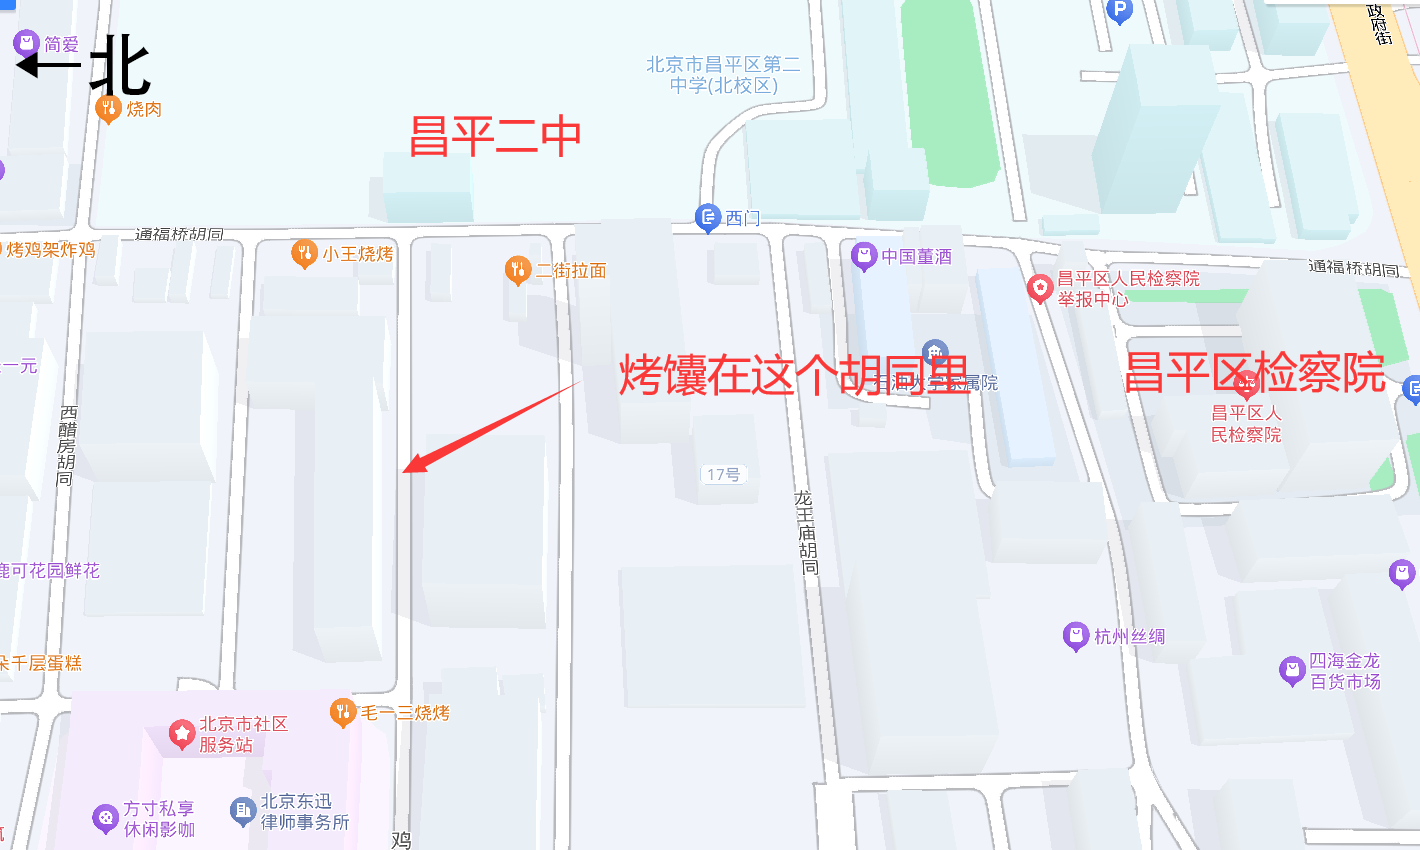
\includegraphics[width=0.73\textwidth]{pics/校外/更远/烤馕.png}
\end{figure}

\newpage
\textbf{\subsubsection*{3. 姜胖胖首尔自助烤肉(提供者:Ash)}}
\addcontentsline{toc}{subsubsection}{3.8.3 \ 姜胖胖首尔自助烤肉}
\begin{figure}[ht]
	\centering
	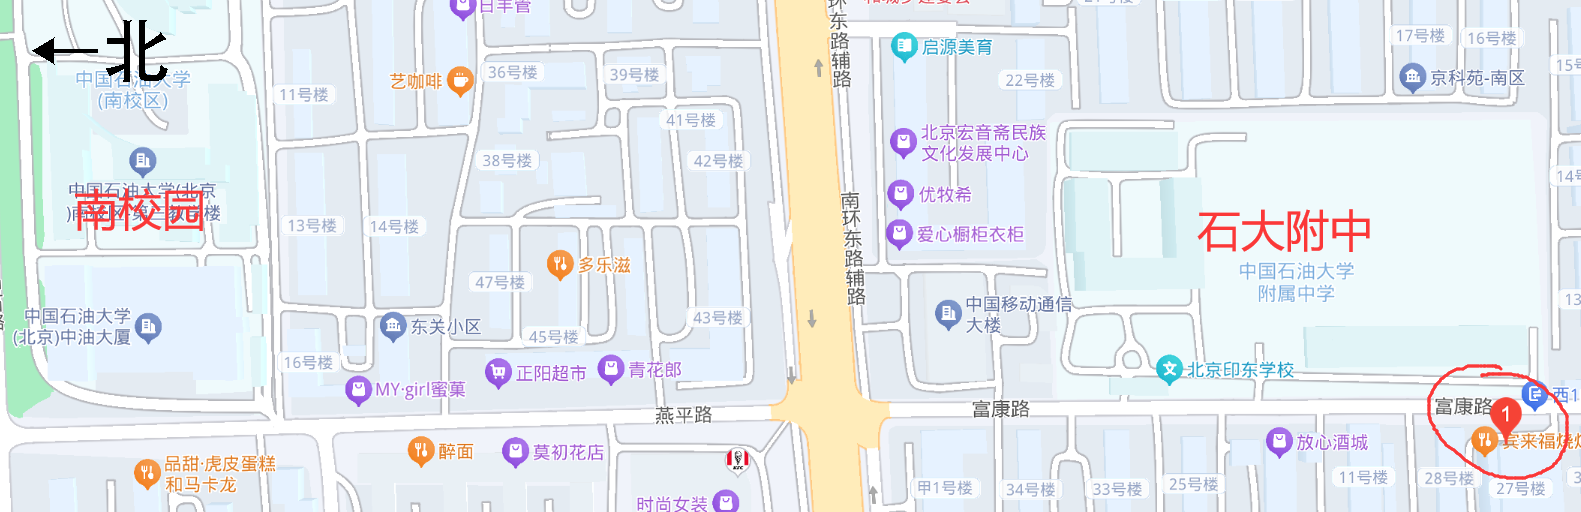
\includegraphics[width=0.73\textwidth]{pics/校外/更远/姜胖胖.png}
\end{figure}
如果你最近正在寻求烤肉的话,可以尝试一下这家自助烤肉。大约八十五块钱,名义上是韩式烤肉,但提供了各种风格的酱料因此不会囿于口味。

肉的新鲜程度尚在基准线之上,值得称道的是,这家自助烤肉会很快补满缺失的肉类,包括牛羊肉小羊排之类质量稍好的种类。同时这家店的自助冰淇淋并非掺水的合成香精,能和一部分冰淇淋店铺售卖的甜筒冰淇淋媲美,非常建议品尝。

不过除非你想当冤大头,最好不要点类似于部队锅或者韩式拉面之类的东西,有兴趣不如自己买两包韩式泡面实在。

\textbf{\subsubsection*{4. 左亭右院火锅鸡(提供者:Silenchatter)}}
\addcontentsline{toc}{subsubsection}{3.8.4 \ 左亭右院火锅鸡}
\begin{figure}[ht]
	\centering
	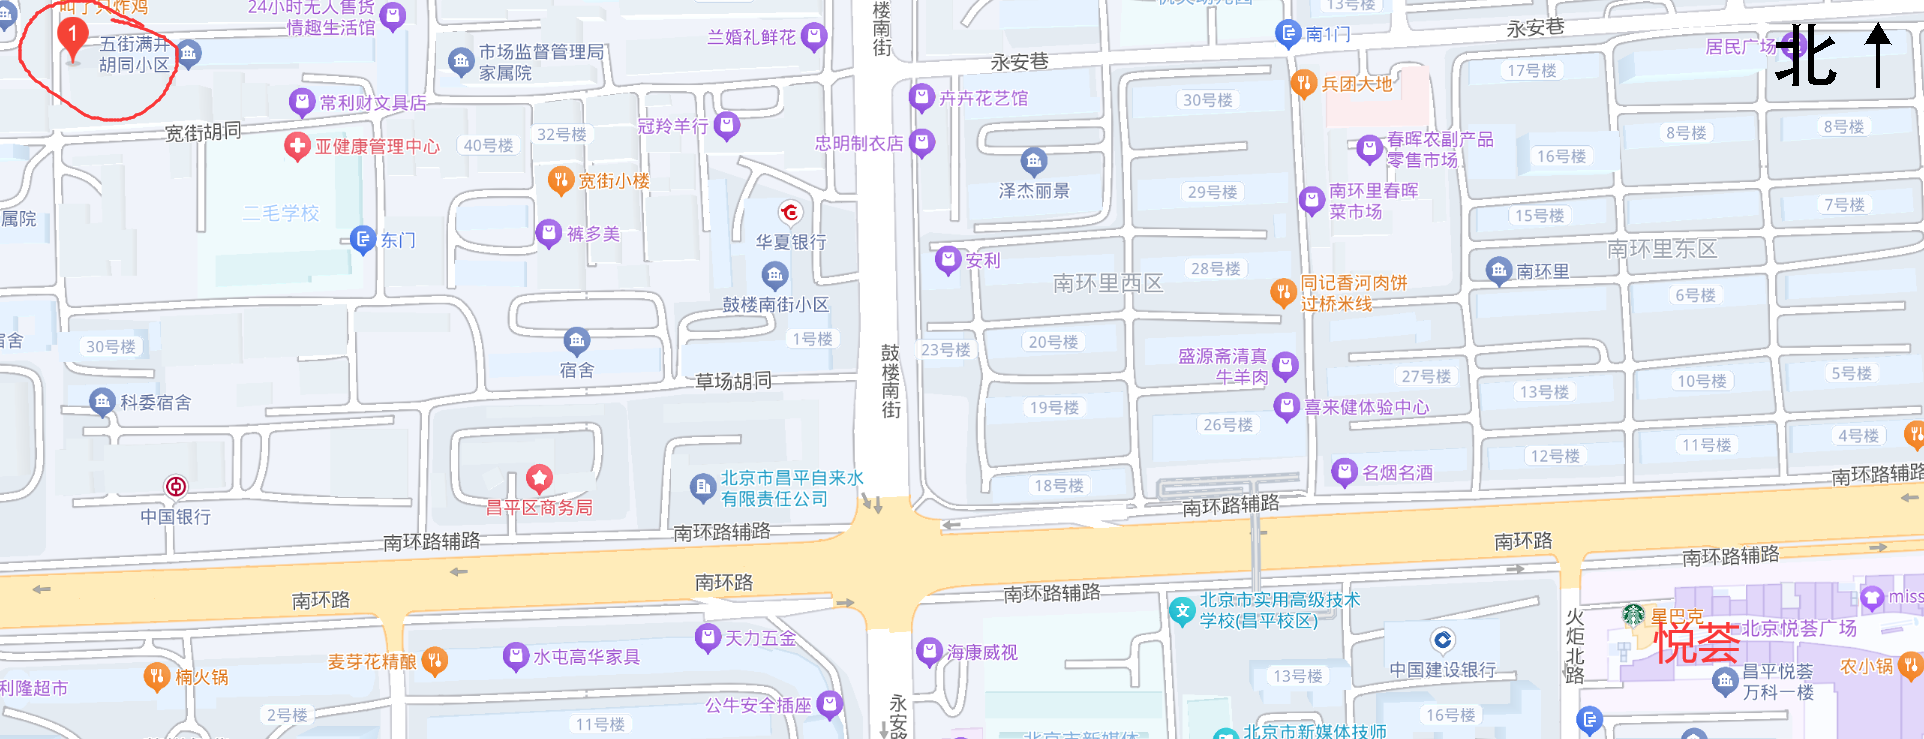
\includegraphics[width=0.73\textwidth]{pics/校外/更远/火锅鸡.png}
\end{figure}
无敌的性价比,标准的脏摊配置,以及大众认可的口味,能让这样一家藏的不能再隐蔽的店在中午十二点能等位30桌。建议早点去排队。

\textbf{\subsubsection*{5. 锦州烧烤(安福大街店)(提供者:Silenchatter)}}
\addcontentsline{toc}{subsubsection}{3.8.5 \ 锦州烧烤(安福大街店)}
\begin{figure}[ht]
	\centering
	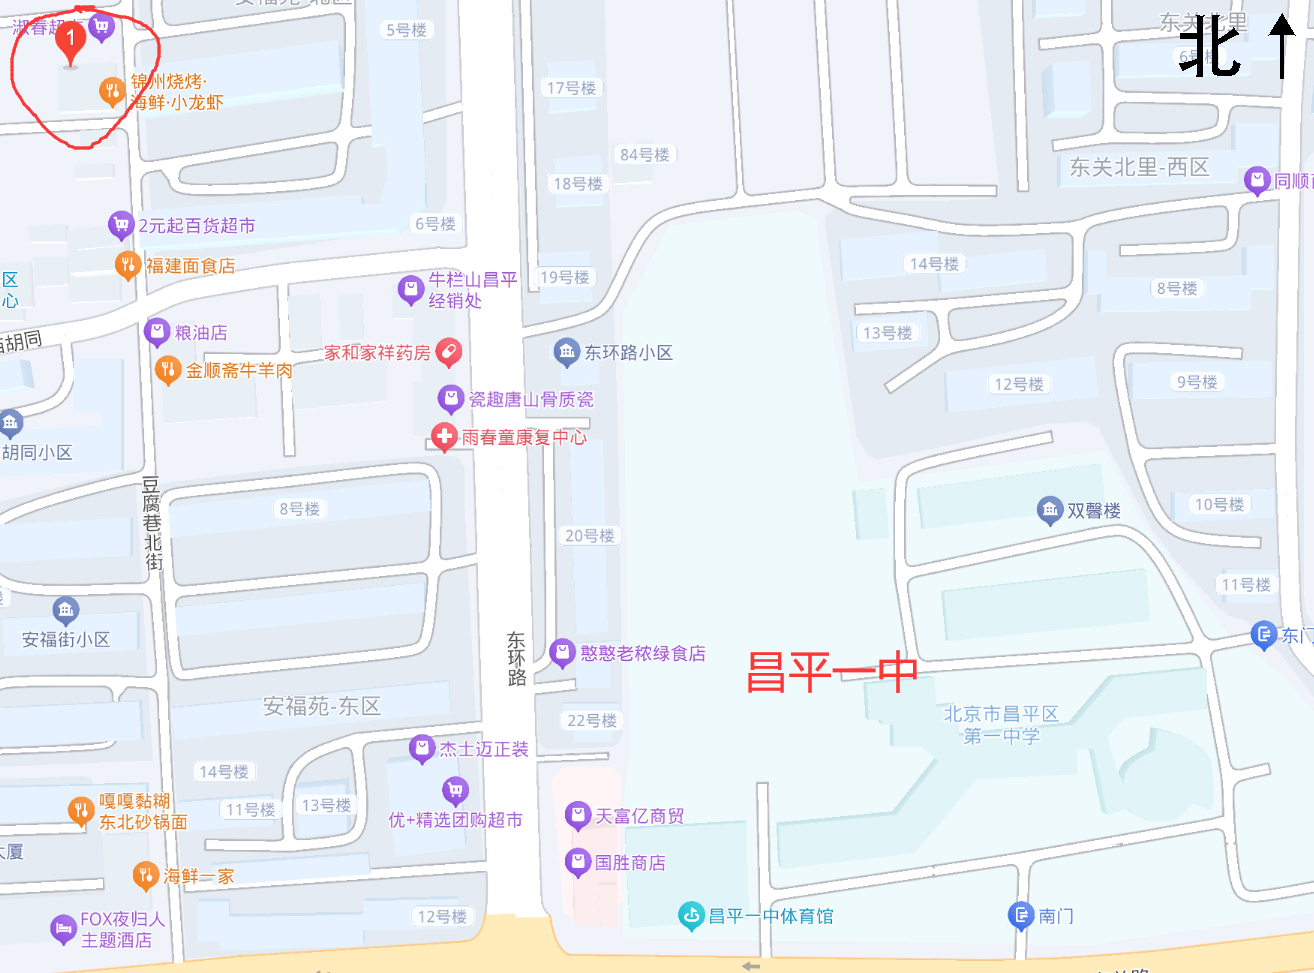
\includegraphics[width=0.73\textwidth]{pics/校外/更远/锦州.png}
\end{figure}
一些东北朋友常去的烧烤店。位置隐蔽,性价比高(本人曾有幸在店里看到一位女士单人开桌就着烧烤喝了八瓶燕京)。比标准化烧烤好吃,推荐烤豆皮。

\textbf{\subsubsection*{6. 小天地砂锅牛(提供者:Silenchatter)}}
\addcontentsline{toc}{subsubsection}{3.8.6 \ 小天地砂锅牛}
\begin{figure}[ht]
	\centering
	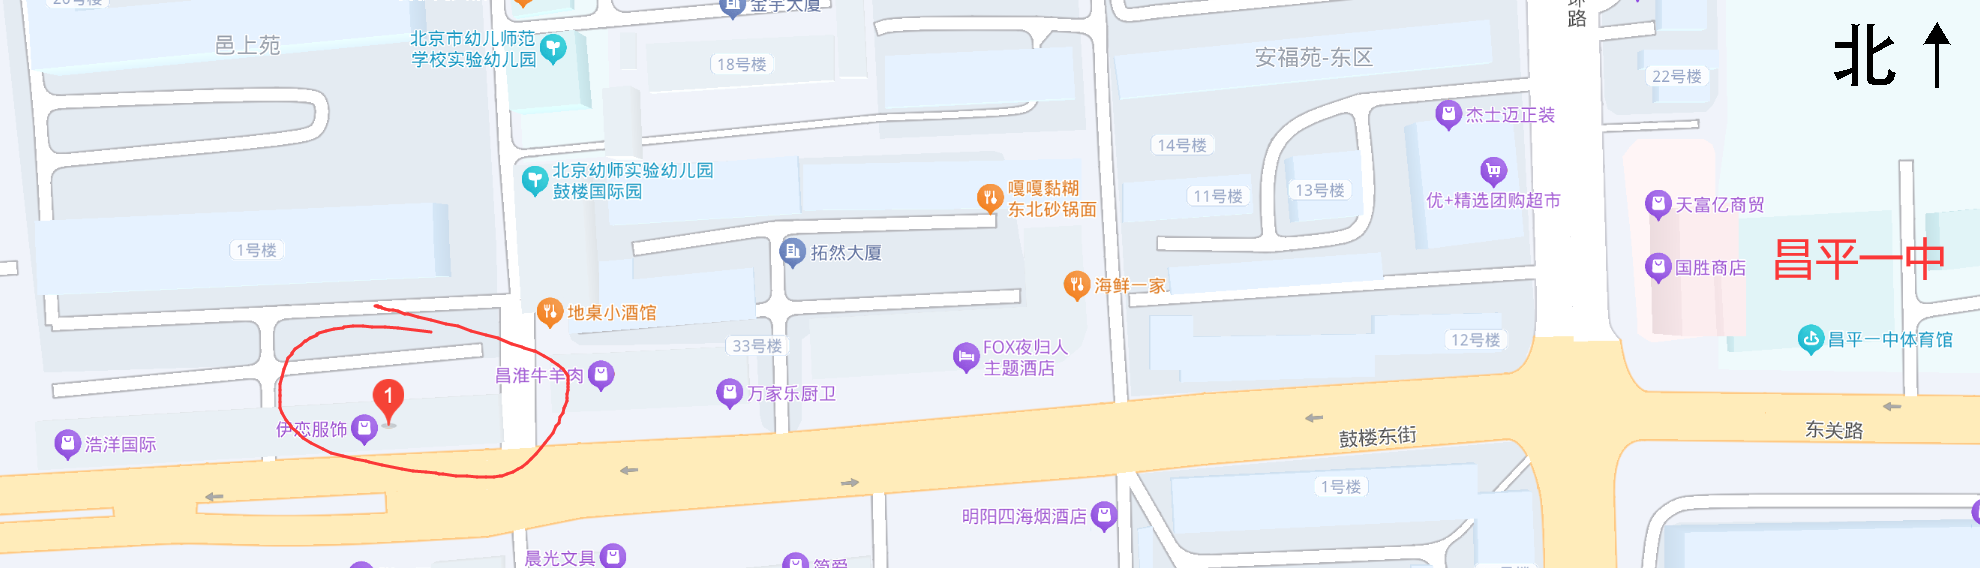
\includegraphics[width=0.73\textwidth]{pics/校外/更远/砂锅牛.png}
\end{figure}
新开没多久的店,性价比高,口味稍微清淡一些(你要是加很多辣椒也可以口味重)。强推下到锅里面的小油条。

\textbf{\subsubsection*{7. 昌顺马记小吃(提供者:Silenchatter)}}
\addcontentsline{toc}{subsubsection}{3.8.7 \ 昌顺马记小吃}
\begin{figure}[ht]
	\centering
	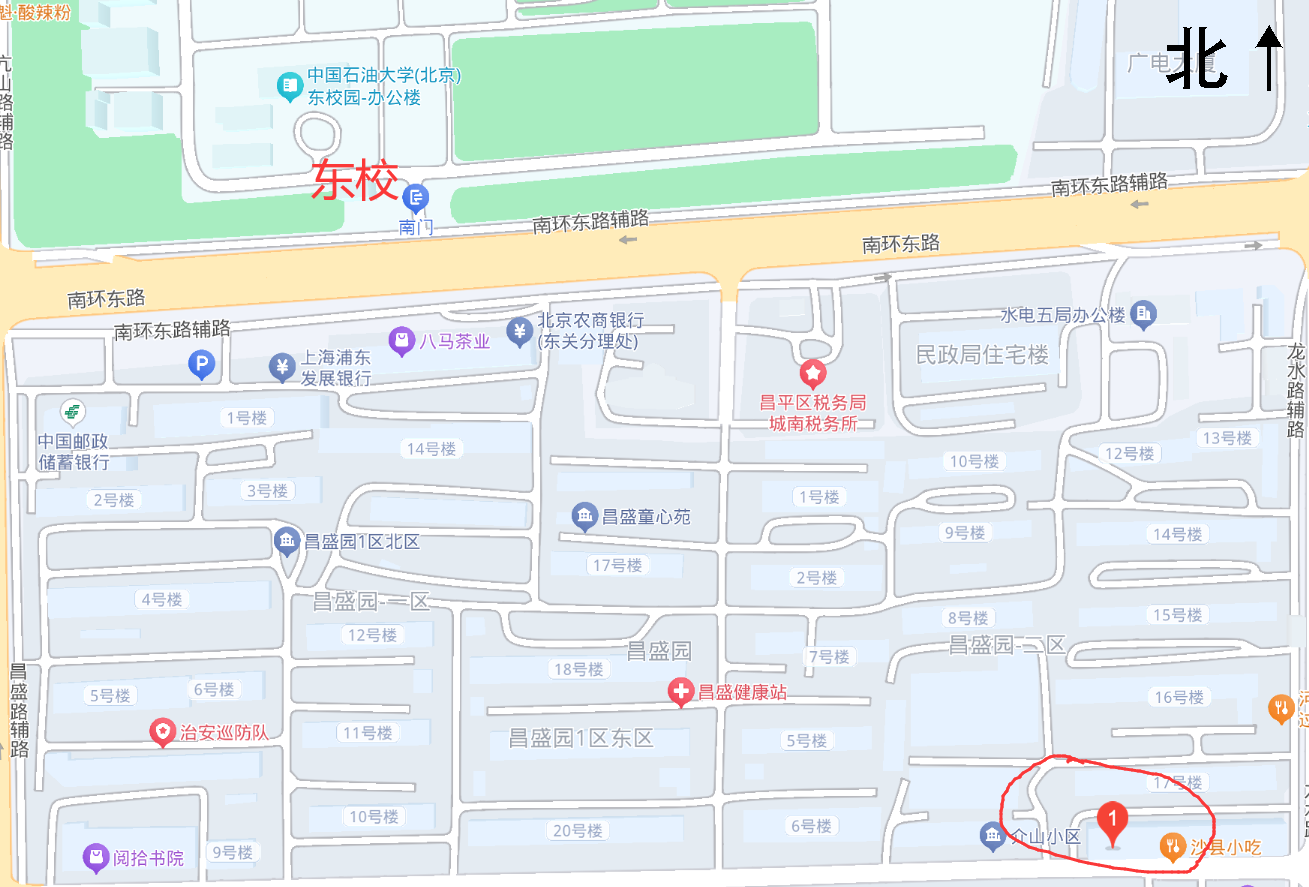
\includegraphics[width=0.73\textwidth]{pics/校外/更远/马记.png}
\end{figure}
招牌烧饼夹坛子肉,性价比超高。塞的满满当当开口超过45°的肉夹馍普通人吃两个就很饱了。他们家营业时间6-13,但是12点还是会排二三十个人左右,主打一个营业时间全程爆满。

\textbf{\subsubsection*{8. 邹三姐火锅(提供者:Silenchatter)}}
\addcontentsline{toc}{subsubsection}{3.8.8 \ 邹三姐火锅}
\begin{figure}[ht]
	\centering
	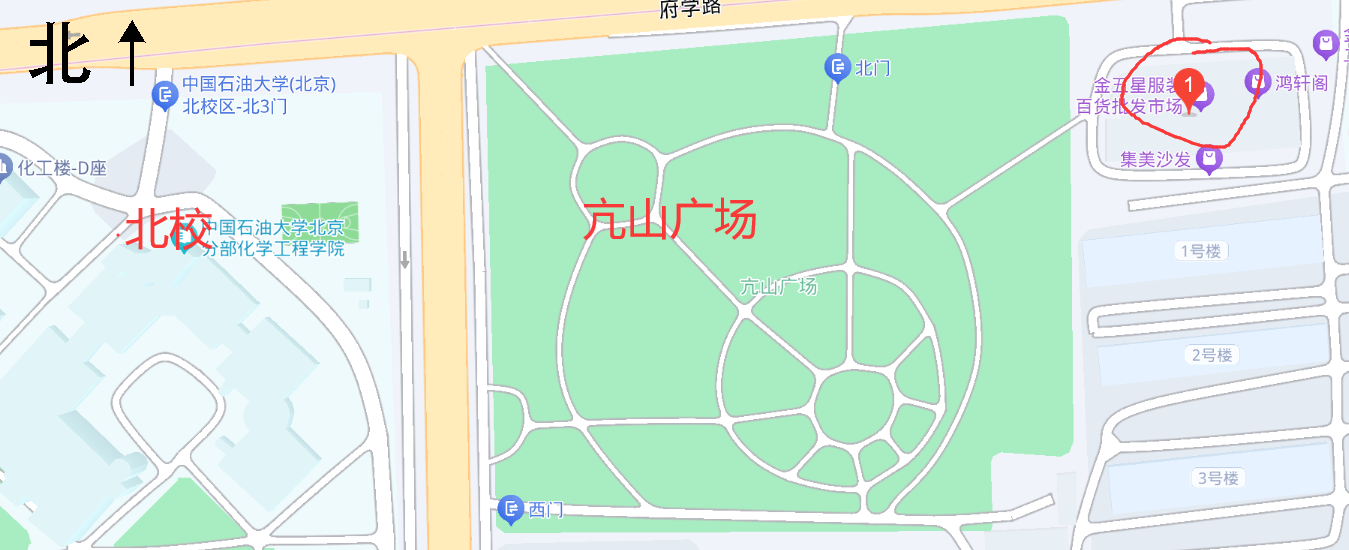
\includegraphics[width=0.73\textwidth]{pics/校外/更远/邹三姐.png}
\end{figure}
四川火锅。味道说得过去,应该算是这一片比较实惠的几家火锅之一(但是每次吃完衣服上的火锅味真的很重)。

\textbf{\subsubsection*{9. 齐齐哈尔臻兄弟烤肉(提供者:Silenchatter)}}
\addcontentsline{toc}{subsubsection}{3.8.9 \ 齐齐哈尔臻兄弟烤肉}
\begin{figure}[ht]
	\centering
	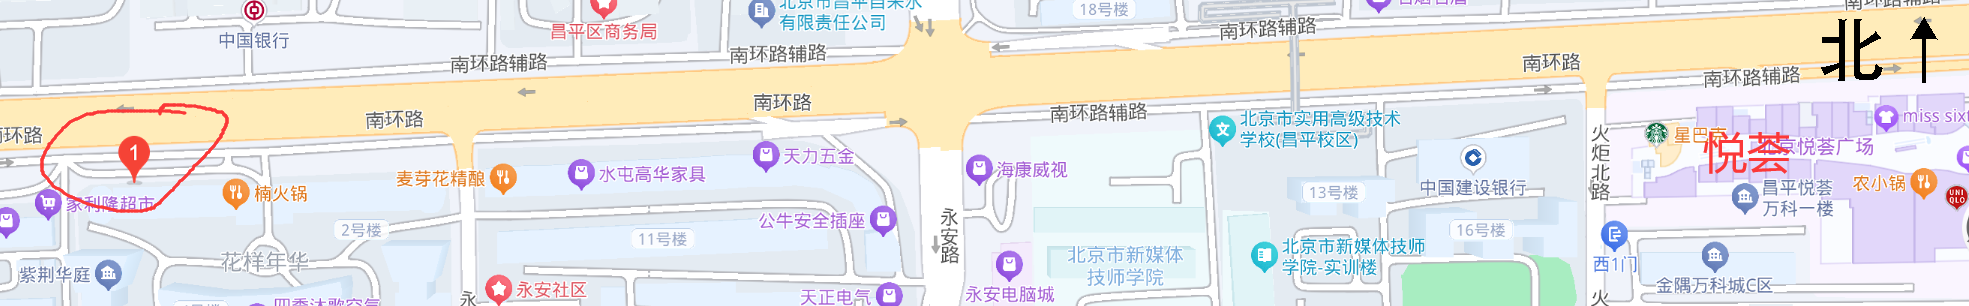
\includegraphics[width=0.77\textwidth]{pics/校外/更远/齐齐哈尔.png}
\end{figure}
蒙古烤肉。团购价格真的很好(更推荐抖音团购)。可以尝尝他们家特色的酱汁,店员会帮忙烤,味道也还不错。

\textbf{\subsubsection*{10. 山河屯铁锅炖(提供者:Silenchatter)}}
\addcontentsline{toc}{subsubsection}{3.8.10 \ 山河屯铁锅炖}
\begin{figure}[ht]
	\centering
	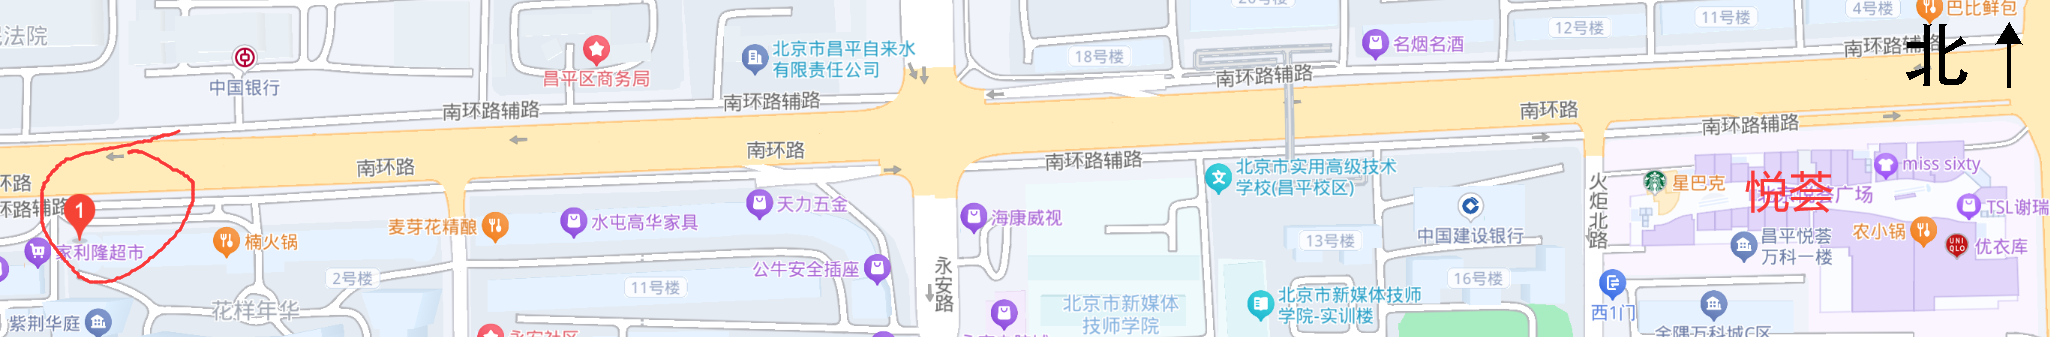
\includegraphics[width=0.77\textwidth]{pics/校外/更远/山河屯.png}
\end{figure}
身边的人有说普通的(也许是价格在铁锅炖领域里一般),但是确实稳定,是值得一试的选择。

\textbf{\subsubsection*{11. 成万富巫山烤全鱼(提供者:Silenchatter)}}
\addcontentsline{toc}{subsubsection}{3.8.11 \ 成万富巫山烤全鱼}
\begin{figure}[ht]
	\centering
	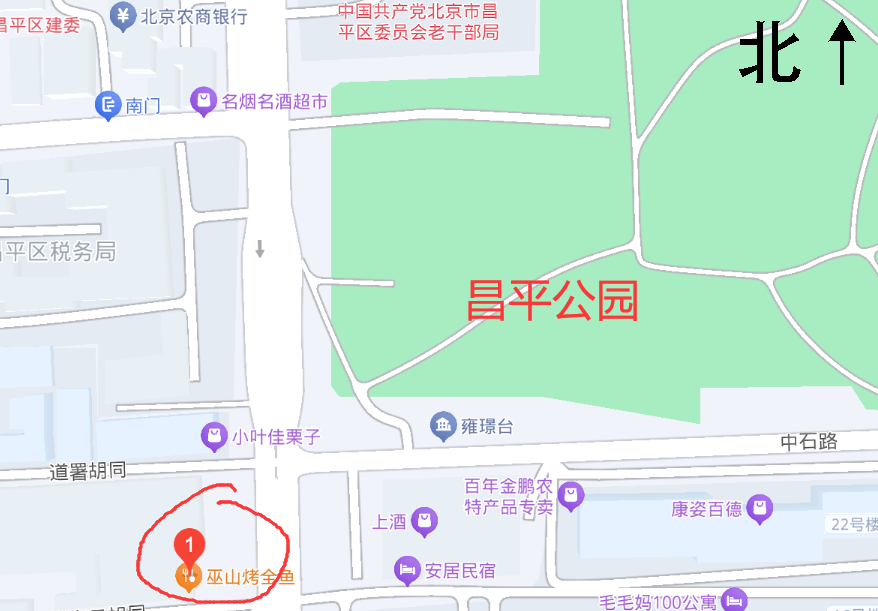
\includegraphics[width=0.65\textwidth]{pics/校外/更远/巫山.png}
\end{figure}
这是一家拥有两种流派选择的店。

如果你吃不出鱼现杀和提前杀的区别,那么就点团购(便宜)。

如果对鱼的要求比较高,那么就去店里现挑鱼杀烤来吃(略贵)。口味确实还不错(烤鸡翅也挺好)。

\textbf{\subsubsection*{12. 彭姑娘台湾车轮饼章鱼烧(提供者:Silenchatter)}}
\addcontentsline{toc}{subsubsection}{3.8.12 \ 彭姑娘台湾车轮饼章鱼烧}
\begin{figure}[ht]
	\centering
	\includegraphics[width=0.65\textwidth]{pics/校外/更远/车轮饼.png}
\end{figure}
车轮饼真的很好吃!

\newpage
\appendix
\begin{center}
	\section{鸣谢}
\end{center}

非常感谢以下同学向我提供宝贵的信息,排名按供信息时间先后顺序。

\textit{润杰梁朝伟}

\textit{橘皮}

\textit{Ash}(第二版核心作者)

\textit{Silenchatter}(第四版核心作者)

\textit{GF}

\textit{外语学院李雷锋}

\vspace{16.8pt}
感谢同学们的支持,也欢迎大家将指北宣传出去,让更多人知道;同时提供更多信息,让这份指北更加完善。没有你们就没有这份指北,谢谢!
\vspace{16.8pt}
\begin{flushright}
	\xw{刈夫}
	
	2024年9月4日

	更新于第4版
\end{flushright}

\newpage
\setlength{\parindent}{0pt} % 取消首行缩进
\begin{center}
	\section{更新日志}
\end{center}

\begin{tabularx}{\textwidth}{|>{\centering\arraybackslash}m{3cm}|X|}
    \hline
    \textbf{日期} & \multicolumn{1}{c|}{\textbf{更新内容}} \\ % 让“更新内容”居中
    \hline
    2024.8.31 & v1.0.0:完成word版初步编写 \\ 
    \hline
    2024.8.31 & v2.0.0:基本完善校内内容,新增6条3.1-3.5内容 \\ 
    \hline
    2024.9.1  & v3.0.0:\textbf{第一次重大更新} \ Latex重写排版,新增3.6悦荟 \\ 
    \hline
    2024.9.4  & v4.0.0:\textbf{第二次重大更新} \ 更换封面学校图标。删除原3.5.2胡辣汤,修正汉堡王配图错误,修正达美乐写成好利来错误,修正禾苑,KFC歧义。新增一餐内容,新增28条校外内容。修改全文字体,页面样式,附录内容。\\ 
    \hline
    2024.9.10  & v5.0.0:增加目录超链接,页面边框,更换花体页眉,更换部分字体,新增序言 \\ 
    \hline
	2024.9.17  & v5.0.1:新增3.6.7。将项目上传至github,实现开源 \\ 
    \hline
\end{tabularx}

\end{document}